\clearpage

{
    \hypersetup{linkcolor=black}
    \tableofcontents
}

\clearpage
\appendix
% \setcounter{page}{1}
% \maketitlesupplementary

\section*{Appendix}

\section{Detailed Data Sources}
\label{sec:detailed_data_sources}

Table~\ref{tab:detailed_data_sources} summarizes the task-level data source statistics of ViSTR-Bench.
For each subtask, we report the total number of video question-answer pairs and further categorize them by data source, including public datasets, curated web videos, and self-collected recordings.
We then briefly introduce the public datasets used to construct ViSTR-Bench.

\noindent\textbf{Waymo Open Dataset}~\citep{Waymo} is a large-scale autonomous driving dataset comprising 1,150 driving segments. Each segment lasts approximately 20 seconds and provides synchronized multi-view videos with rich annotations for traffic agents, including vehicles, pedestrians, and cyclists. The dataset is widely used for autonomous driving perception tasks such as 3D object detection, object tracking, and motion forecasting.
In ViSTR-Bench, we use videos from the Waymo Open Dataset~\citep{Waymo} for driving-related motion perception tasks, including Vehicle Movement and Relative Velocity. We also leverage the available vehicle annotations to localize target vehicles and overlay visual prompts on the corresponding video frames.

\noindent\textbf{ScanNet}~\citep{ScanNet} is a richly annotated RGB-D dataset of real-world indoor scenes, comprising more than 1,500 indoor scans and over 2.5 million RGB-D views. The dataset covers diverse indoor environments, such as bedrooms, offices, and living rooms. ScanNet is widely used for 3D reconstruction, semantic segmentation, and instance segmentation.
In ViSTR-Bench, we use ScanNet~\citep{ScanNet} as one of the data sources for the Ego Motion task. Given an indoor egocentric video and a target object, the model is required to infer the final spatial relationship between the observing camera and the target object.

\noindent\textbf{ScanNet++}~\citep{ScanNet++} is an extension of ScanNet~\citep{ScanNet}, offering more detailed geometry, denser visual observations, and more complete scene coverage.
It contains 460 indoor scenes, covering more than 1,000 object categories and over 21,000 object instances.
In ViSTR-Bench, we use ScanNet++~\citep{ScanNet++} as an additional data source for the Ego Motion task.

\noindent\textbf{ARKitScenes}~\citep{ARKitScenes} is a large-scale indoor RGB-D dataset captured using mobile devices equipped with LiDAR sensors. It contains 5,047 captures from 1,661 unique indoor scenes. ARKitScenes~\citep{ARKitScenes} is commonly used for 3D reconstruction, depth estimation, and indoor object detection.
In ViSTR-Bench, we use ARKitScenes~\citep{ARKitScenes} as another data source for the Ego Motion task.

\noindent\textbf{Ego4D}~\citep{Ego4D} is a large-scale egocentric video dataset that records unscripted daily human activities from a first-person perspective. It contains more than 3,700 hours of video collected by 926 participants across 74 locations in nine countries. The dataset covers diverse activities in homes, workplaces, outdoor environments, and recreational scenes. Ego4D~\citep{Ego4D} is widely used for egocentric video understanding, activity recognition, and human-object interaction analysis.
In ViSTR-Bench, we use Ego4D~\citep{Ego4D} as a public data source for outcome prediction tasks, including Basketball Shot and a subset of Billiards Shot examples.

\begin{table}[!t]
    \centering
    \caption{
        \textbf{Task-level data source statistics of ViSTR-Bench.}
        For each subtask, we report the total number of QA pairs and the number of samples collected from public datasets, curated web videos, and self-collected recordings.
    }
    \label{tab:detailed_data_sources}
    \small
    \begin{tabular}{lrrrr}
        \toprule
        \textbf{Task} & \textbf{Total} & \textbf{Public Datasets} & \textbf{Web Videos} & \textbf{Self-collected} \\
        \midrule

        \multicolumn{5}{l}{\textbf{Motion Perception}} \\
        \quad Vehicle Movement & 112 & 112 & 0 & 0 \\
        \quad Relative Velocity & 84 & 84 & 0 & 0 \\
        \midrule

        \multicolumn{5}{l}{\textbf{Spatial Relations}} \\
        \quad Ego Motion & 131 & 131 & 0 & 0 \\
        \quad Passage Feasibility & 55 & 0 & 0 & 55 \\
        \midrule

        \multicolumn{5}{l}{\textbf{Outcome Prediction}} \\
        \quad Basketball Shot & 124 & 124 & 0 & 0 \\
        \quad Soccer Shot & 158 & 0 & 158 & 0 \\
        \quad Golf Shot & 53 & 0 & 53 & 0 \\
        \quad Billiards Shot & 75 & 28 & 47 & 0 \\
        \quad Swimming Race & 72 & 0 & 72 & 0 \\
        \midrule

        \multicolumn{5}{l}{\textbf{Physical Dynamics}} \\
        \quad Jenga Stability & 117 & 0 & 0 & 117 \\
        \quad Mikado Dependency & 83 & 0 & 0 & 83 \\
        \quad Knot Type & 29 & 0 & 23 & 6 \\
        \midrule
        
        \textbf{Total} & \textbf{1093} & \textbf{479} & \textbf{353} & \textbf{261} \\
        \bottomrule
    \end{tabular}
\end{table}

\section{Detailed Prompt Templates}
\label{sec:detailed_prompt_templates}

\begin{table}[!t]
    \centering
    \caption{
        \textbf{Direct Prompting templates used in ViSTR-Bench.}
        We list the direct prompting template for each subtask.
        Placeholders such as \texttt{\{TARGET\}}, \texttt{\{OPTION\_A\}}, and \texttt{\{OPTION\_B\}} are replaced with instance-specific metadata during QA pair generation.
        % Most subtasks use fixed binary answer spaces, while Ego Motion and Swimming Race construct binary choices from relative-position labels and lane numbers, respectively.
    }
    \label{tab:direct_prompt_templates}
    \small
    \begin{tabular}{p{0.20\textwidth} p{0.70\textwidth}}
        \toprule
        \textbf{Task} & \textbf{Prompt Template} \\
        \midrule

        \multicolumn{2}{l}{\textbf{Motion Perception}} \\
        \quad Vehicle Movement
        & This is a driving video. Please determine whether the vehicle in the green box shows subtle movement during the video. Answer Yes or No. \\

        \quad Relative Velocity
        & This is a driving video. Please determine which vehicle is moving faster based on their motion over time: the vehicle in the green box or the vehicle in the blue box. Answer Green or Blue. \\
        \midrule

        \multicolumn{2}{l}{\textbf{Spatial Relations}} \\
        \quad Ego Motion
        & This is a video recorded by a moving camera in an indoor scene. The target object is the \texttt{\{TARGET\}}. Please determine the final position of the target object relative to the camera. Is it \texttt{\{OPTION\_A\}} or \texttt{\{OPTION\_B\}}? Answer \texttt{\{OPTION\_A\}} or \texttt{\{OPTION\_B\}}. \\

        \quad Passage Feasibility
        & This is a video of a vehicle and traffic cones placed near its driving path. Please predict whether the vehicle can pass the cone-constrained area without touching any cone. Answer Yes or No. \\
        \midrule

        \multicolumn{2}{l}{\textbf{Outcome Prediction}} \\
        \quad Basketball Shot
        & This is a video of a basketball shot. Please predict whether the basketball will go into the hoop. Answer Yes or No. \\

        \quad Soccer Shot
        & This is a video of a soccer free kick. Please predict whether the ball will go into the goal based on its trajectory, ignoring the goalkeeper and any defensive interference. Answer Yes or No. \\

        \quad Golf Shot
        & This is a video of a golf shot. Please predict whether the golf ball will go into the hole based on its observed trajectory. Answer Yes or No. \\

        \quad Billiards Shot
        & This is a video of billiards. Please predict whether the target ball will go into the pocket based on its current trajectory. Answer Yes or No. \\

        \quad Swimming Race
        & This is a video of a swimming race. The swimmer at the top of the frame is in lane 1, and the lane numbers increase from top to bottom. Please determine which swimmer will reach the finish line first between lane \texttt{\{OPTION\_A\}} and lane \texttt{\{OPTION\_B\}}. Answer \texttt{\{OPTION\_A\}} or \texttt{\{OPTION\_B\}}. \\
        \midrule

        \multicolumn{2}{l}{\textbf{Physical Dynamics}} \\
        \quad Jenga Stability
        & This is a video of a Jenga game. Please predict whether the tower will remain stable after the block that the hand is trying to pull out is removed. Answer Yes or No. \\

        \quad Mikado Dependency
        & This is a video of a Mikado game. Please predict whether the stick indicated by the pointing stick can be picked up without touching any other sticks. Answer Yes or No. \\

        \quad Knot Type
        & This is a video of knot manipulation. Please determine whether the knot is a slip knot (can be undone by pulling one end) or a fixed knot (cannot be undone and remains tight when pulled). Answer Slip or Fixed. \\
        \bottomrule
    \end{tabular}
\end{table}

\subsection{Direct Prompting}

Table~\ref{tab:direct_prompt_templates} presents the Direct Prompting templates used in ViSTR-Bench.
Each prompt specifies the visual context, the reasoning target, and the required answer format for the corresponding subtask.
Placeholders such as \texttt{\{TARGET\}}, \texttt{\{OPTION\_A\}}, and \texttt{\{OPTION\_B\}} are replaced with instance-specific metadata during QA pair generation.
Most subtasks adopt fixed binary answer spaces, including Yes/No for judgment tasks, Green/Blue for comparing prompted vehicles, and Slip/Fixed for knot classification.
For the remaining subtasks, Ego Motion constructs binary choices from relative-position labels, including front-left, front-right, back-left, and back-right, whereas Swimming Race constructs binary choices from lane numbers.

\subsection{Manual CoT}

Inspired by OmniSpatial~\citep{OmniSpatial}, Manual CoT explicitly decomposes each task into visually grounded intermediate reasoning steps.
This design differs from existing methods such as Zero-shot CoT~\citep{zero-shot-cot}, Self-Consistency~\citep{self-consistency-coT}, and Plan-and-Solve~\citep{plan-and-solve}, which rely on generic reasoning instructions or repeated sampling with the same prompt.
Specifically, we manually design a task-specific reasoning procedure for each subtask in ViSTR-Bench, guiding the model to first identify the relevant visual target, then track task-specific spatial-temporal evidence across the video, and finally produce the prediction using the prescribed answer format.
The complete Manual CoT prompt templates are shown in Figures~\ref{fig:6}-\ref{fig:17}.

\section{Model and Inference Details}
\label{sec:model_inference_details}

For general-purpose MLLMs, we adopt different input formats depending on whether each model natively supports video input.
For Gemini-3/3.1~\citep{Gemini}, Seed-2.0~\citep{Seed}, MiMo-V2/V2.5~\citep{MiMo-V2-Omni,MiMo-V2.5}, Qwen3.5~\citep{Qwen3.5}, and GLM-4.6V~\citep{GLM-4.6V}, we directly provide the original video clip as the visual input.
The maximum video resolution is constrained to $1920 \times 1280$, and the maximum Base64-encoded video size is set to 10 MB.
For GPT-5.4~\citep{GPT-5}, Claude-4.6~\citep{Claude}, Intern-S1~\citep{Intern-S1,Intern-S1-Pro}, and InternVL3.5~\citep{InternVL3.5}, we convert each video into a sequence of sampled frames.
Specifically, we uniformly sample 16 frames from each video and constrain the maximum image resolution to $1280 \times 720$.
The sampled frames are provided together with a short textual instruction indicating that they are sampled from the same video and arranged in chronological order, followed by the task question.
For model-specific inference settings, we set the thinking level of GPT-5.4~\citep{GPT-5} to \texttt{xhigh}.
For Gemini-3/3.1~\citep{Gemini}, we set the temperature to 1.0, top-$p$ to 0.95, top-$k$ to 64, the maximum output length to 65,536 tokens, and the thinking level to \texttt{high}.
For Claude-4.6~\citep{Claude}, we set the maximum output length to 16,000 tokens and the thinking budget to 1,024 tokens.
Finally, for specialized spatial MLLMs, we run their official source code with the default inference settings.

\section{Error Analysis}
\label{sec:error_analysis}

To better investigate why current MLLMs exhibit limited performance on ViSTR-Bench, we conduct an error analysis of the 481 incorrect predictions made by Gemini-3.1-Pro-Preview~\citep{Gemini} under the Manual CoT setting.
For each incorrect prediction, we assign one primary error type based on the task definition, the ground-truth answer, and the reasoning steps generated by the model following the Manual CoT prompt.

\subsection{Error Categorization}

We define six task-agnostic primary error types to characterize the major failure modes observed across different subtasks.
Representative examples for each error category are illustrated in Figure~\ref{fig:18}.

\noindent\textbf{Target Identification Error.} % Billiards Shot
The model fails to reliably identify the target object specified in the question.
Typical examples include confusing the target ball in Billiards, mixing up lane numbers in Swimming Race, and localizing the wrong Jenga block or Mikado stick.

\noindent\textbf{Target Tracking Error.} % Basketball Shot, Soccer Shot, Golf Shot, Billiards Shot
The model correctly identifies the target but fails to continuously track its trajectory over time.
Typical examples include losing track of a moving ball or confusing its position across consecutive frames.

\noindent\textbf{Motion State Error.} % Vehicle Movement, Relative Velocity
The model correctly identifies the prompted vehicles but misjudges their motion state.
Typical cases include missing subtle vehicle movement in Vehicle Movement or incorrectly identifying the faster vehicle in Relative Velocity.

\noindent\textbf{Outcome Reasoning Error.} % Basketball Shot, Soccer Shot, Golf Shot, Billiards Shot, Swimming Race
The model correctly observes the current motion or state but fails to infer the correct final outcome.
Typical cases include incorrectly predicting whether a shot will succeed or which swimmer will reach the finish line first.

\noindent\textbf{Spatial Relation Error.} % Ego Motion, Passage Feasibility
The model incorrectly estimates spatial relations between the target and reference objects.
Representative cases include reversing observer-centric directions in Ego Motion or misjudging whether a vehicle has sufficient spatial clearance to pass through a cone-constrained region in Passage Feasibility.

\noindent\textbf{Physical Interaction Error.} % Jenga Stability, Mikado Dependency, Knot Type
The model incorrectly reasons about latent physical properties, dependencies, or stability conditions.
For example, the model may misjudge whether a Mikado stick is blocked by another stick, whether a Jenga block is load-bearing, or whether a specific knot can be released by pulling one end.

\begin{table}[!t]
    \centering
    \caption{
        \textbf{Distribution of primary error types.}
        We analyze the 481 incorrect predictions made by Gemini-3.1-Pro-Preview~\citep{Gemini} under the Manual CoT setting.
        Each incorrect prediction is assigned one primary error type.
    }
    \label{tab:error_distribution}
    \small
    \begin{tabular}{lrr}
        \toprule
        \textbf{Primary Error Type} & \textbf{\#Errors} & \textbf{Ratio} \\
        \midrule
        Outcome Reasoning Error & 156 & 32.4\% \\
        Physical Interaction Error & 101 & 21.0\% \\
        Motion State Error & 95 & 19.7\% \\
        Spatial Relation Error & 61 & 12.7\%  \\
        Target Tracking Error & 59 & 12.3\% \\
        Target Identification Error & 9 & 1.9\%  \\
        \midrule
        \textbf{Total} & \textbf{481} & \textbf{100.0\%} \\
        \bottomrule
    \end{tabular}
\end{table}

\subsection{Error Statistics}

Table~\ref{tab:error_distribution} reports the distribution of the primary error types.
\emph{Outcome Reasoning Error} is the most frequent category. These cases indicate that even when the model captures the current motion or intermediate state, it often fails to extrapolate these cues to the correct final outcome.
\emph{Physical Interaction Error} is mainly observed in Jenga Stability, Mikado Dependency, and Knot Type, showing that current MLLMs have limited ability to infer latent physical properties, object dependencies, and stability conditions.
\emph{Motion State Error} is the third-largest category, suggesting that current MLLMs still struggle to determine whether a prompted object is moving and to compare motion-related attributes such as relative speed.
\emph{Spatial Relation Error} mainly arises in Ego Motion and Passage Feasibility, where the model either reverses observer-centric directions or misjudges the spatial clearance between a vehicle and surrounding obstacles.
\emph{Target Tracking Error} reflects failures in continuously following the target trajectory over time, especially in ball-centric outcome prediction tasks.
\emph{Target Identification Error} accounts for only 9 cases, mostly occurring in Billiards, where the model confuses the target ball with other balls on the table.
Overall, the error distribution shows that the main bottlenecks of current MLLMs on ViSTR-Bench are not simple failures to recognize target objects.
Instead, the dominant limitations lie in predicting motion states and attributes, tracking dynamic visual evidence over time, extrapolating observed states to future outcomes, and reasoning about latent physical interactions.

\section{Preliminary Exploration on Model Improvement}
\label{sec:model_improvement}

The error analysis shows that current MLLMs still struggle to reason from continuous visual cues in dynamic scenes.
Based on these observations, we discuss several complementary directions for improving model performance.
First, a data-centric direction is to construct larger-scale training data specifically designed for dynamic spatial-temporal reasoning.
Although current MLLMs are trained on massive image-text and video-text corpora, existing datasets~\citep{SPAR-Bench,LLaVA-Video} mainly focus on static visual recognition or general video understanding, and provide limited supervision for fine-grained dynamic reasoning.
Second, an input-centric direction is to enrich the visual input with more explicit spatial evidence beyond the original camera trajectory.
For example, auxiliary novel views can be rendered from the reconstructed scene and added to the original video, providing complementary geometric and layout cues that are not directly observed from the captured viewpoints.
Third, a tool-augmented direction is to build agentic systems that decompose complex video reasoning problems into intermediate subproblems and use external tools to extract task-relevant visual evidence.
For instance, detectors and trackers can localize target objects, optical flow can estimate motion patterns, and 3D reconstruction can recover scene geometry.
This paradigm is promising because it offloads low-level visual perception to specialized tools, allowing MLLMs to focus more on high-level spatial-temporal reasoning.

As a preliminary exploration, we investigate the input-centric direction on the Ego Motion task.
We select GPT-5.4-thinking~\citep{GPT-5}, the best-performing model on this task, and augment the 16-frame baseline with 10 rendered auxiliary views.
Specifically, we first reconstruct the 3D scene from the original video using VGGT-$\Omega$~\citep{VGGT-Omega}, and then render novel views as additional spatial evidence for the model.
This simple augmentation improves the accuracy from 75.6\% to 80.2\%, indicating that auxiliary rendered views can make useful spatial cues more accessible to current MLLMs.
Rather than proposing a complete solution, this preliminary study aims to examine whether geometry-enhanced inputs can benefit dynamic scene reasoning, thereby highlighting a promising direction for improving the spatial-temporal reasoning ability of current MLLMs.

\section{Qualitative Visualizations}
\label{sec:visualization}

We provide qualitative visualizations for all 12 tasks in ViSTR-Bench.
For each task, we select one representative example and visualize the model outputs from GPT-5.4-thinking~\citep{GPT-5}, Gemini-3.1-Pro-Preview~\citep{Gemini}, and Claude-Opus-4.6-thinking~\citep{Claude}.
The results are shown in Figures~\ref{fig:19}-\ref{fig:30}.

\section{Limitations and Future Work}
\label{sec:limitations_future_work}

While ViSTR-Bench provides a diagnostic testbed for visual spatial-temporal reasoning, it also has several limitations that motivate future research.

\noindent\textbf{Task and data coverage.}
ViSTR-Bench covers 12 subtasks across tabletop, indoor, and outdoor scenarios, but it is not intended to exhaust all forms of spatial-temporal reasoning in the physical world.
The current benchmark focuses on relatively short clips with clearly specified targets and binary decisions.
In contrast, many real-world embodied tasks require longer-horizon planning, multi-agent interaction, and adaptation to continuously changing goals.
Future work can extend ViSTR-Bench to broader scene categories, longer temporal contexts, and more interactive scenarios, enabling evaluation under settings closer to robotics, autonomous driving, and embodied AI applications.

\noindent\textbf{Evaluation format.}
All tasks in ViSTR-Bench are formulated as qualitative binary-choice questions.
This design reduces annotation ambiguity, mitigates the impact of minor numerical errors, and enables controlled comparisons across different MLLMs.
However, binary accuracy only measures the final decision and cannot fully capture graded spatial-temporal understanding or the correctness of intermediate reasoning steps.
Future benchmarks may combine qualitative decisions with richer answer formats, such as open-ended explanations or structured annotations of object states, spatial relations, and physical dependencies.

\noindent\textbf{Model improvement.}
Our experiments and error analysis show that current MLLMs mainly struggle with target tracking, outcome extrapolation, spatial relation estimation, and latent physical interaction reasoning.
The preliminary exploration in Appendix~\ref{sec:model_improvement} suggests that richer spatial evidence can provide useful cues, but it remains only an initial step toward improving dynamic scene reasoning.
Promising directions include constructing larger training corpora for dynamic spatial-temporal reasoning, integrating external perception tools such as object trackers, optical flow estimators, and 3D reconstruction modules, and developing world-modeling mechanisms that explicitly maintain object states and physical relations over time.
We hope ViSTR-Bench can support these directions by serving not only as an evaluation benchmark, but also as a diagnostic resource for identifying underdeveloped components of dynamic visual reasoning.

\begin{figure}[p]
  \centering
  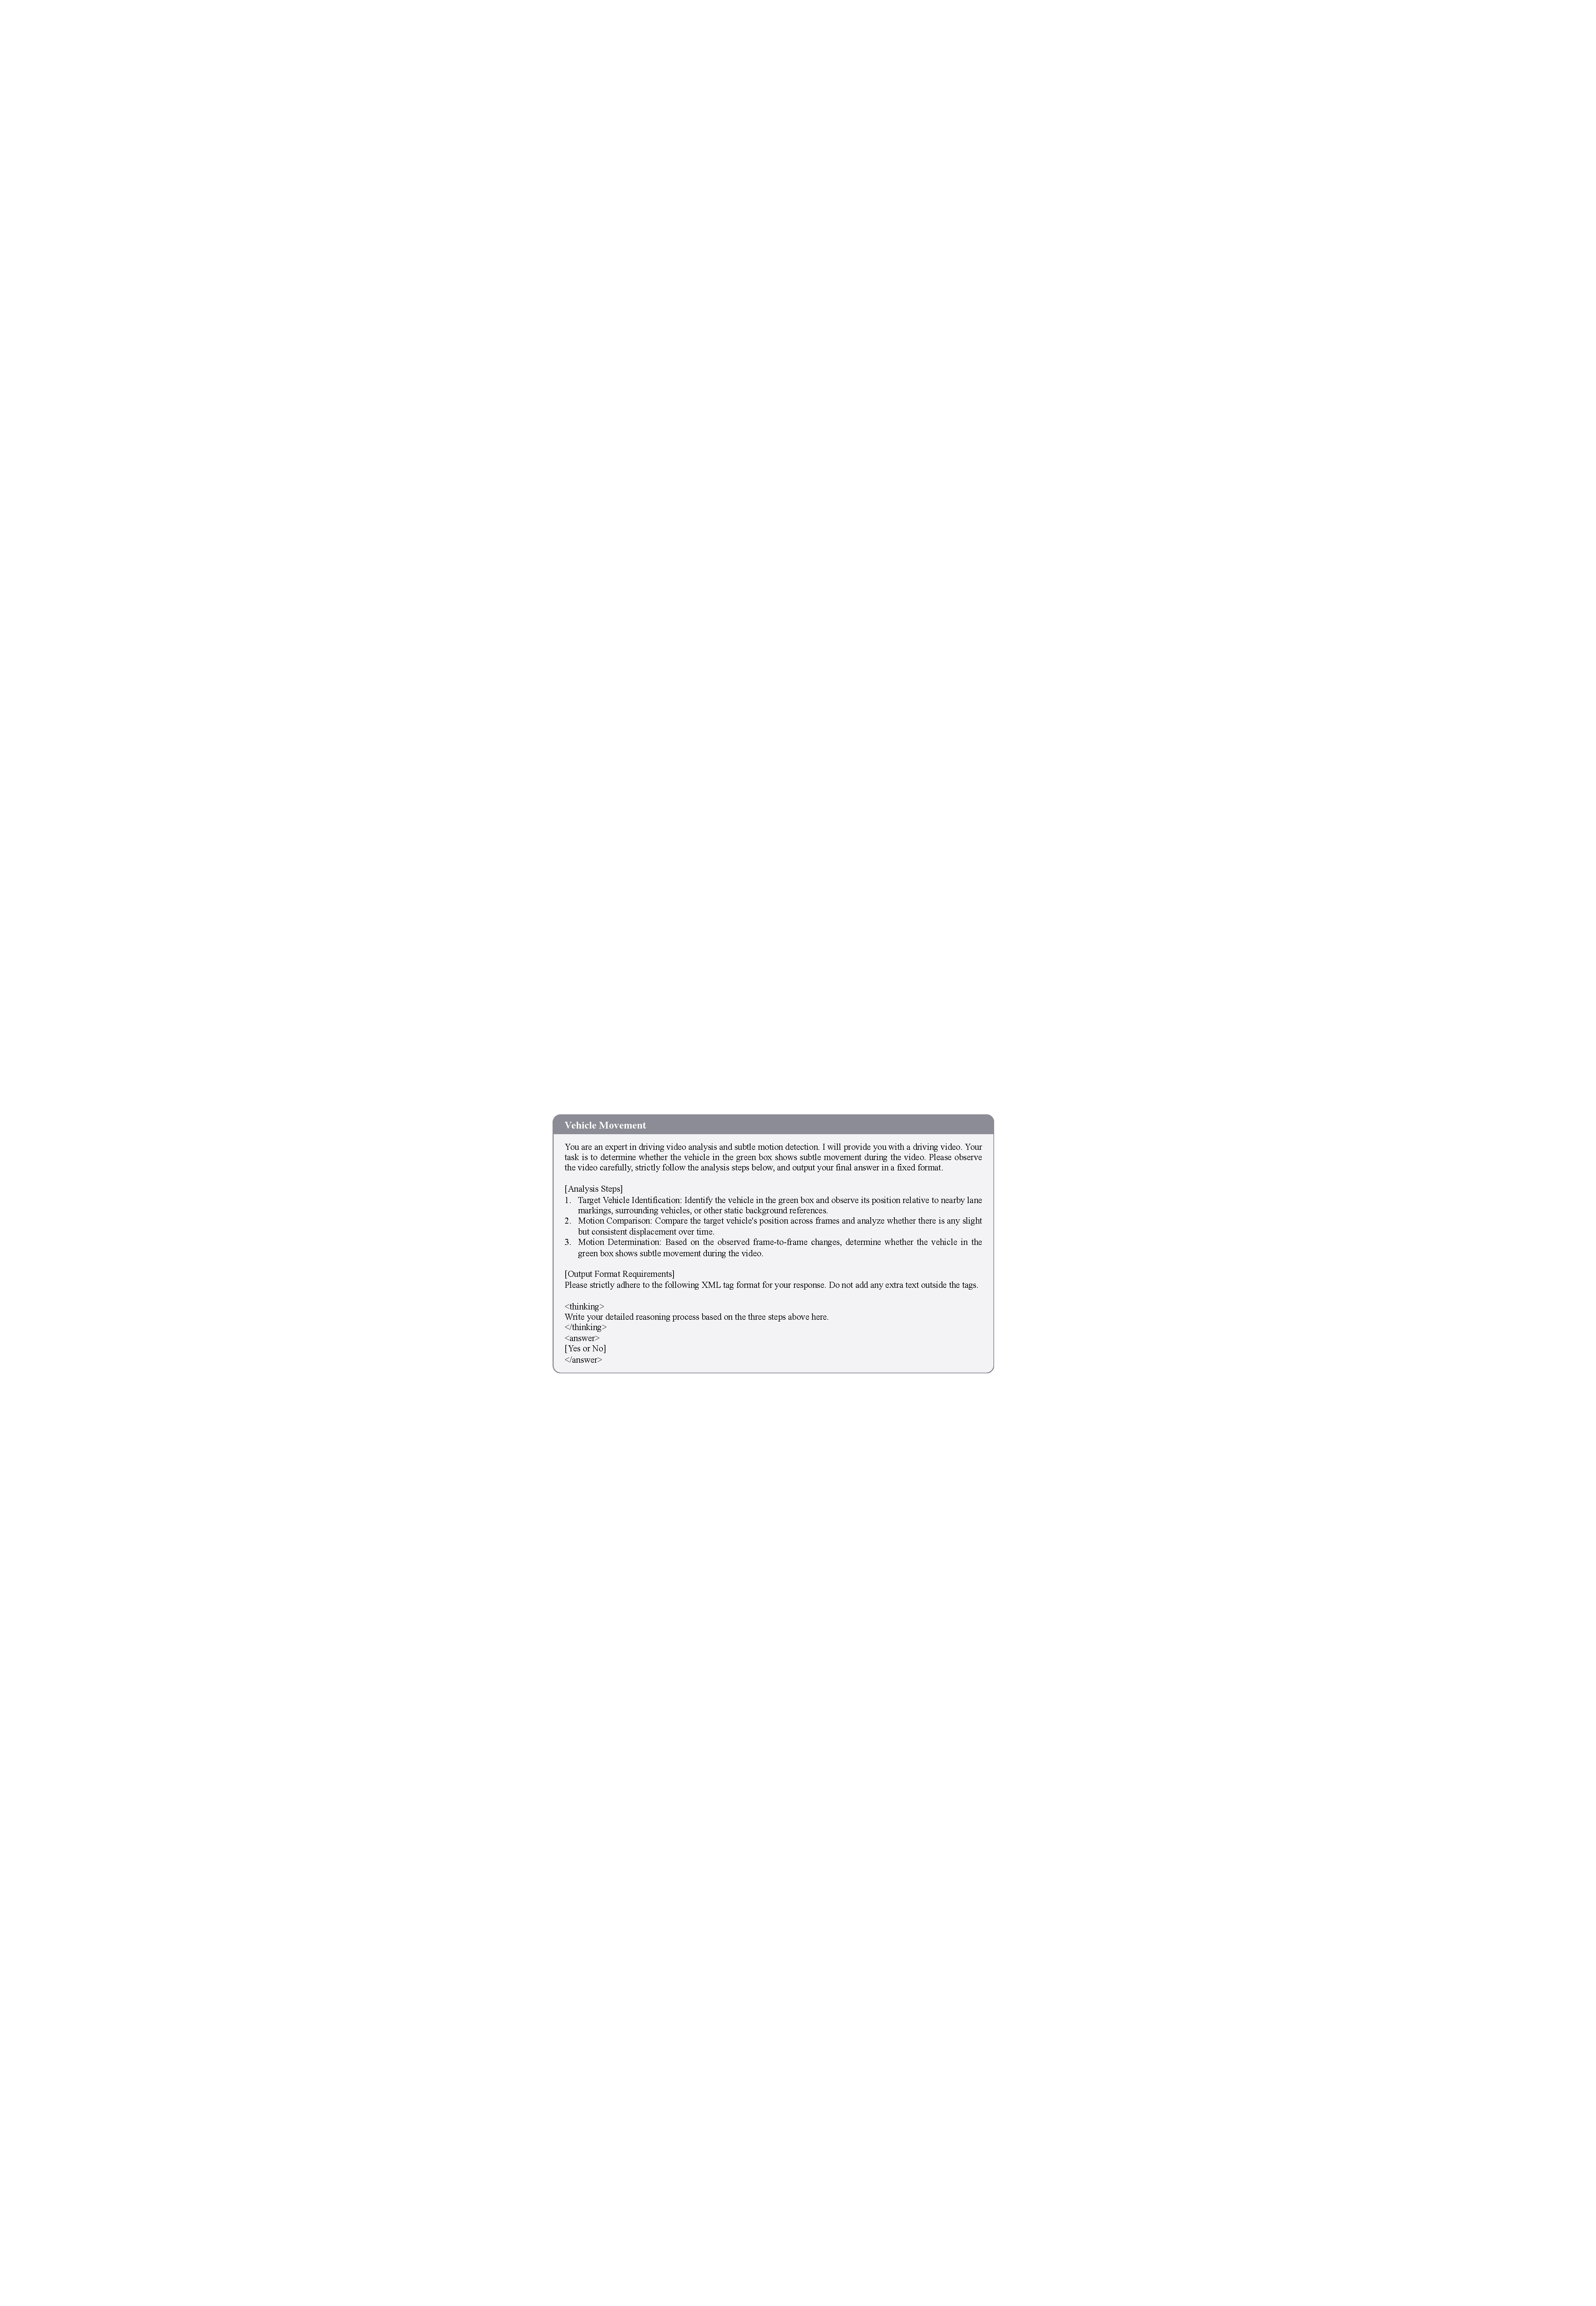
\includegraphics[width=0.95\linewidth]{fig/fig_6.pdf}
  \caption{\textbf{Manual CoT prompt template for Vehicle Movement.}}
  \label{fig:6}
\end{figure}

\begin{figure}[p]
  \centering
  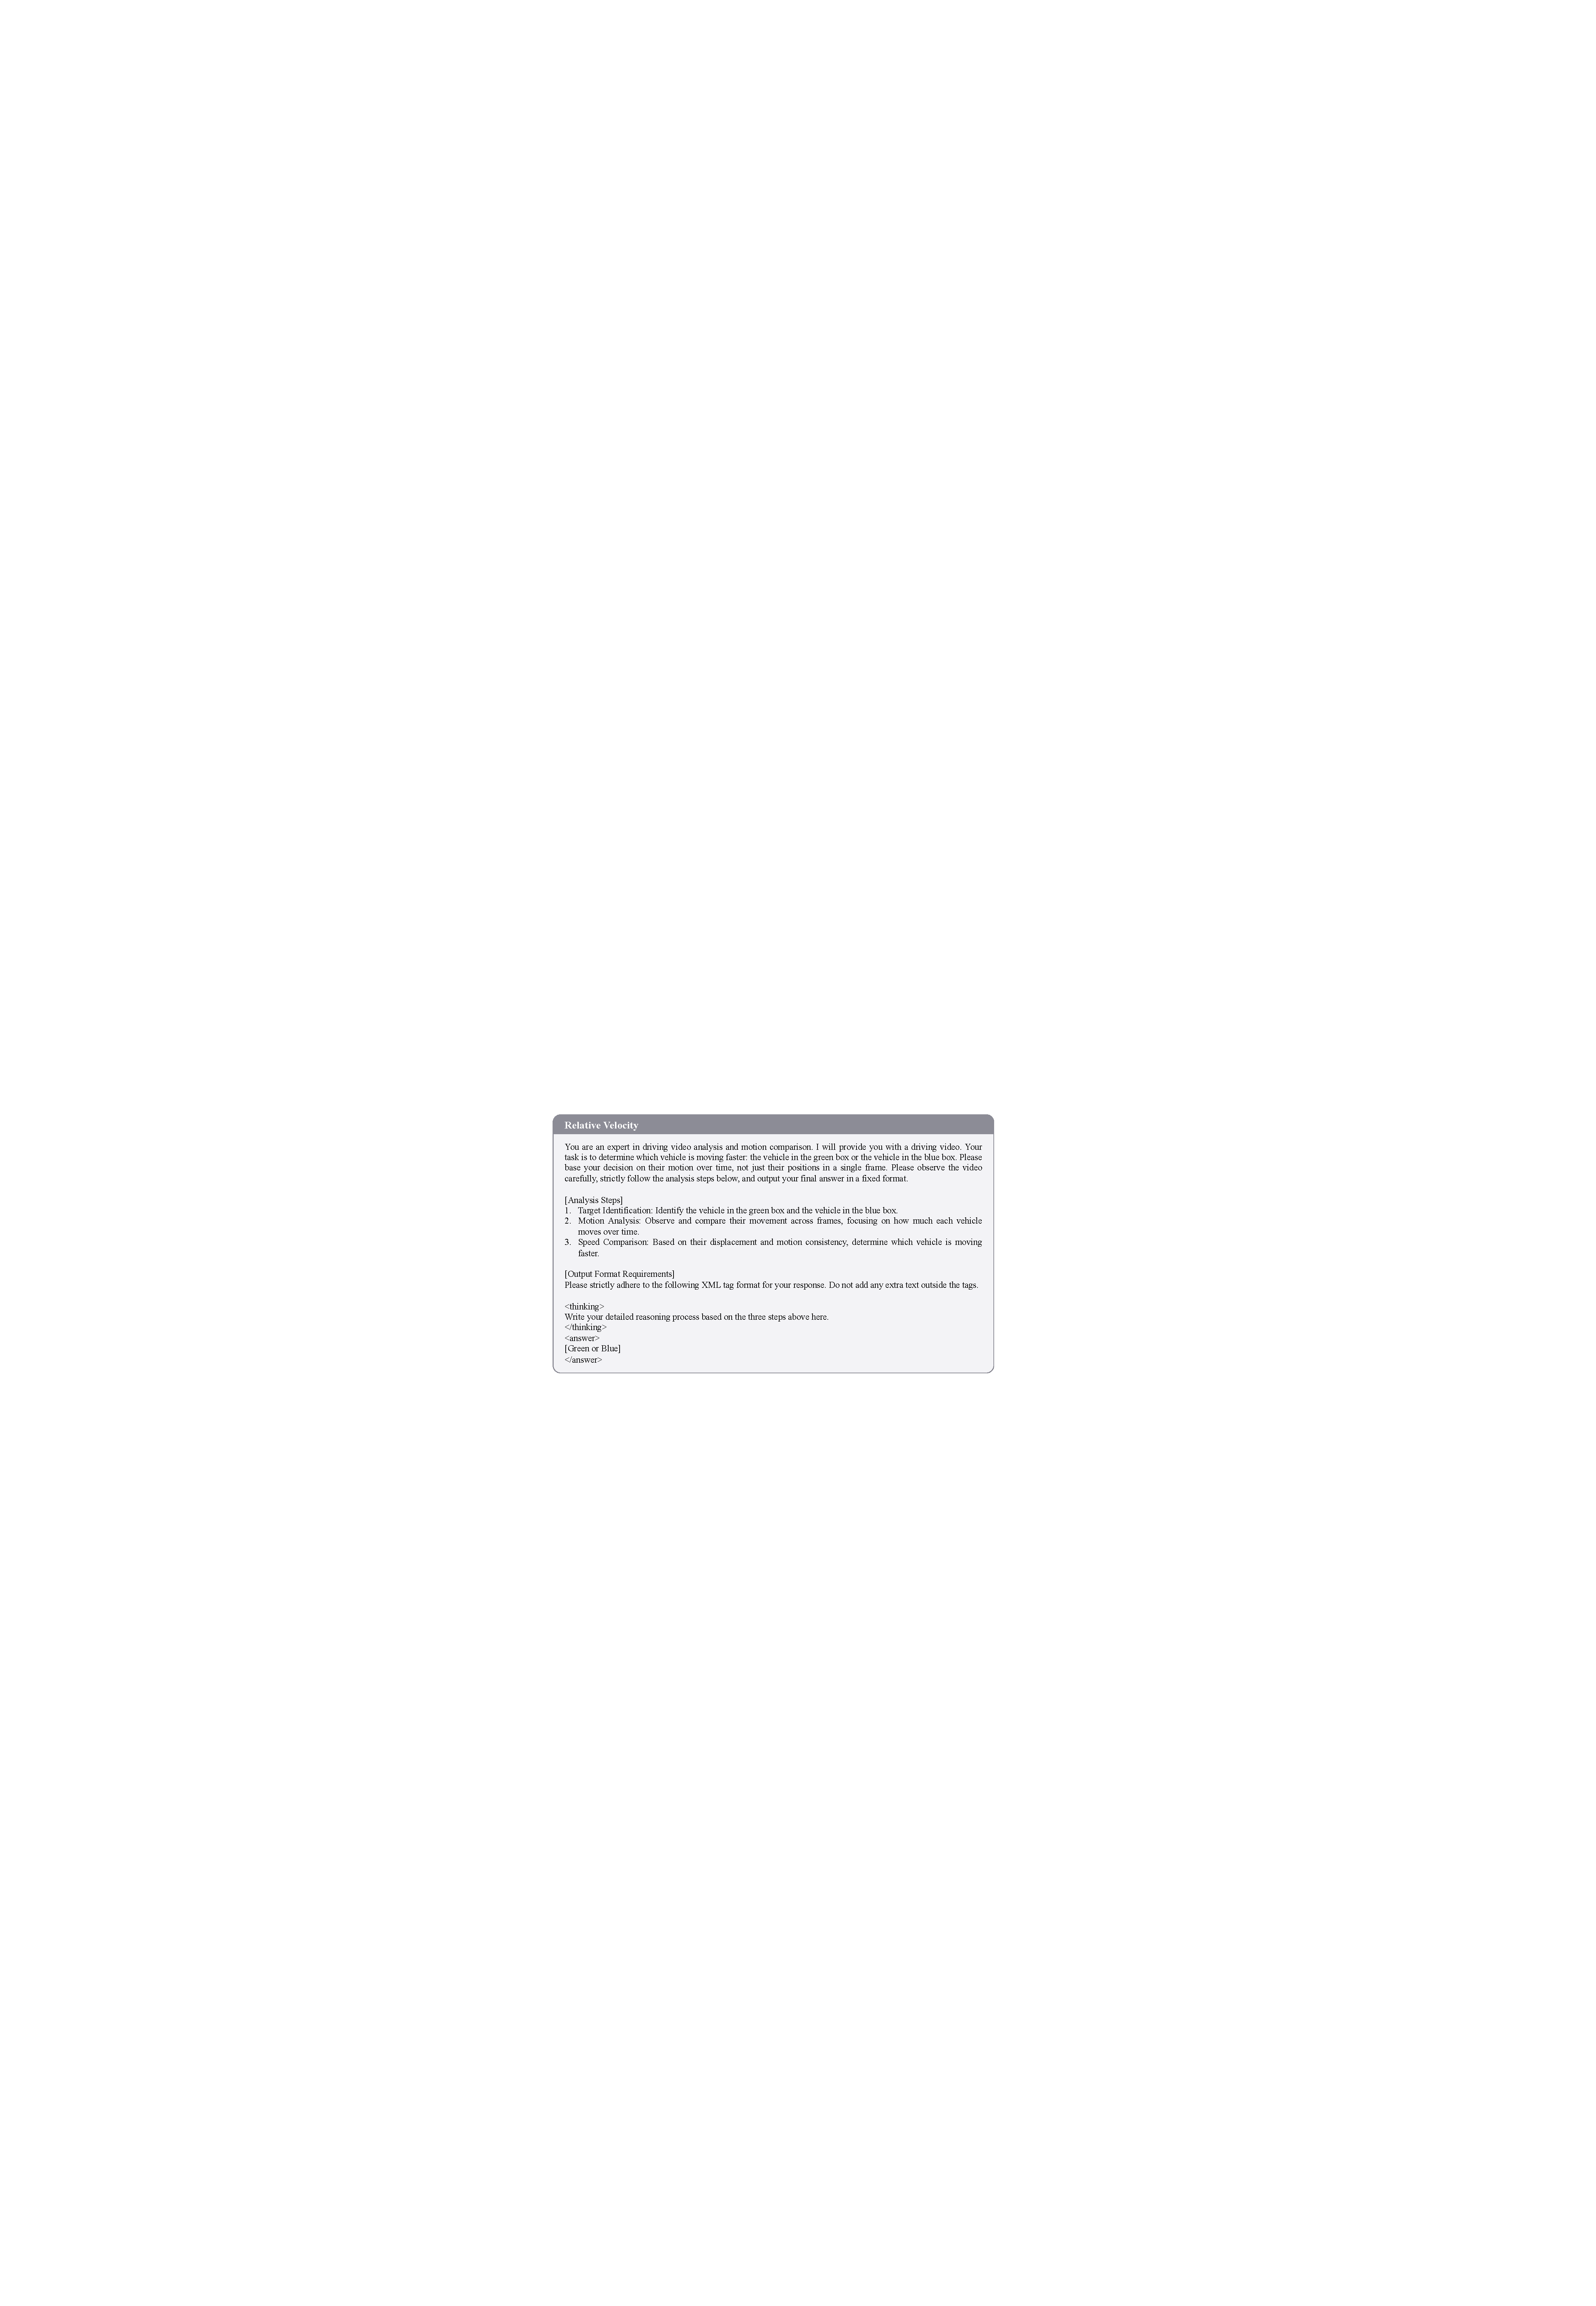
\includegraphics[width=0.95\linewidth]{fig/fig_7.pdf}
  \caption{\textbf{Manual CoT prompt template for Relative Velocity.}}
  \label{fig:7}
\end{figure}

\begin{figure}[p]
  \centering
  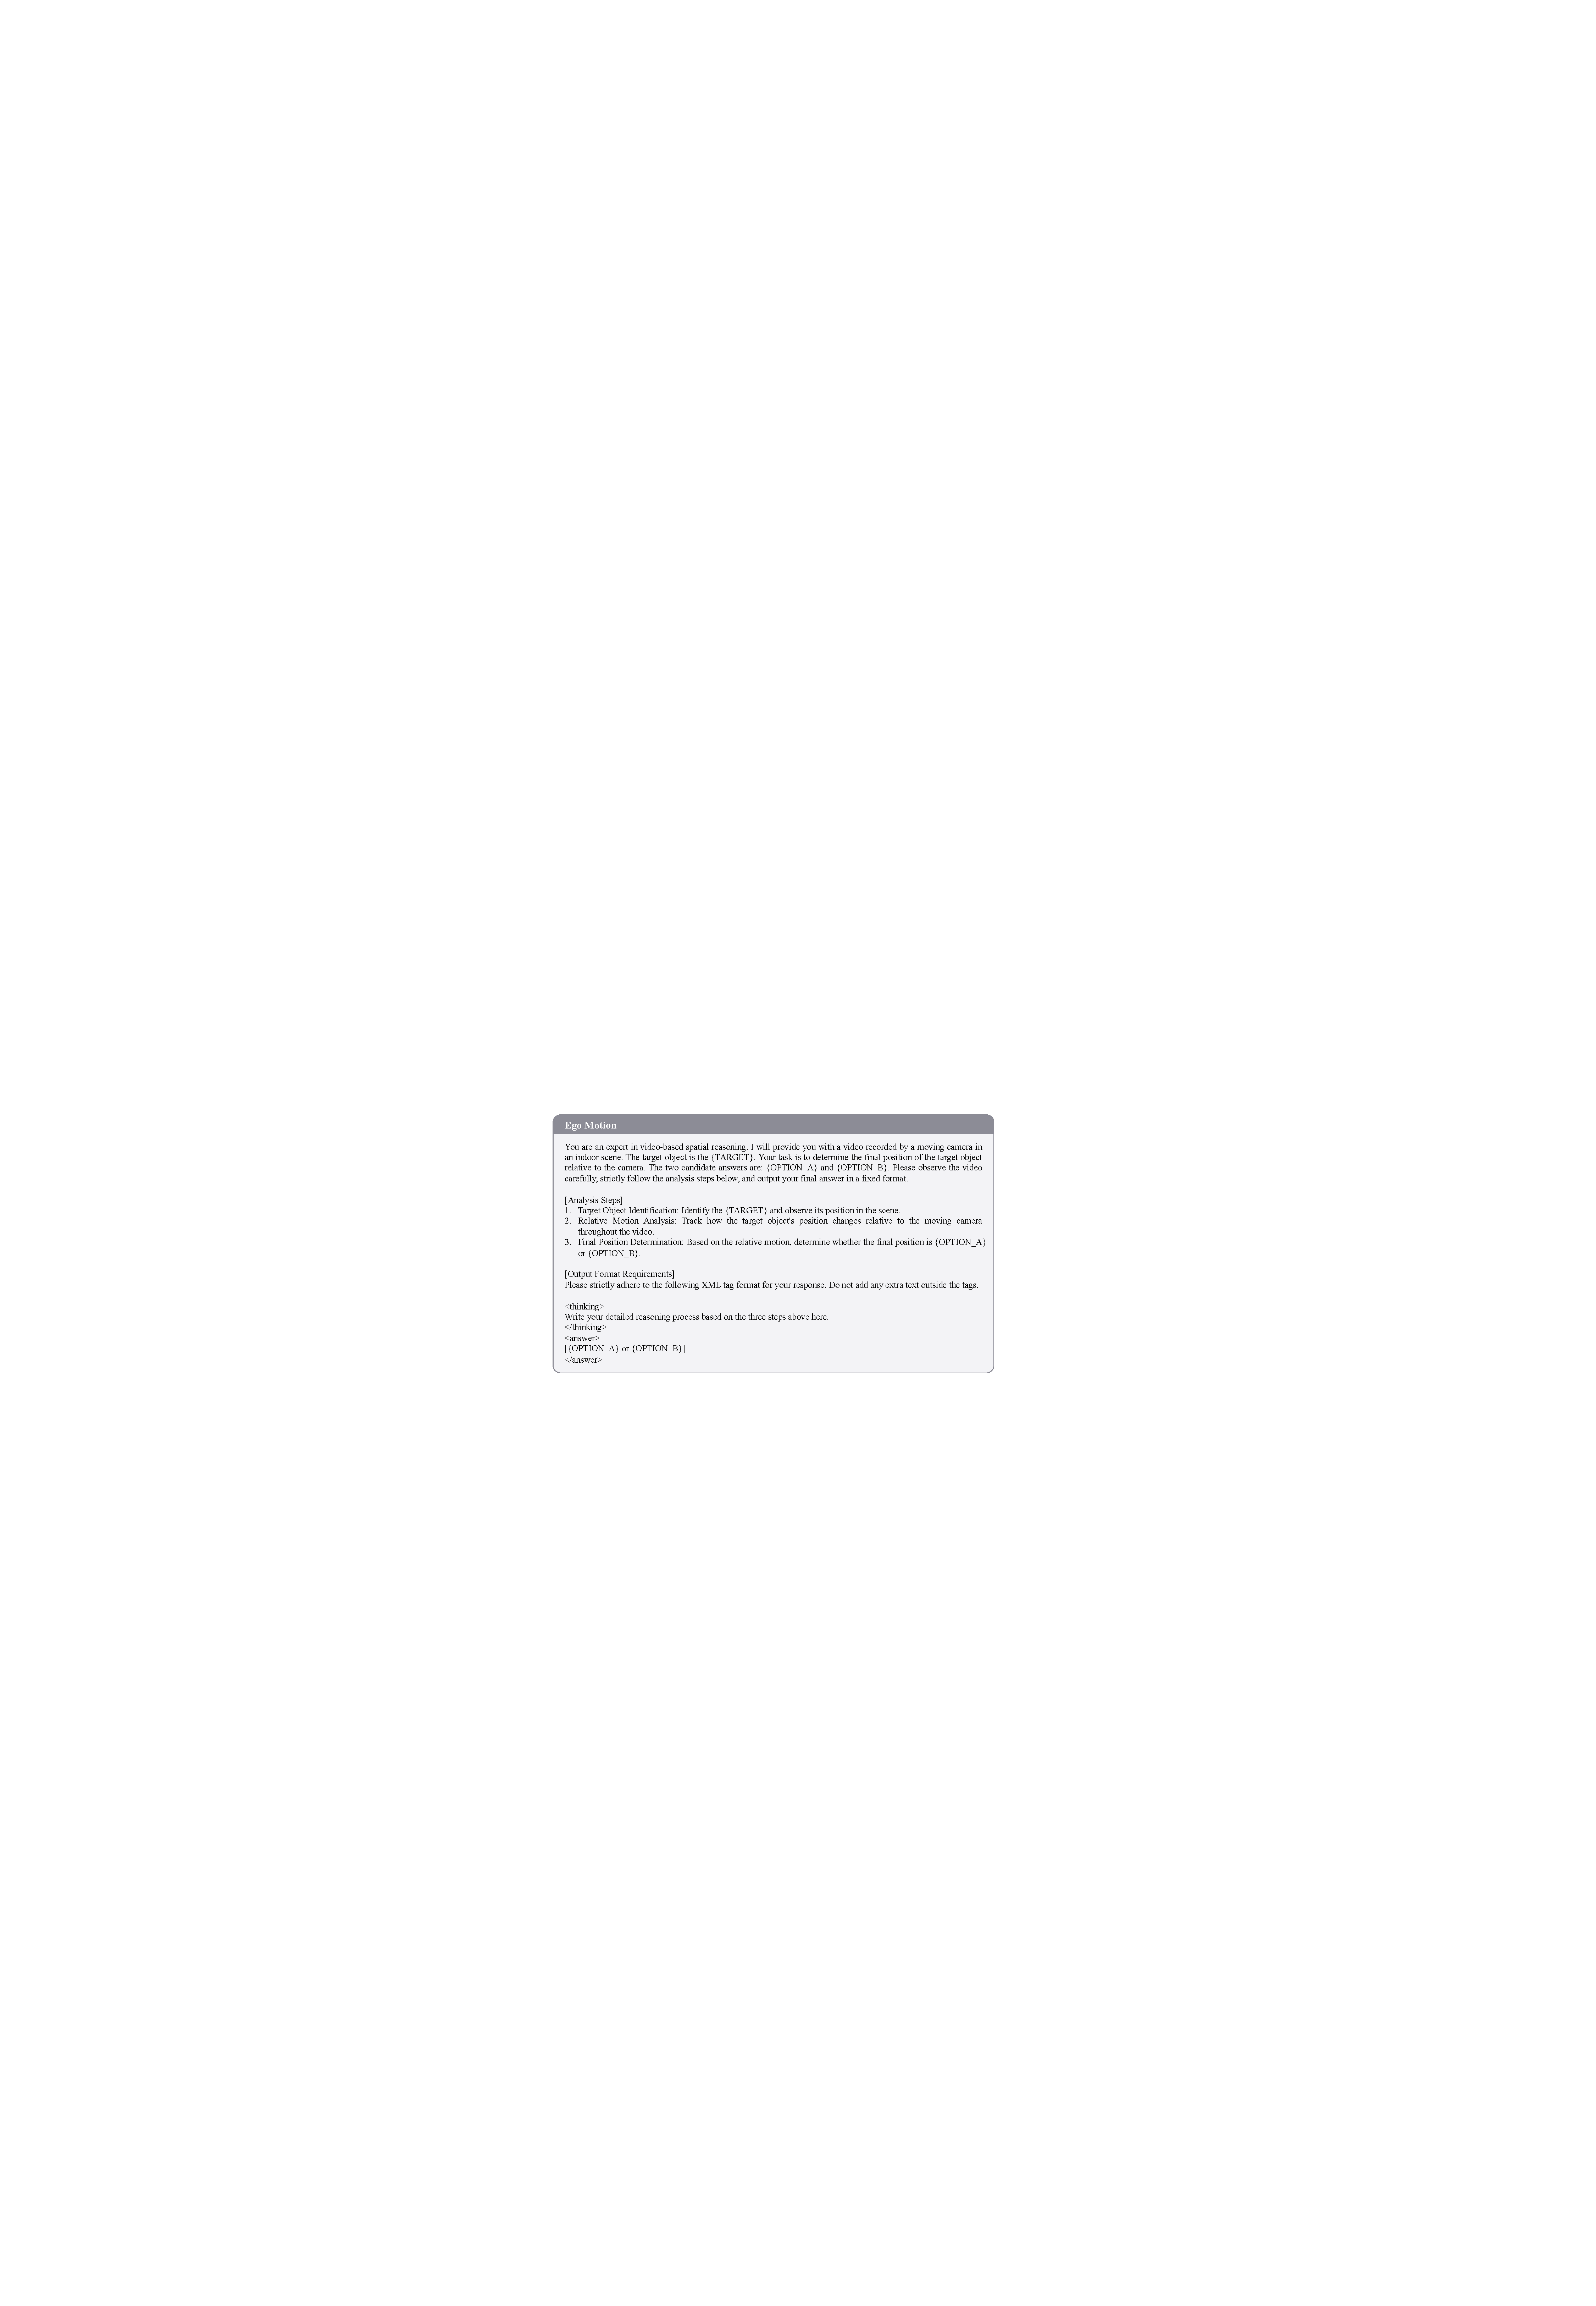
\includegraphics[width=0.95\linewidth]{fig/fig_8.pdf}
  \caption{\textbf{Manual CoT prompt template for Ego Motion.}}
  \label{fig:8}
\end{figure}

\begin{figure}[p]
  \centering
  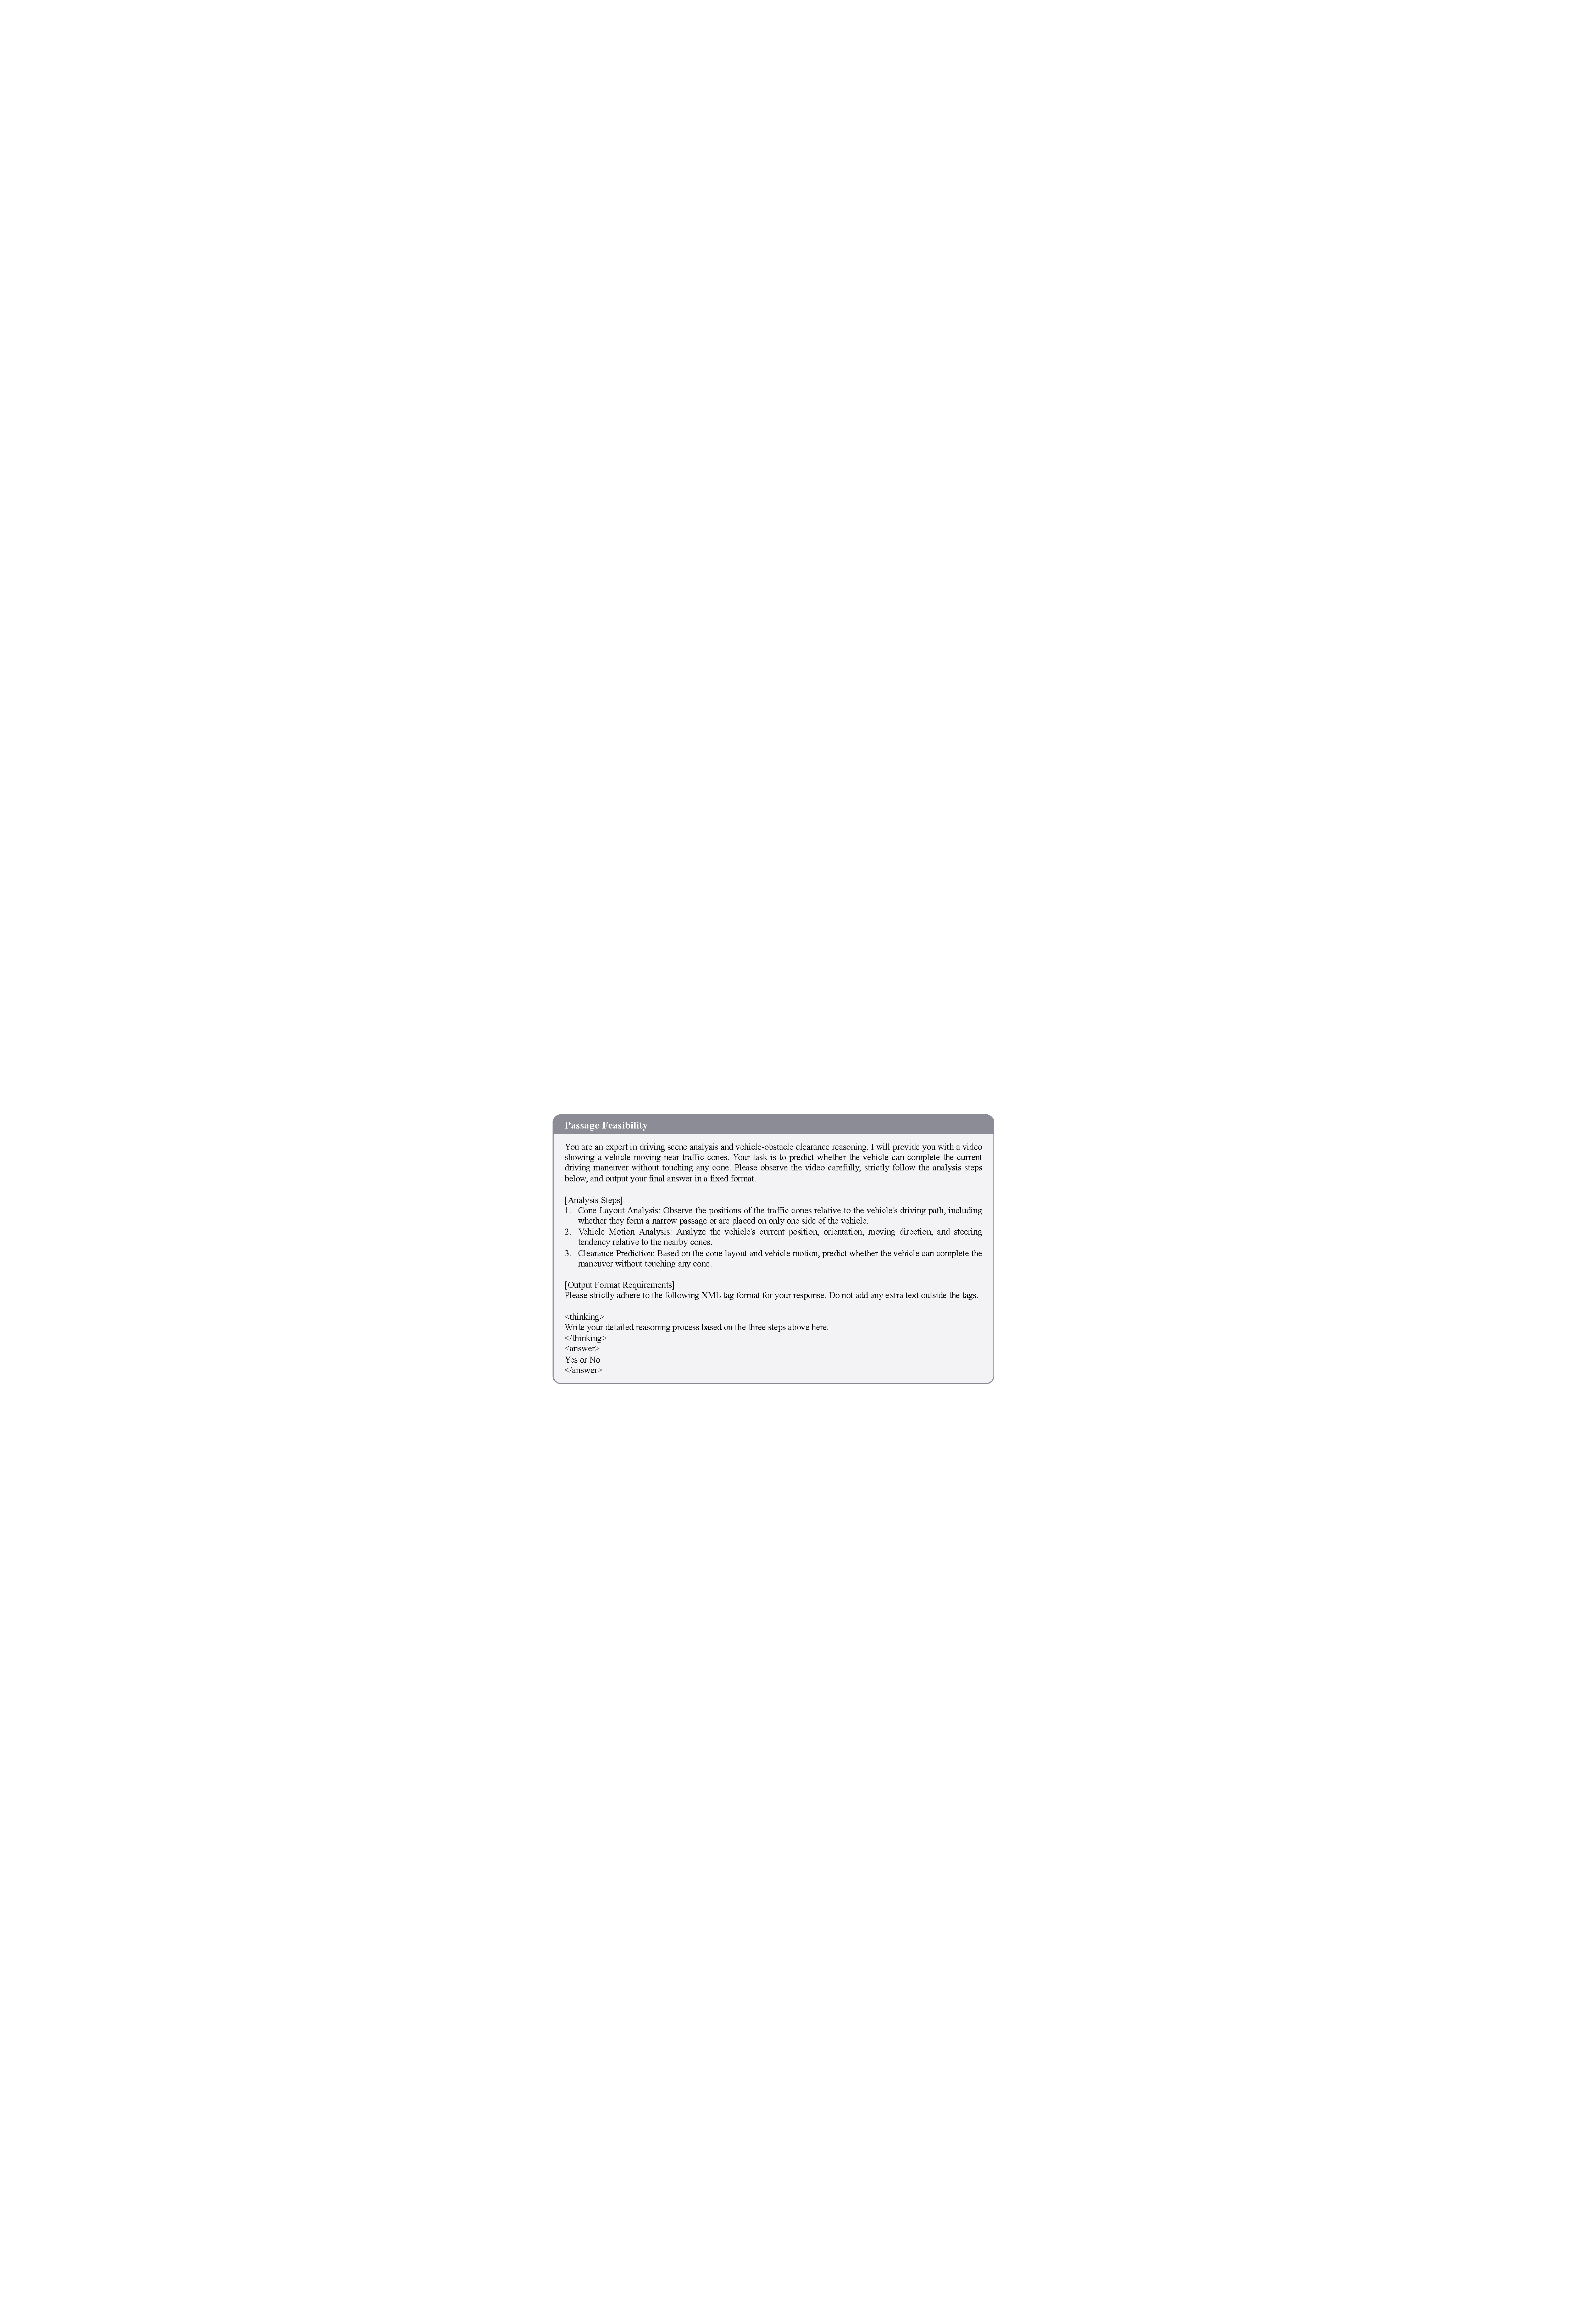
\includegraphics[width=0.95\linewidth]{fig/fig_9.pdf}
  \caption{\textbf{Manual CoT prompt template for Passage Feasibility.}}
  \label{fig:9}
\end{figure}

\begin{figure}[p]
  \centering
  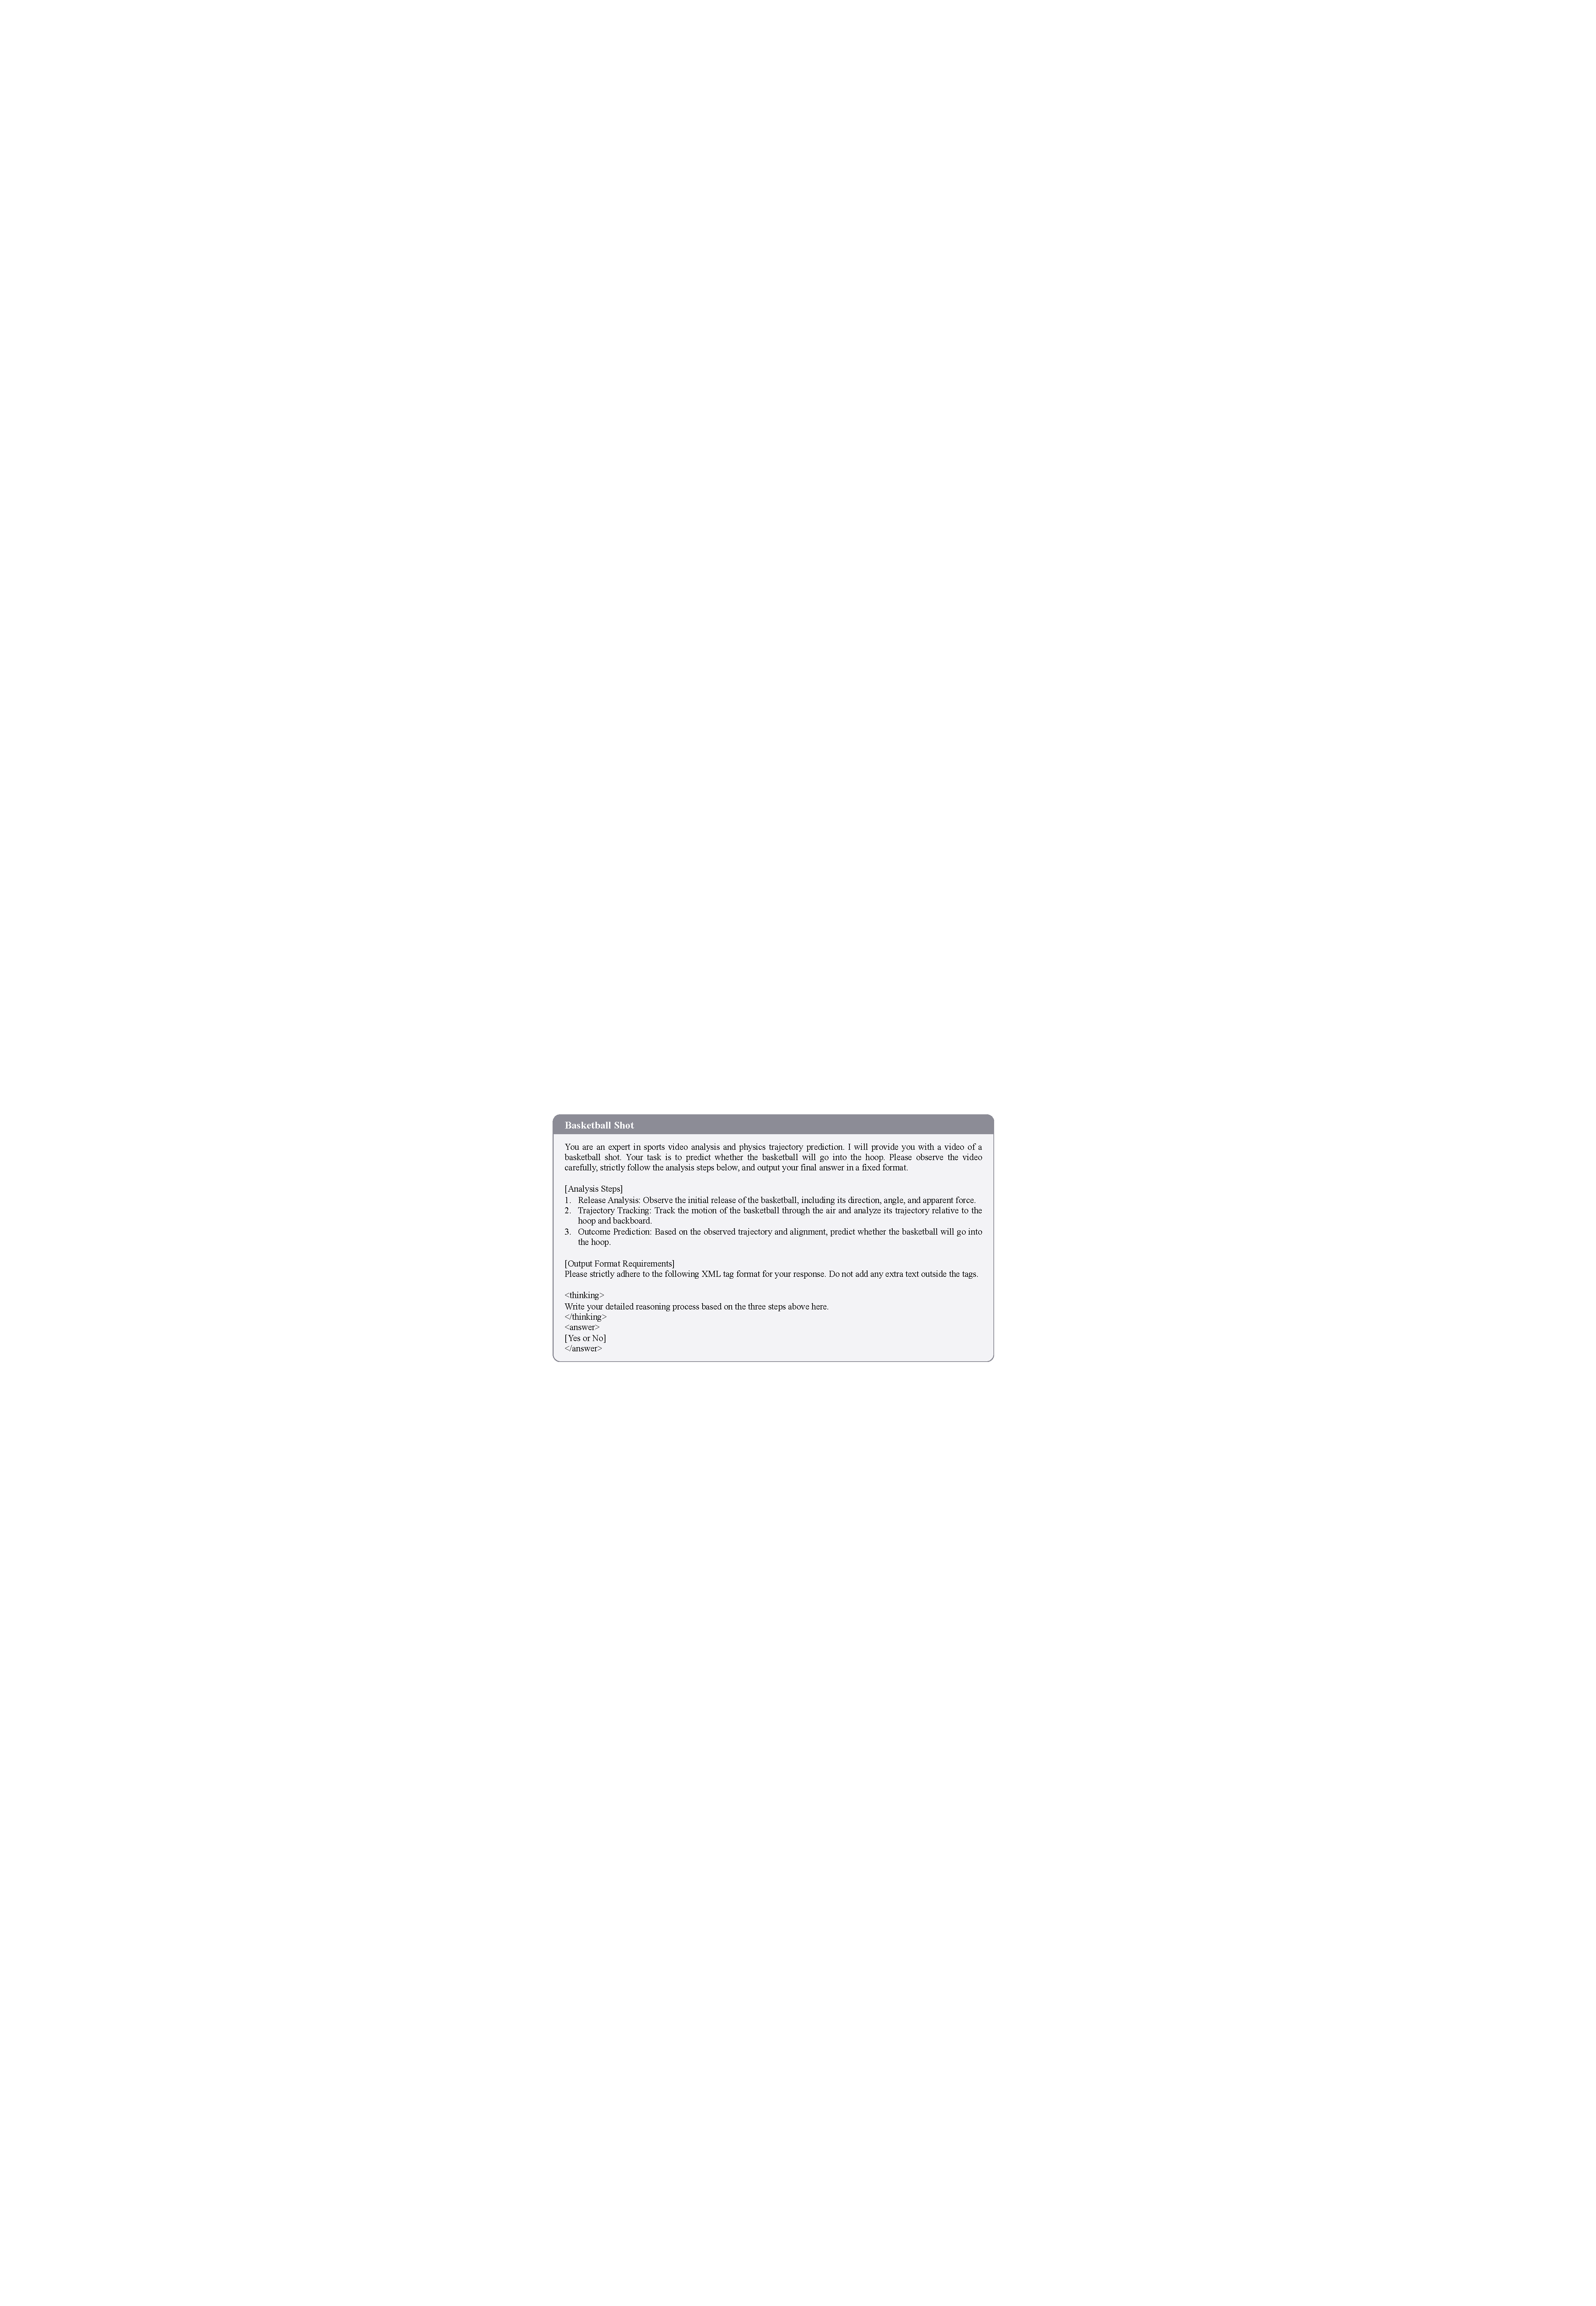
\includegraphics[width=0.95\linewidth]{fig/fig_10.pdf}
  \caption{\textbf{Manual CoT prompt template for Basketball Shot.}}
  \label{fig:10}
\end{figure}

\begin{figure}[p]
  \centering
  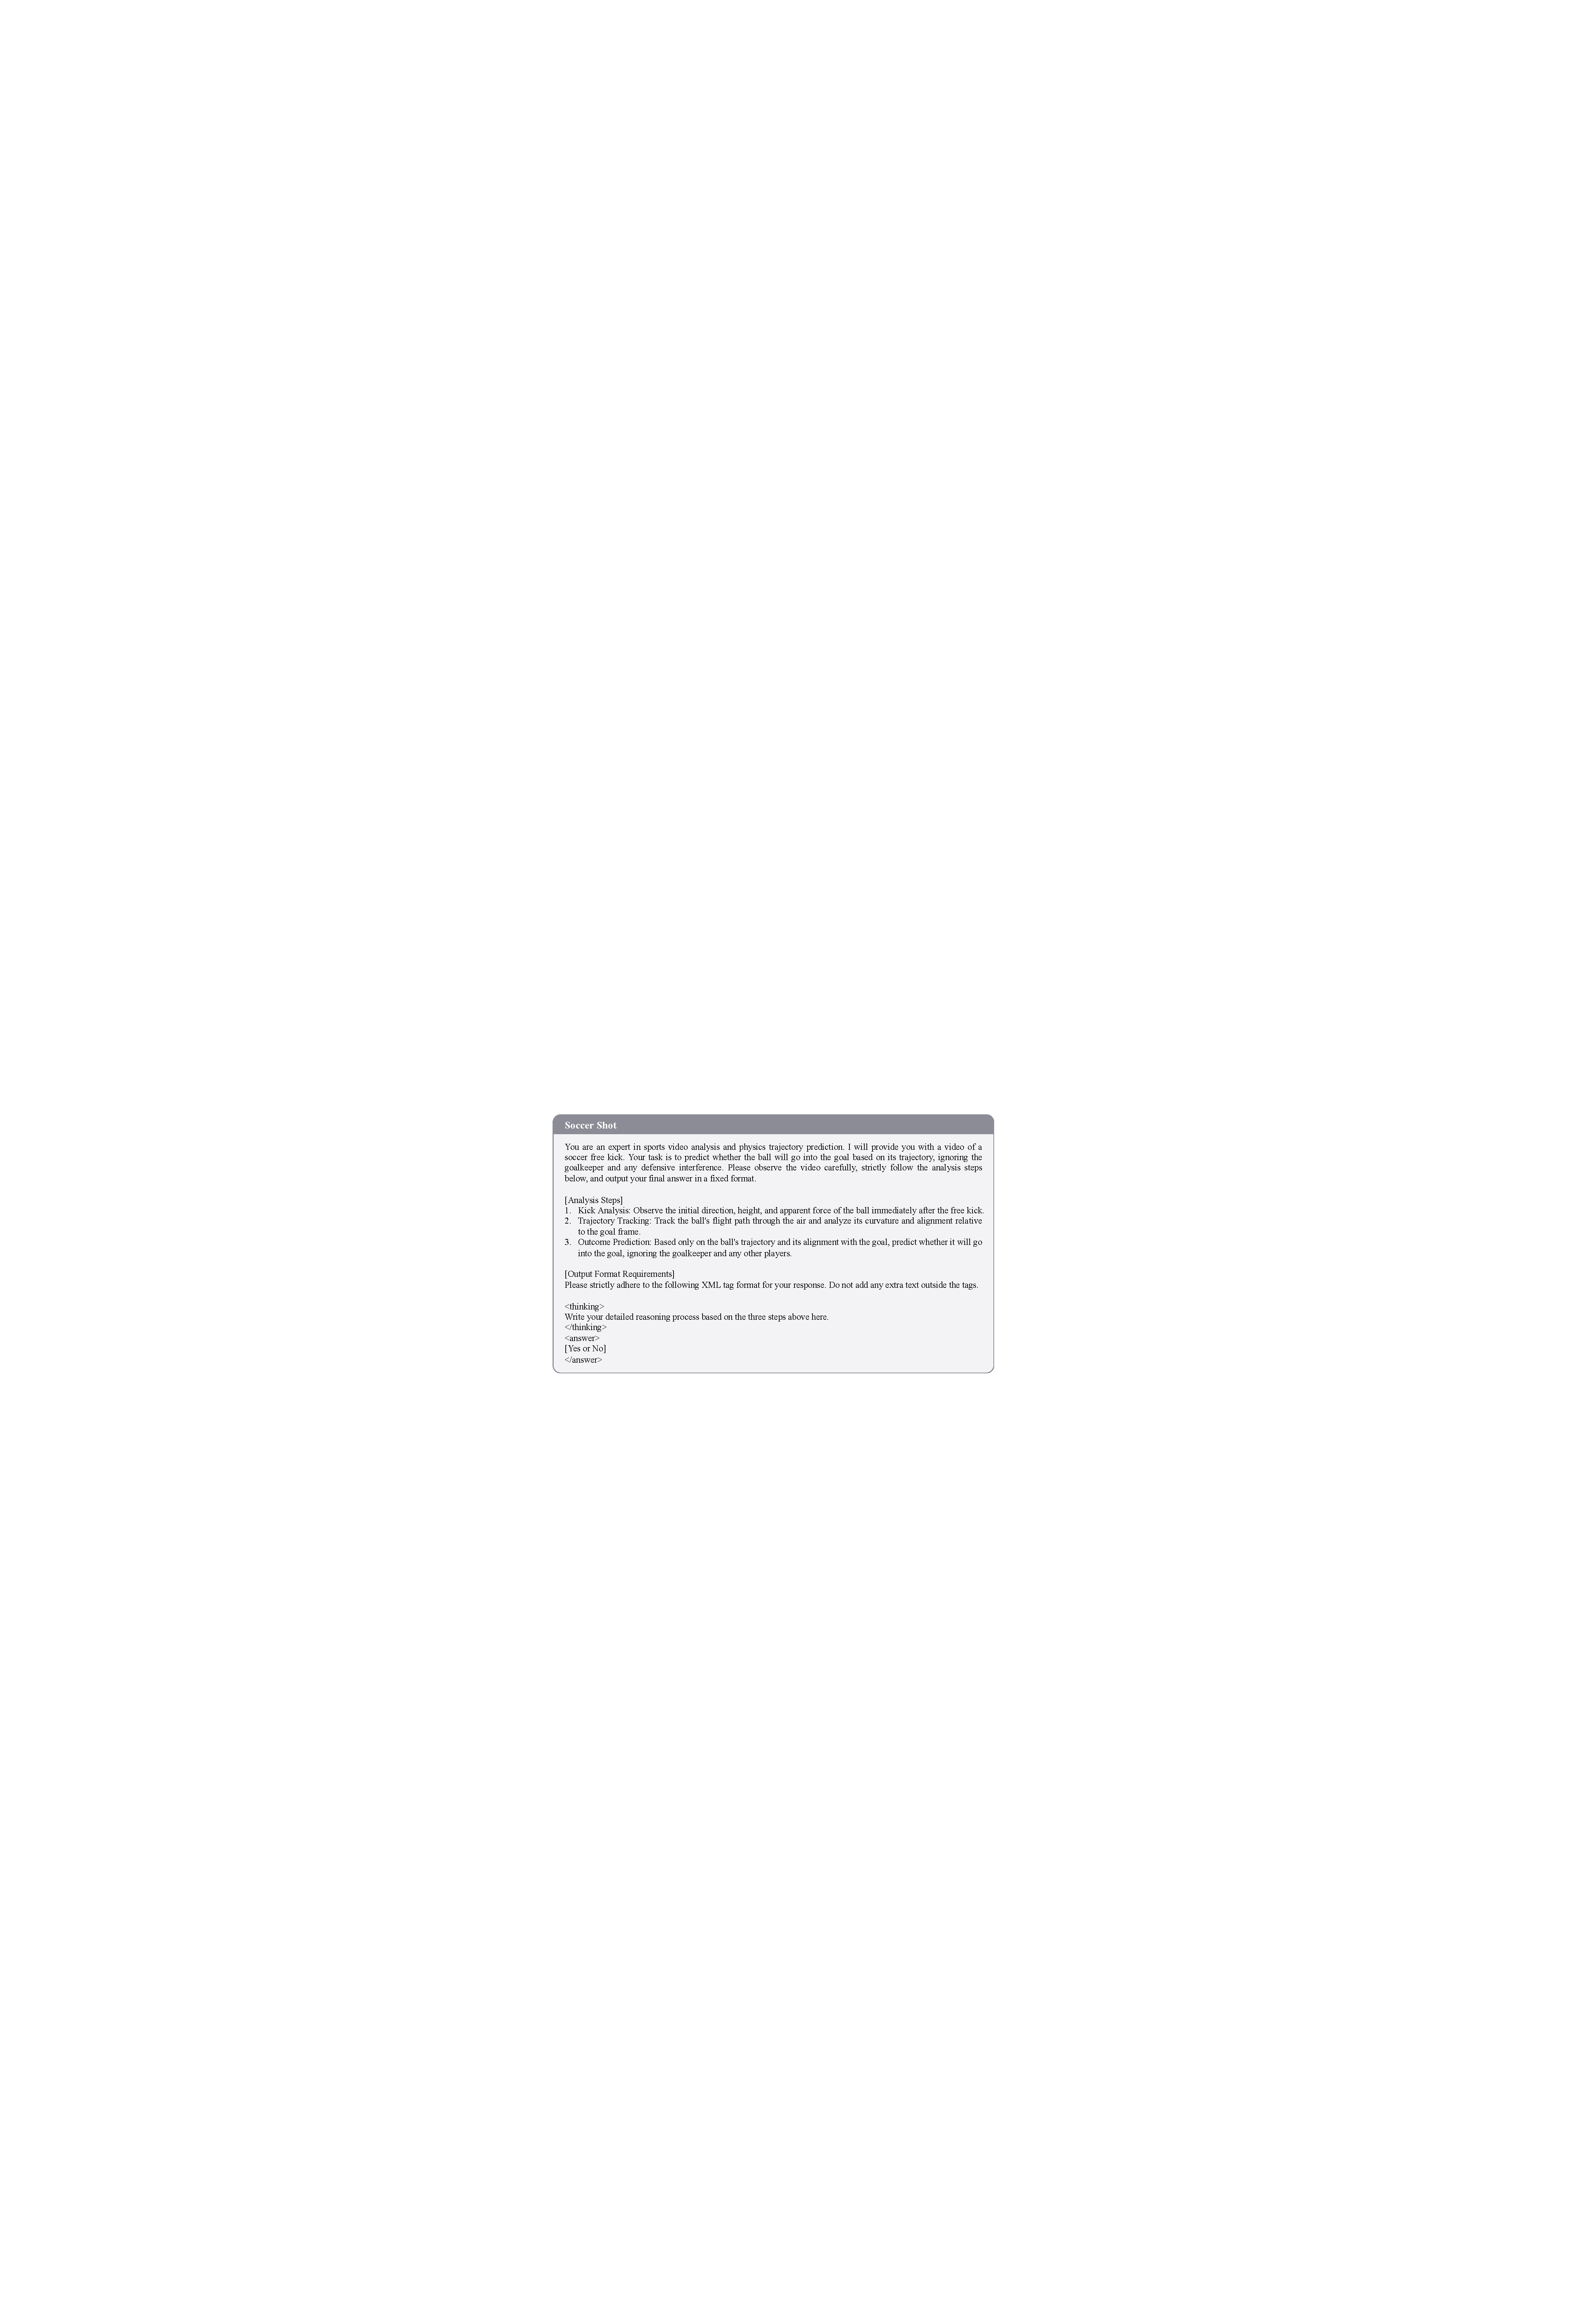
\includegraphics[width=0.95\linewidth]{fig/fig_11.pdf}
  \caption{\textbf{Manual CoT prompt template for Soccer Shot.}}
  \label{fig:11}
\end{figure}

\begin{figure}[p]
  \centering
  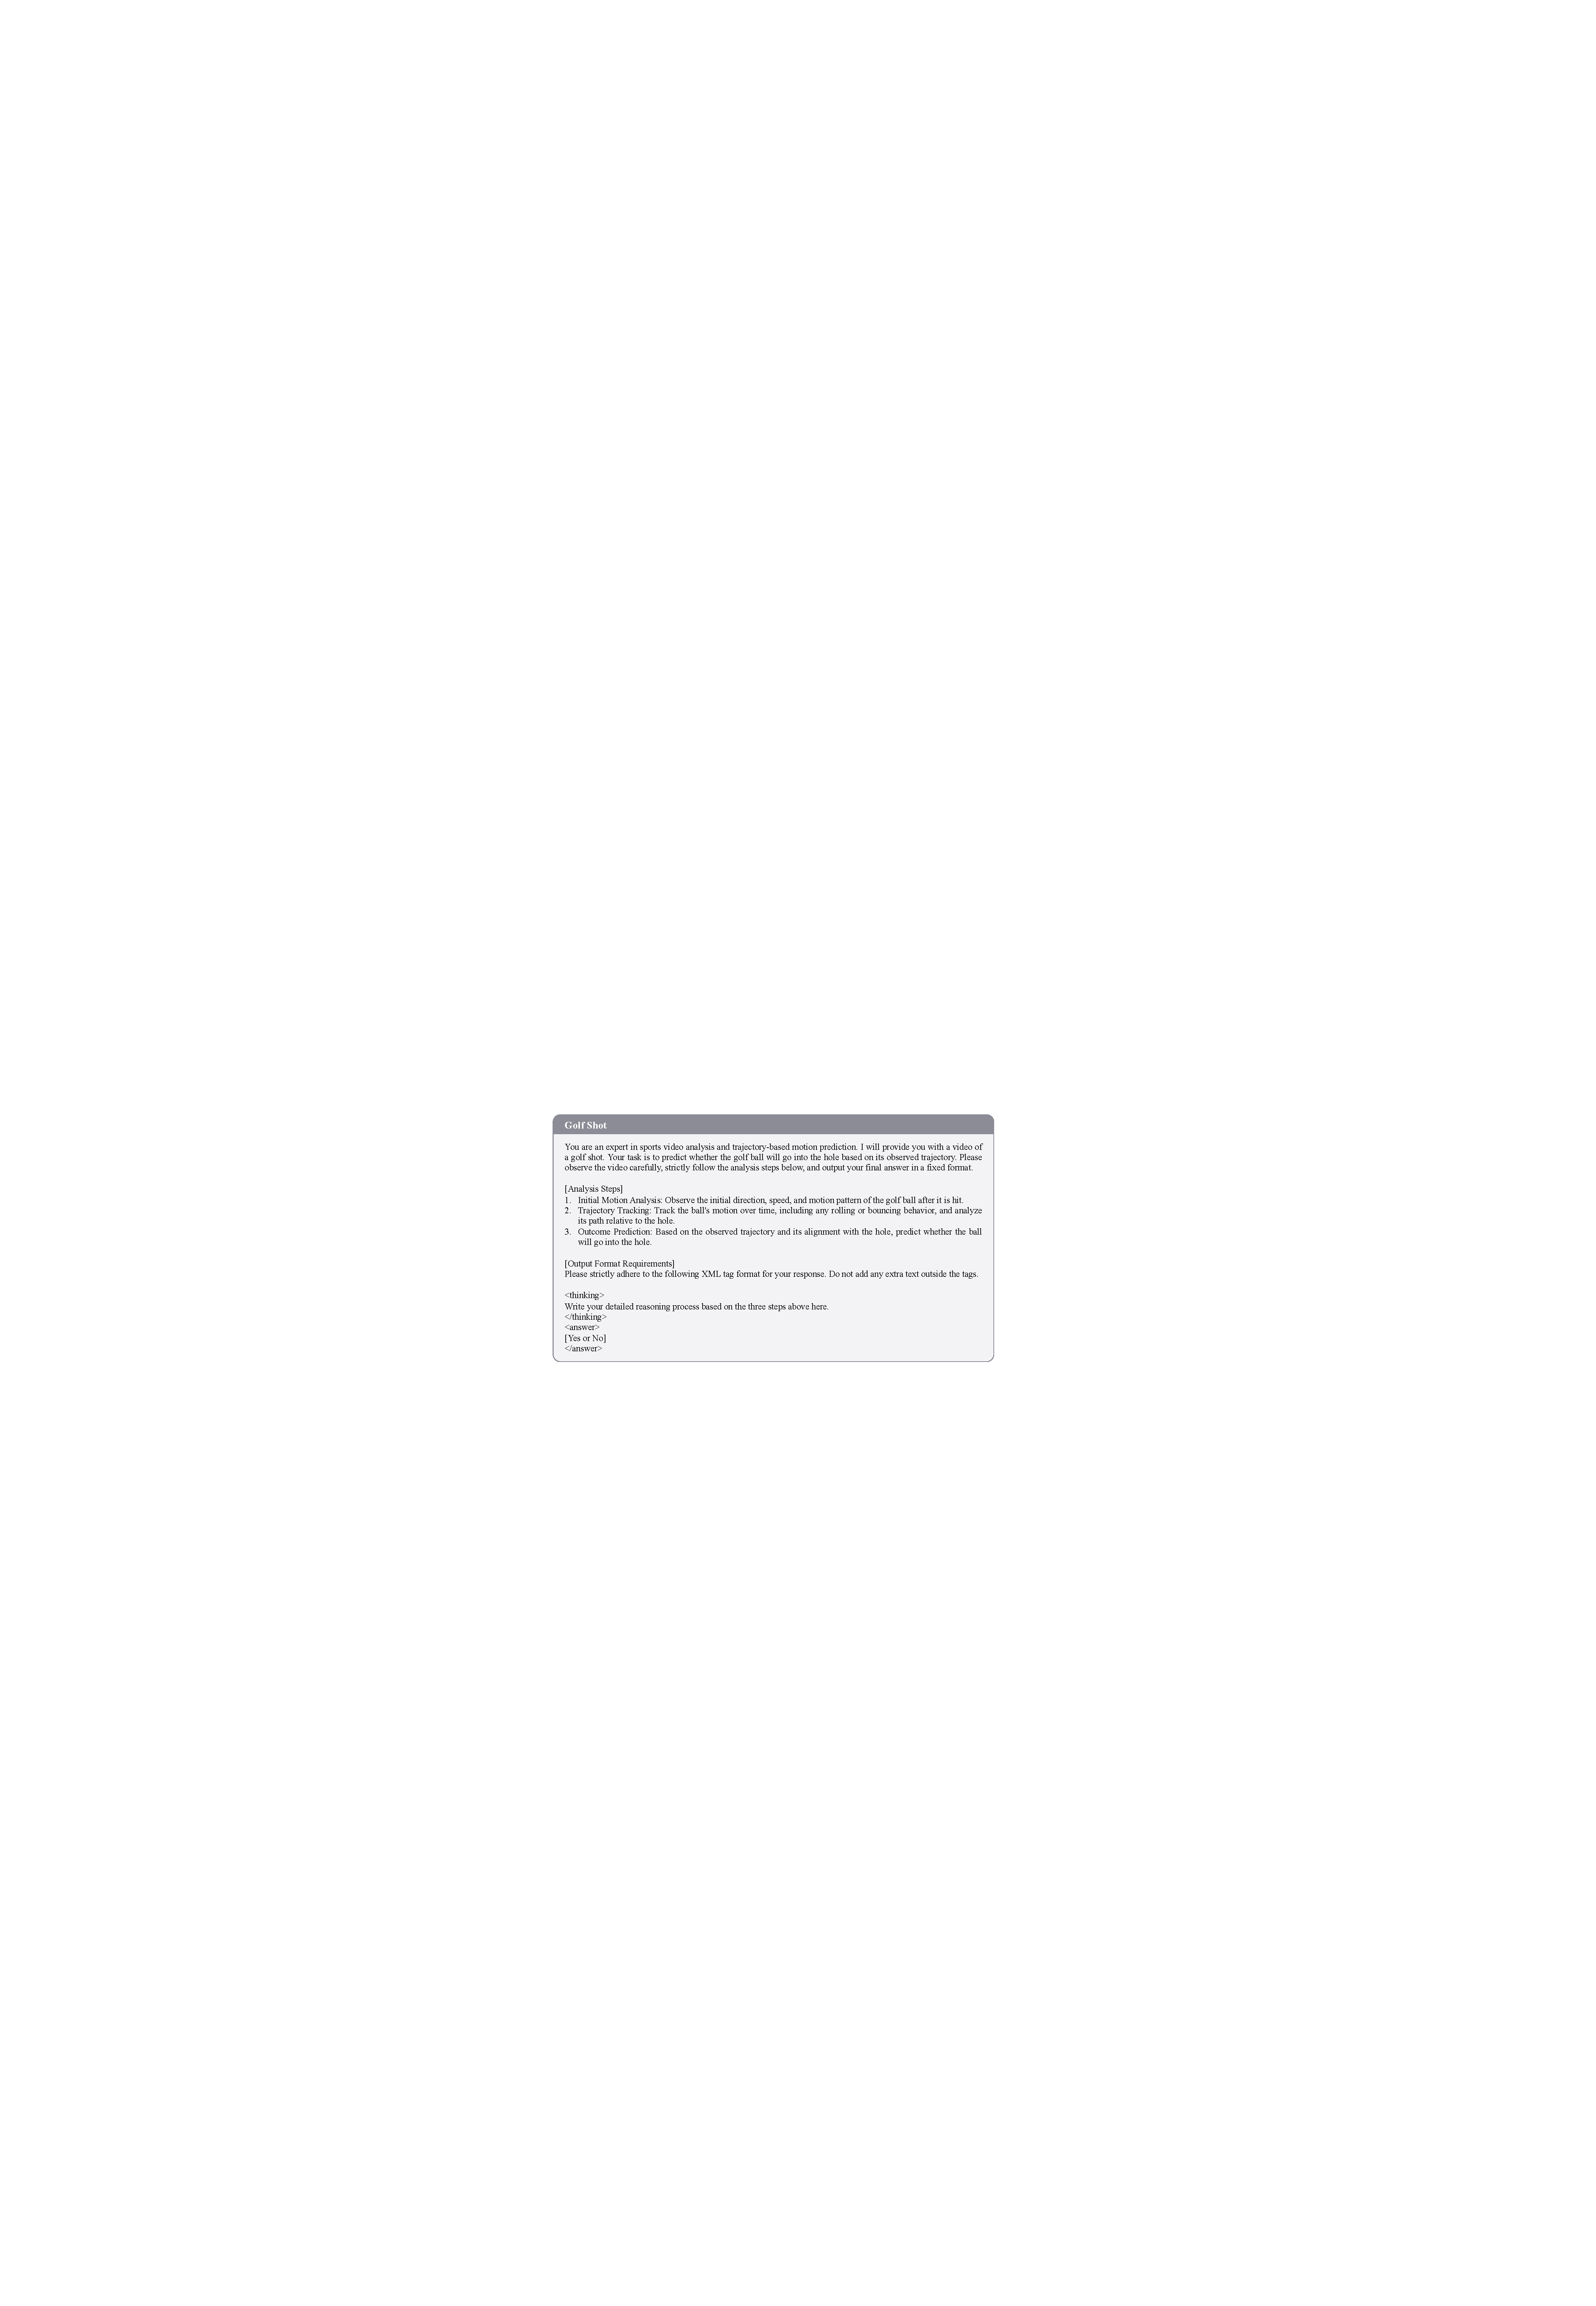
\includegraphics[width=0.95\linewidth]{fig/fig_12.pdf}
  \caption{\textbf{Manual CoT prompt template for Golf Shot.}}
  \label{fig:12}
\end{figure}

\begin{figure}[p]
  \centering
  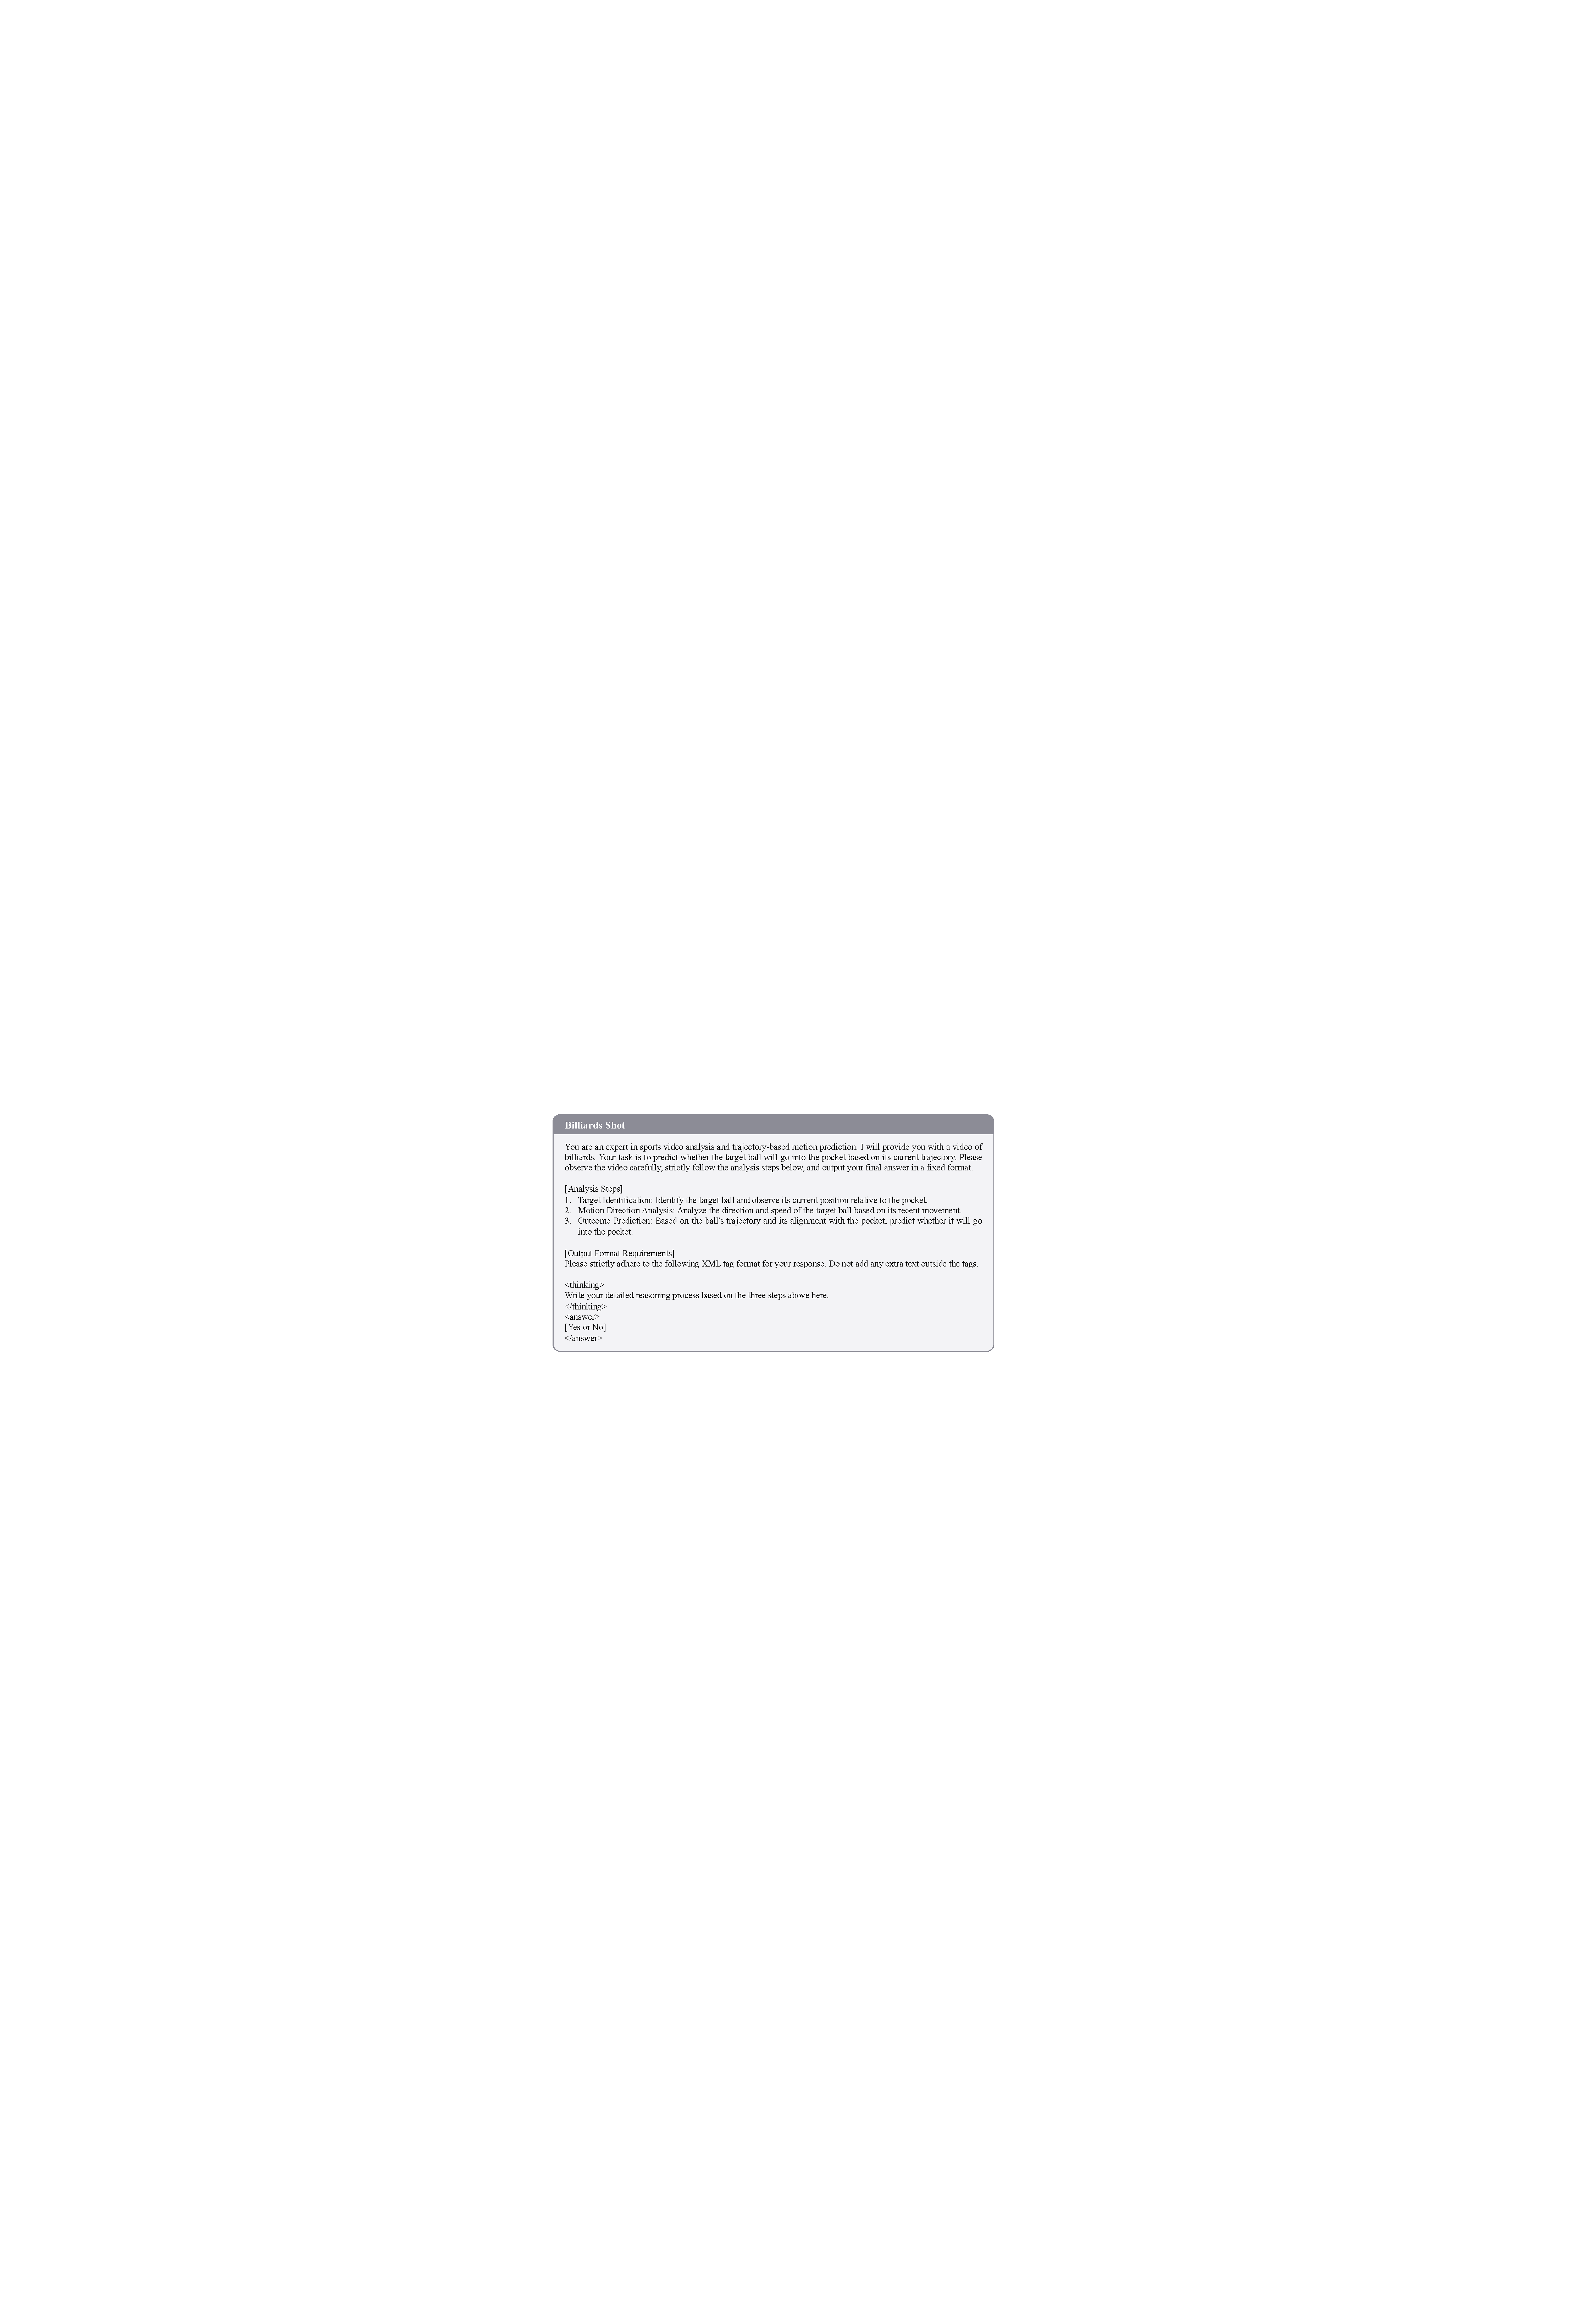
\includegraphics[width=0.95\linewidth]{fig/fig_13.pdf}
  \caption{\textbf{Manual CoT prompt template for Billiards Shot.}}
  \label{fig:13}
\end{figure}

\begin{figure}[p]
  \centering
  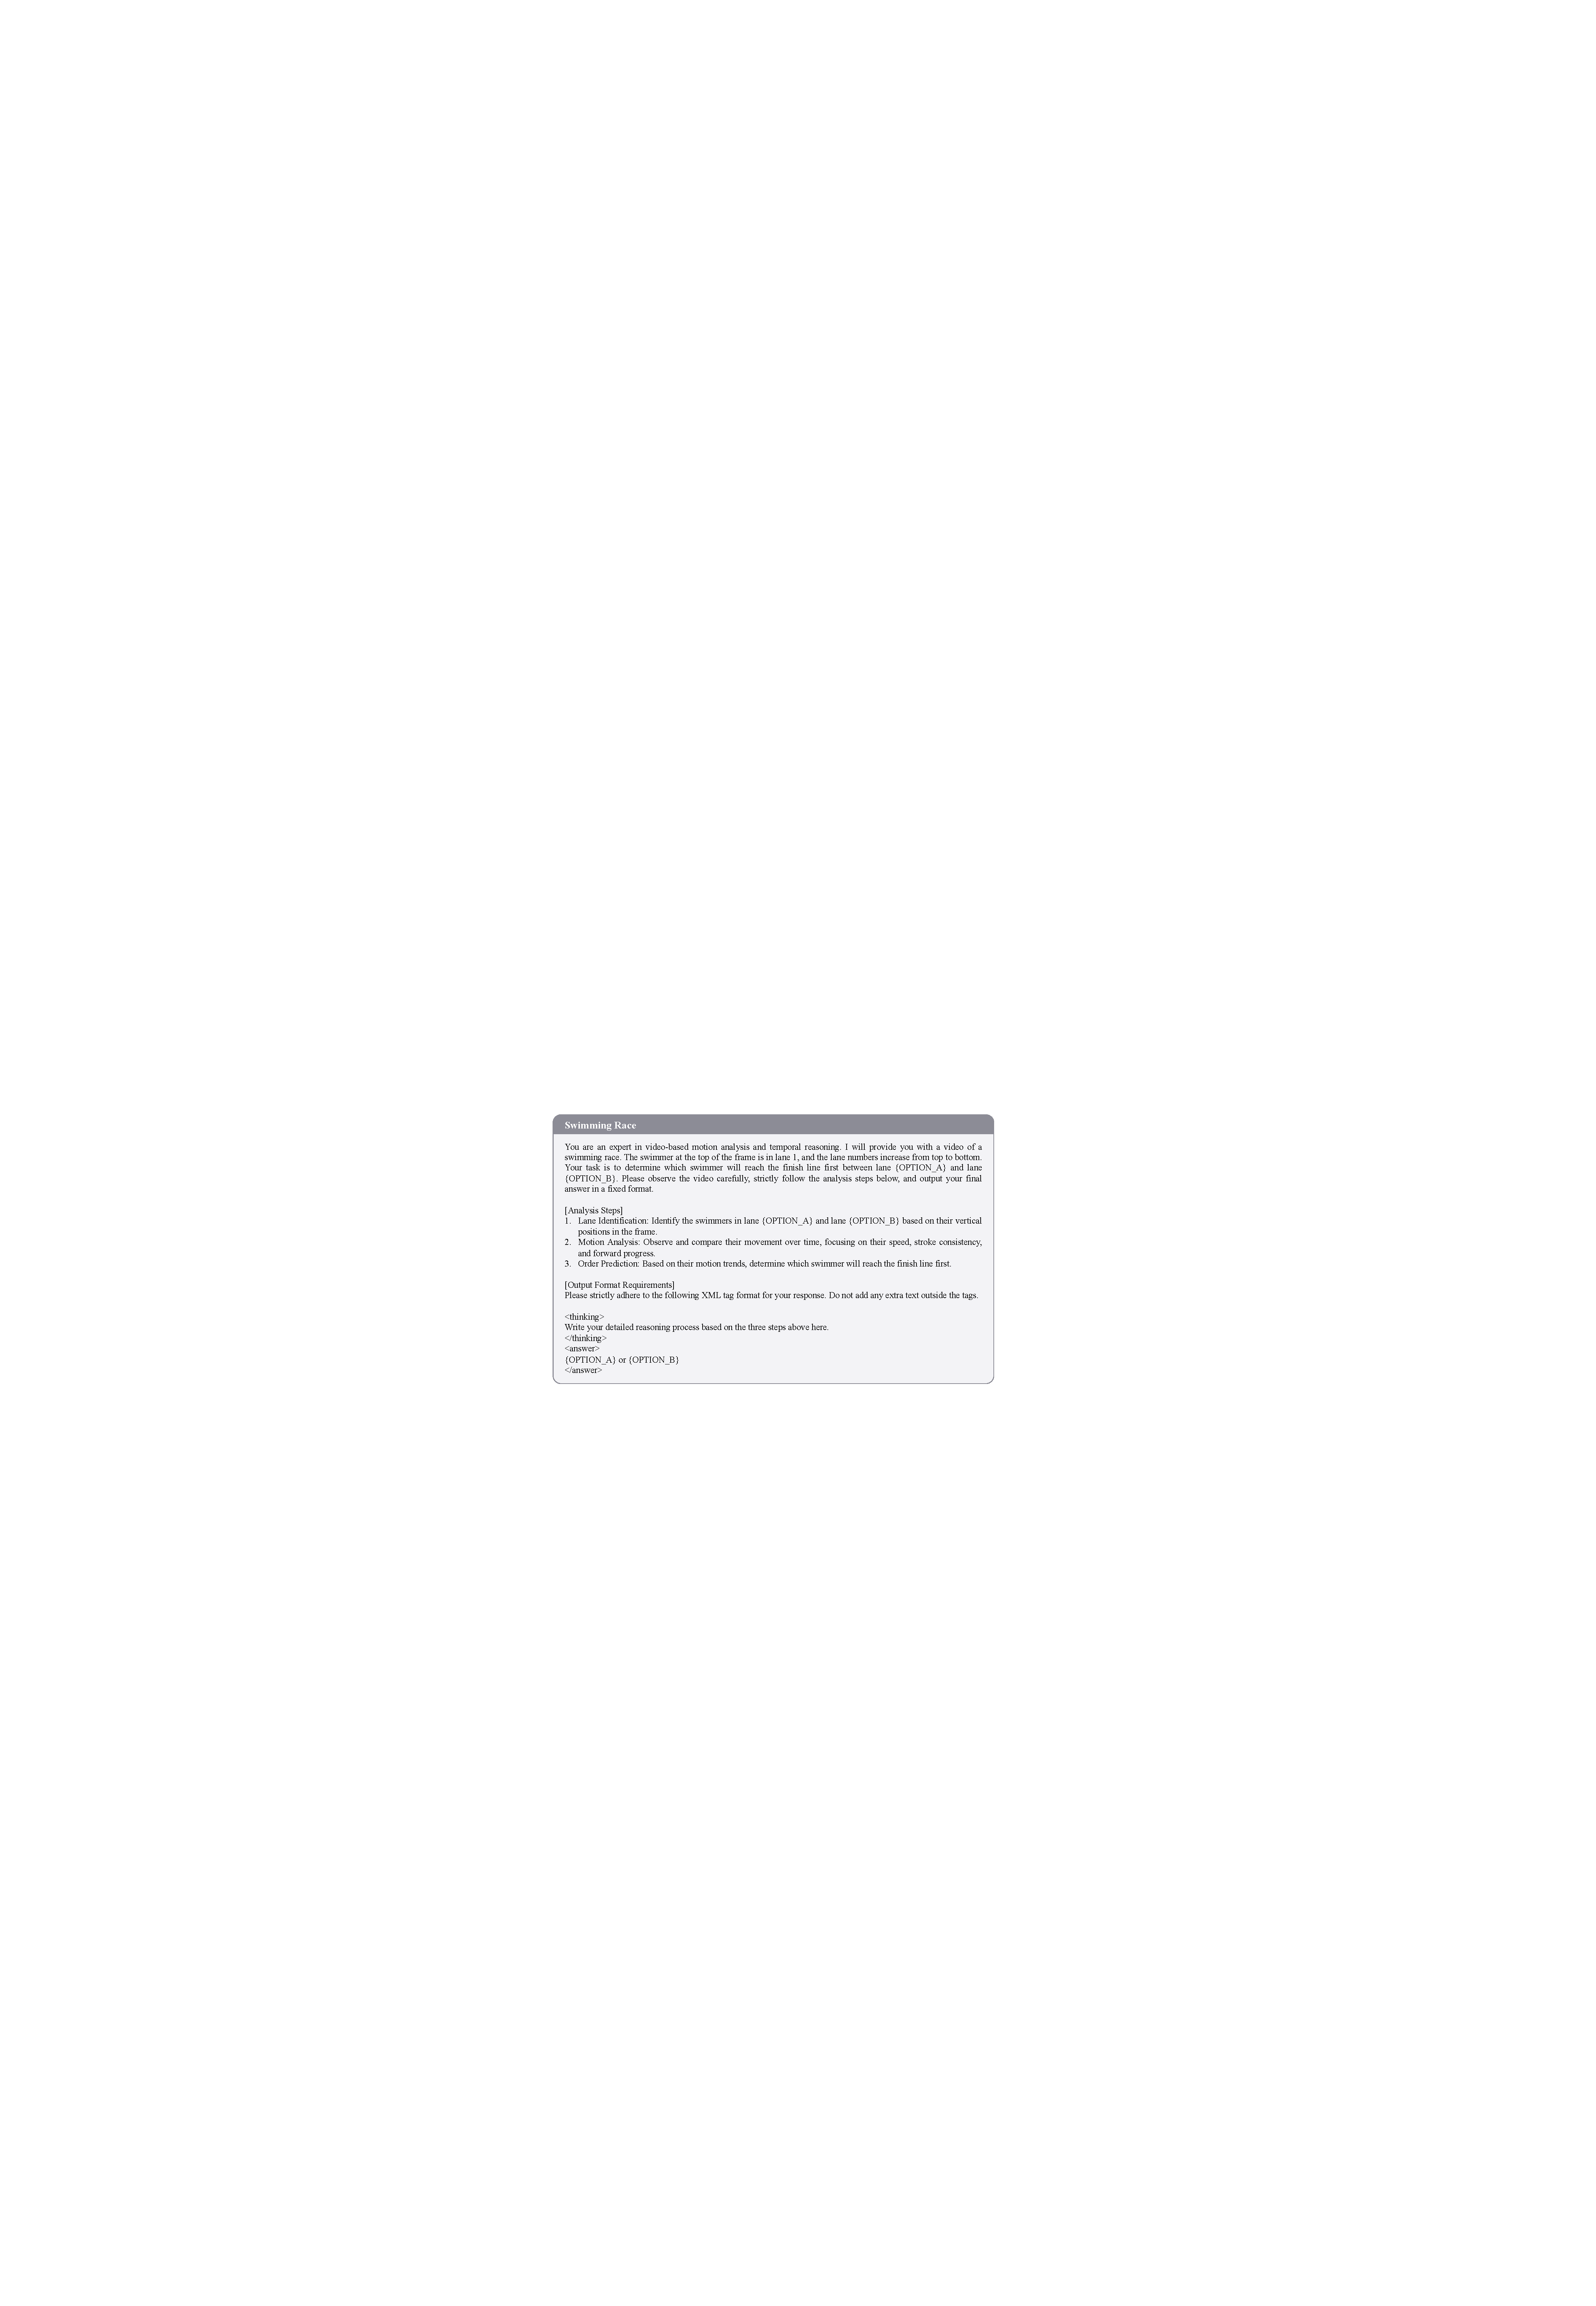
\includegraphics[width=0.95\linewidth]{fig/fig_14.pdf}
  \caption{\textbf{Manual CoT prompt template for Swimming Race.}}
  \label{fig:14}
\end{figure}

\begin{figure}[p]
  \centering
  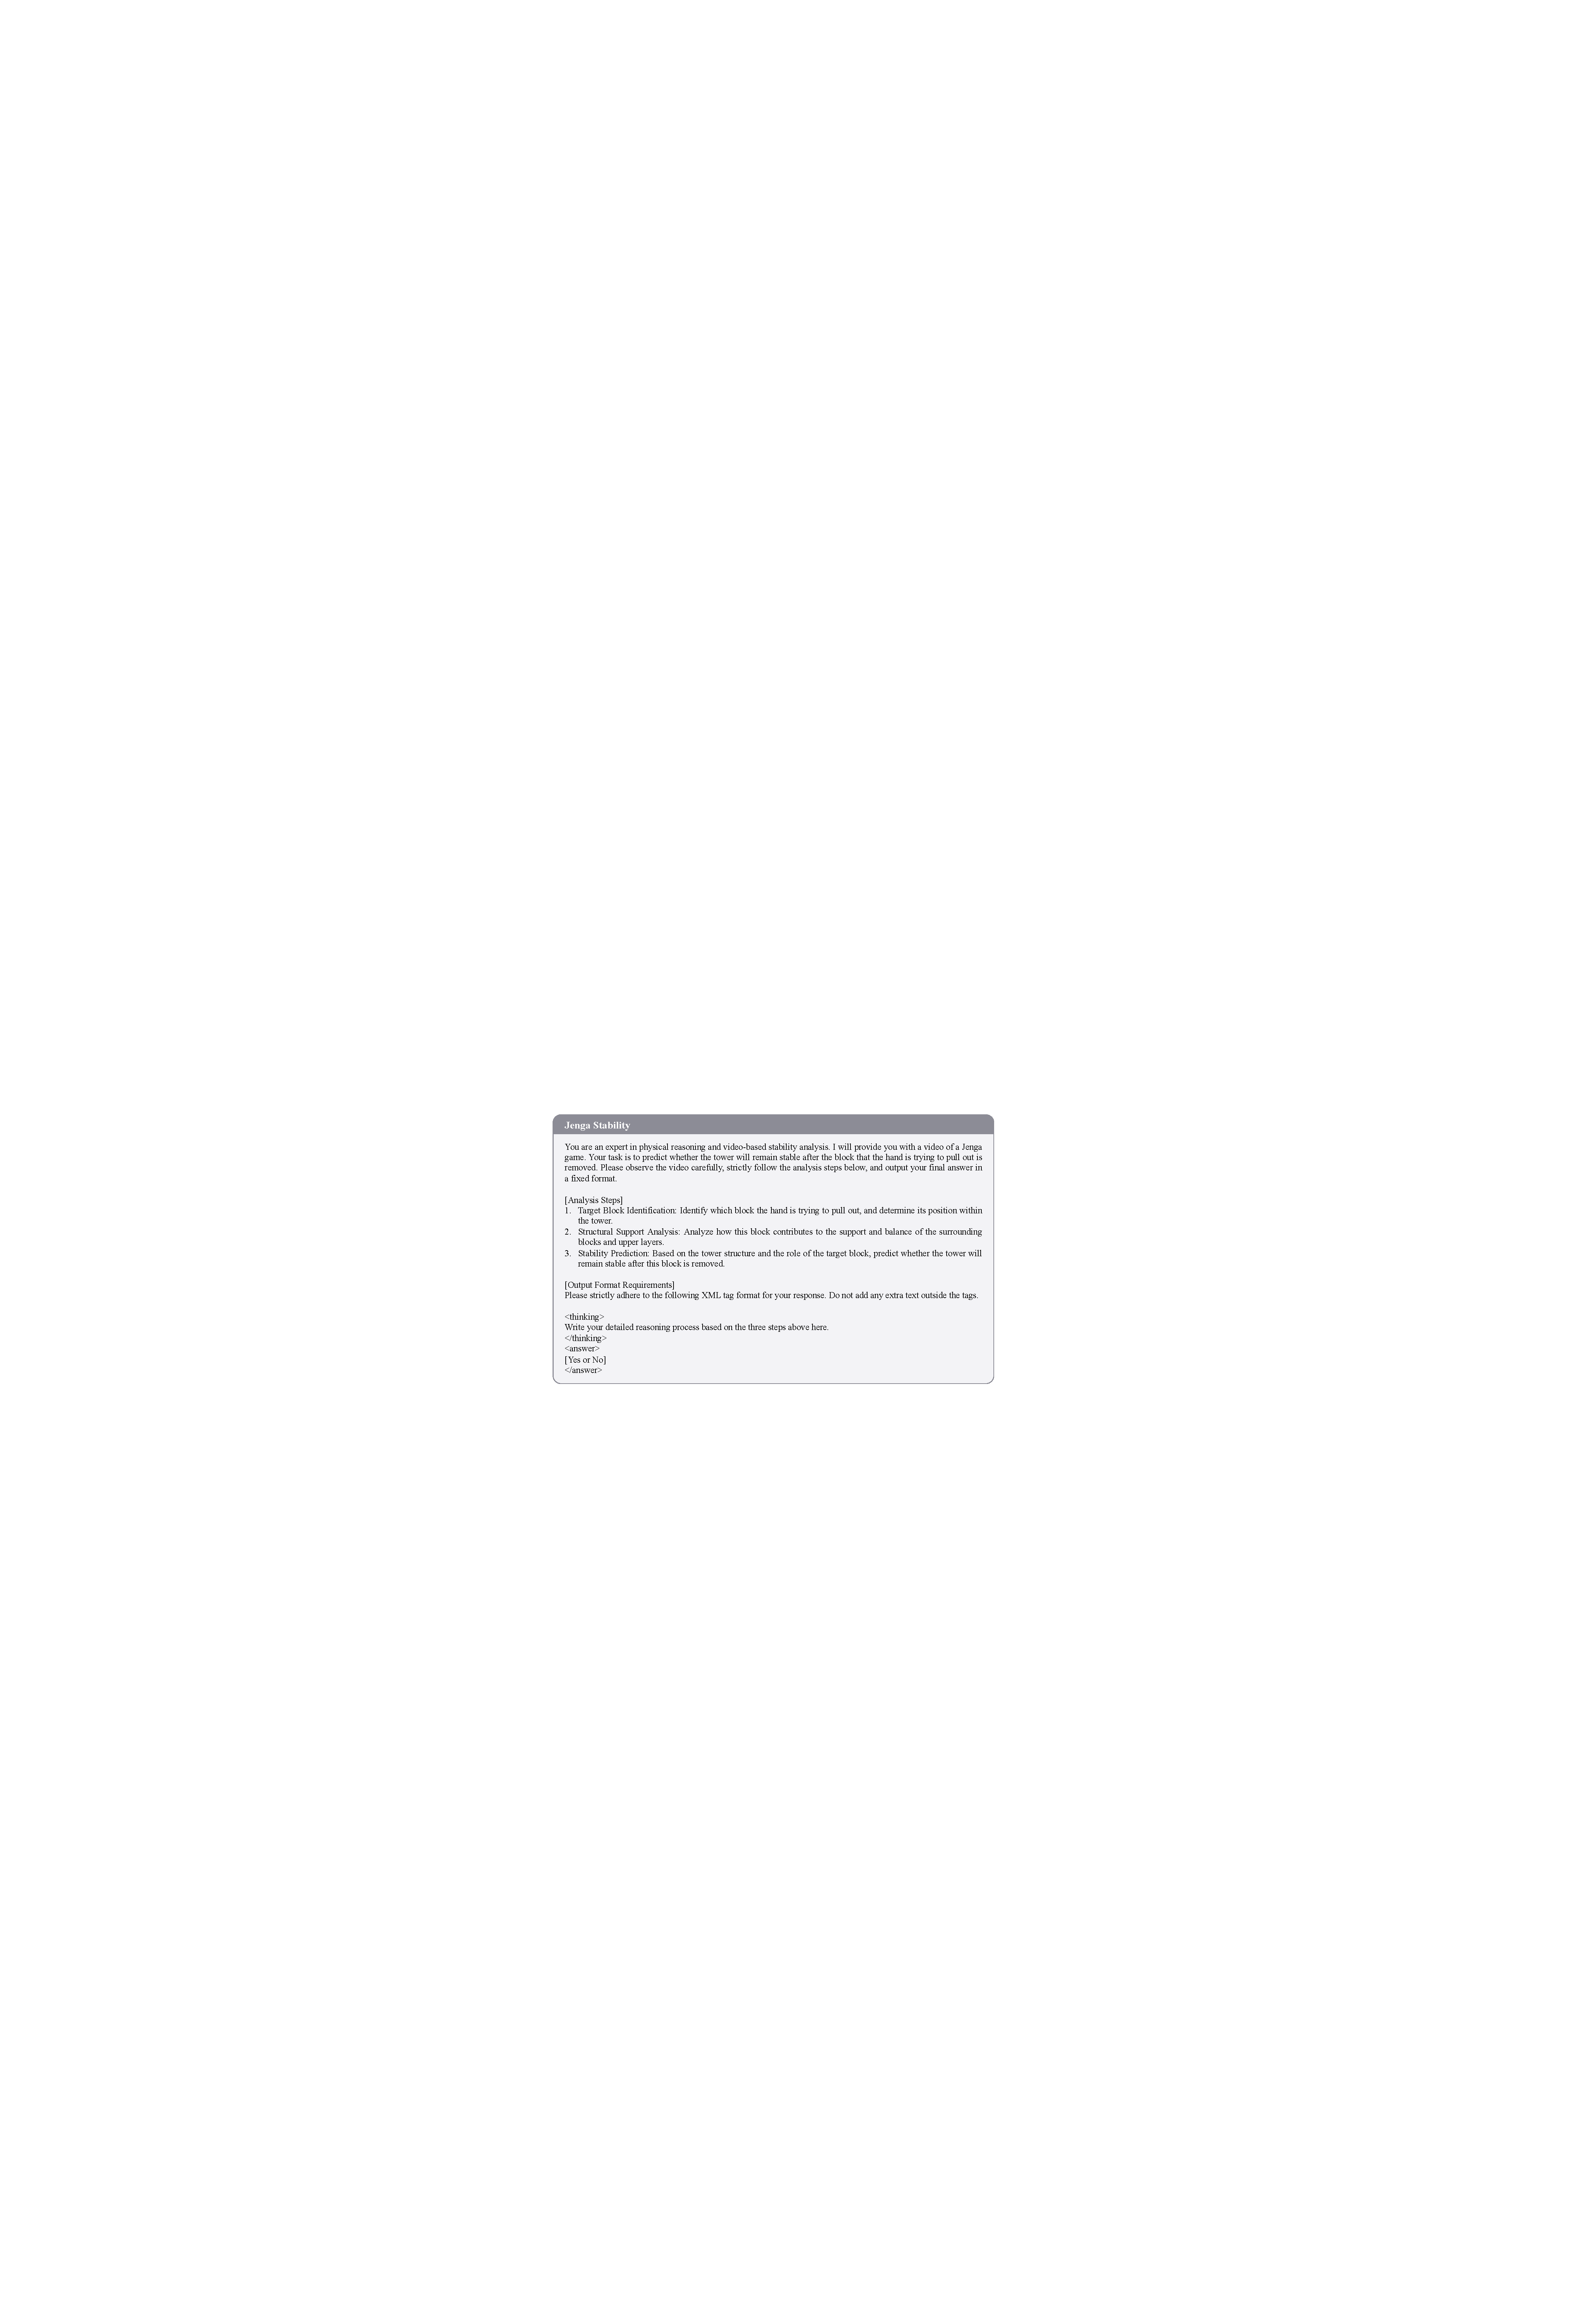
\includegraphics[width=0.95\linewidth]{fig/fig_15.pdf}
  \caption{\textbf{Manual CoT prompt template for Jenga Stability.}}
  \label{fig:15}
\end{figure}

\begin{figure}[p]
  \centering
  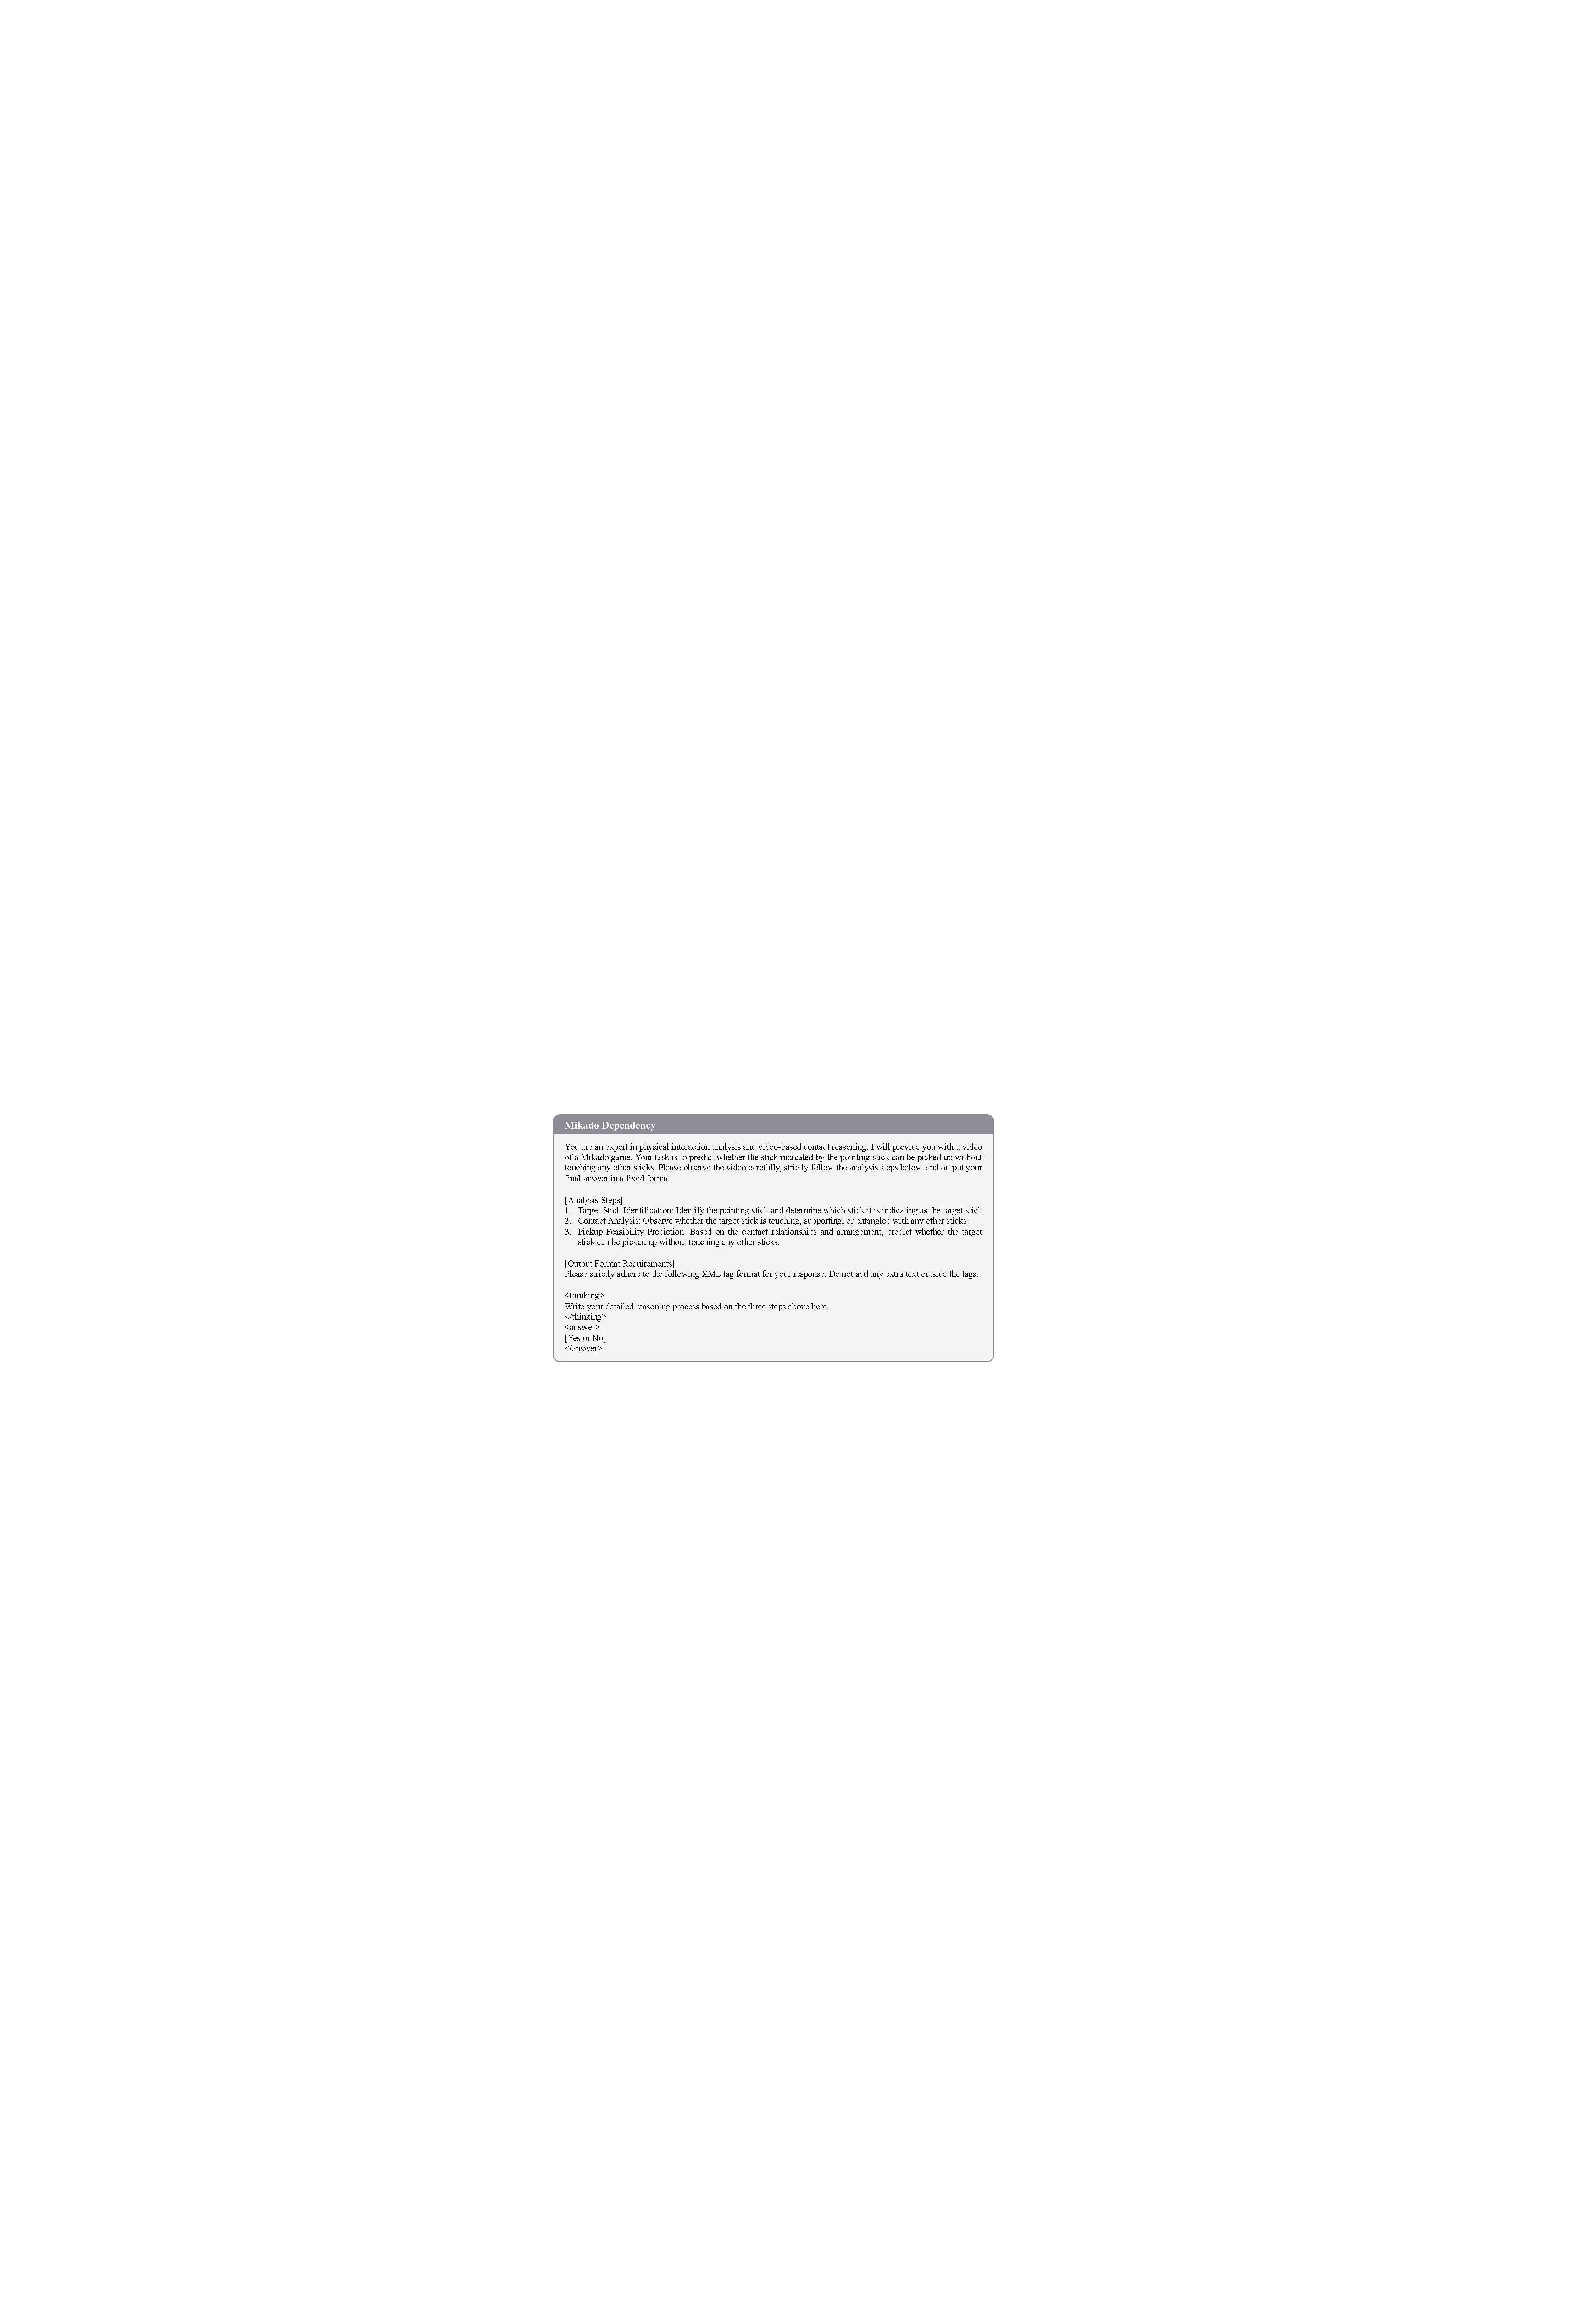
\includegraphics[width=0.95\linewidth]{fig/fig_16.pdf}
  \caption{\textbf{Manual CoT prompt template for Mikado Dependency.}}
  \label{fig:16}
\end{figure}

\begin{figure}[p]
  \centering
  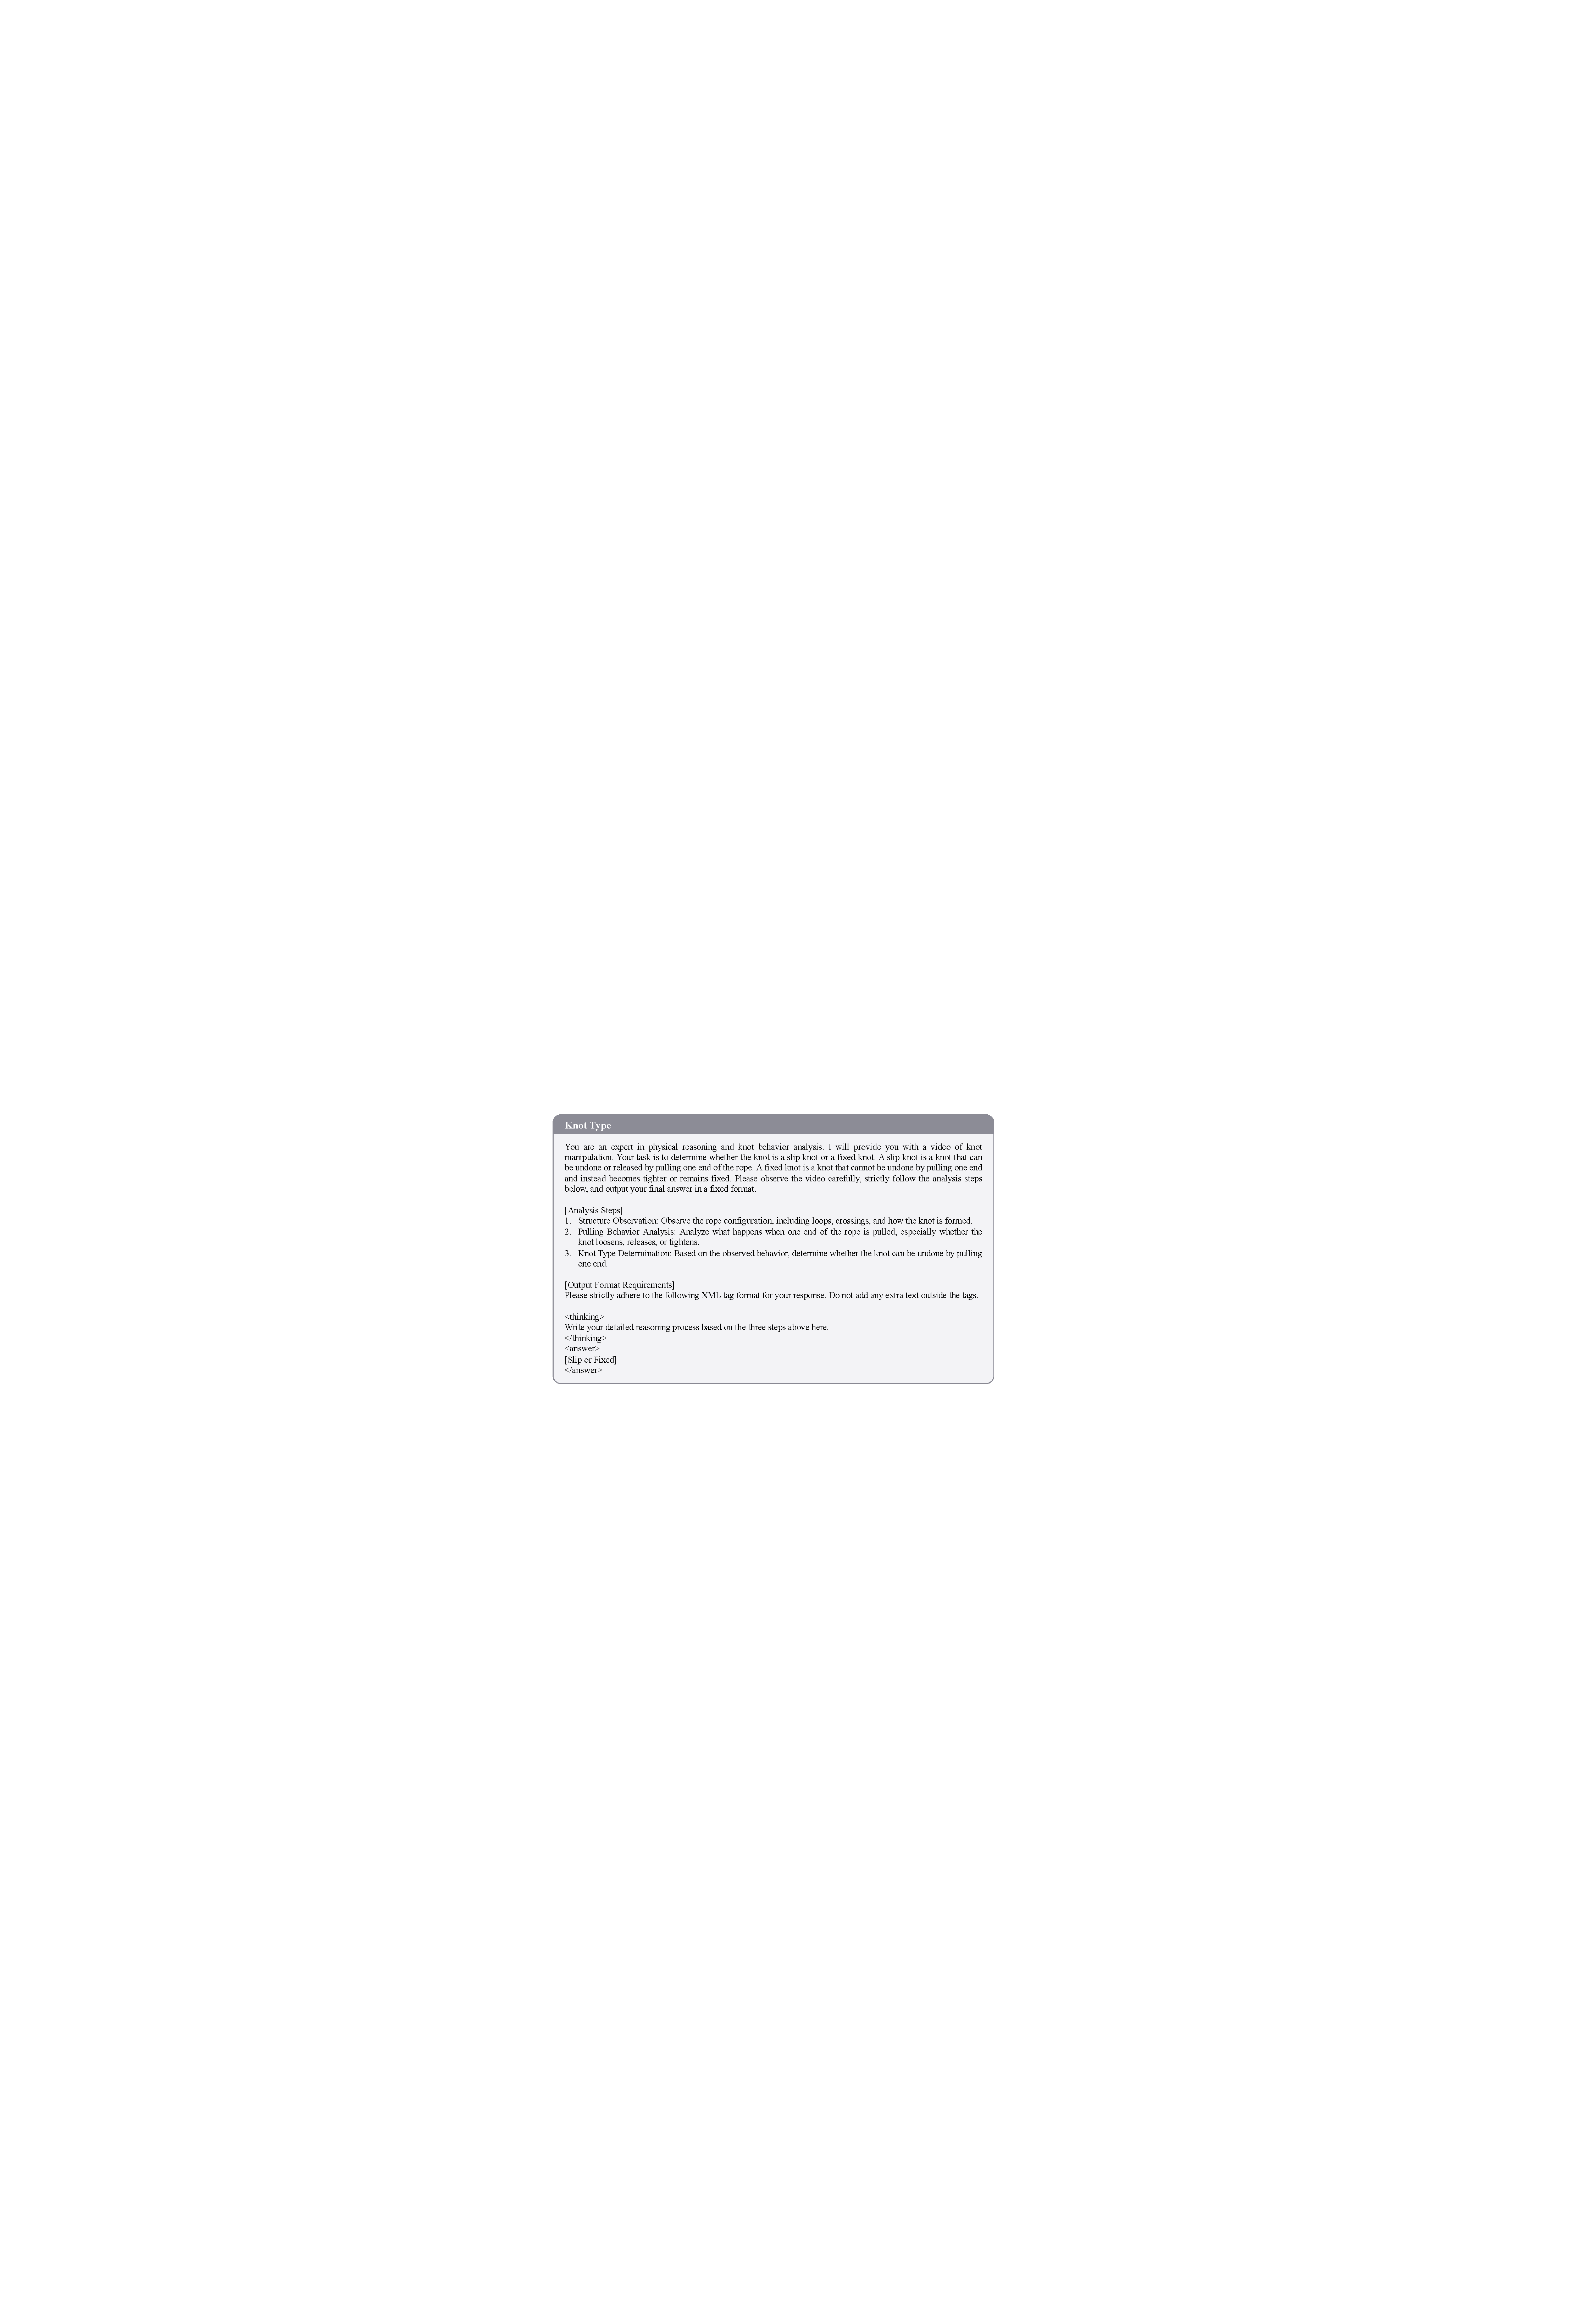
\includegraphics[width=0.95\linewidth]{fig/fig_17.pdf}
  \caption{\textbf{Manual CoT prompt template for Knot Type.}}
  \label{fig:17}
\end{figure}

\begin{figure}[p]
  \centering
  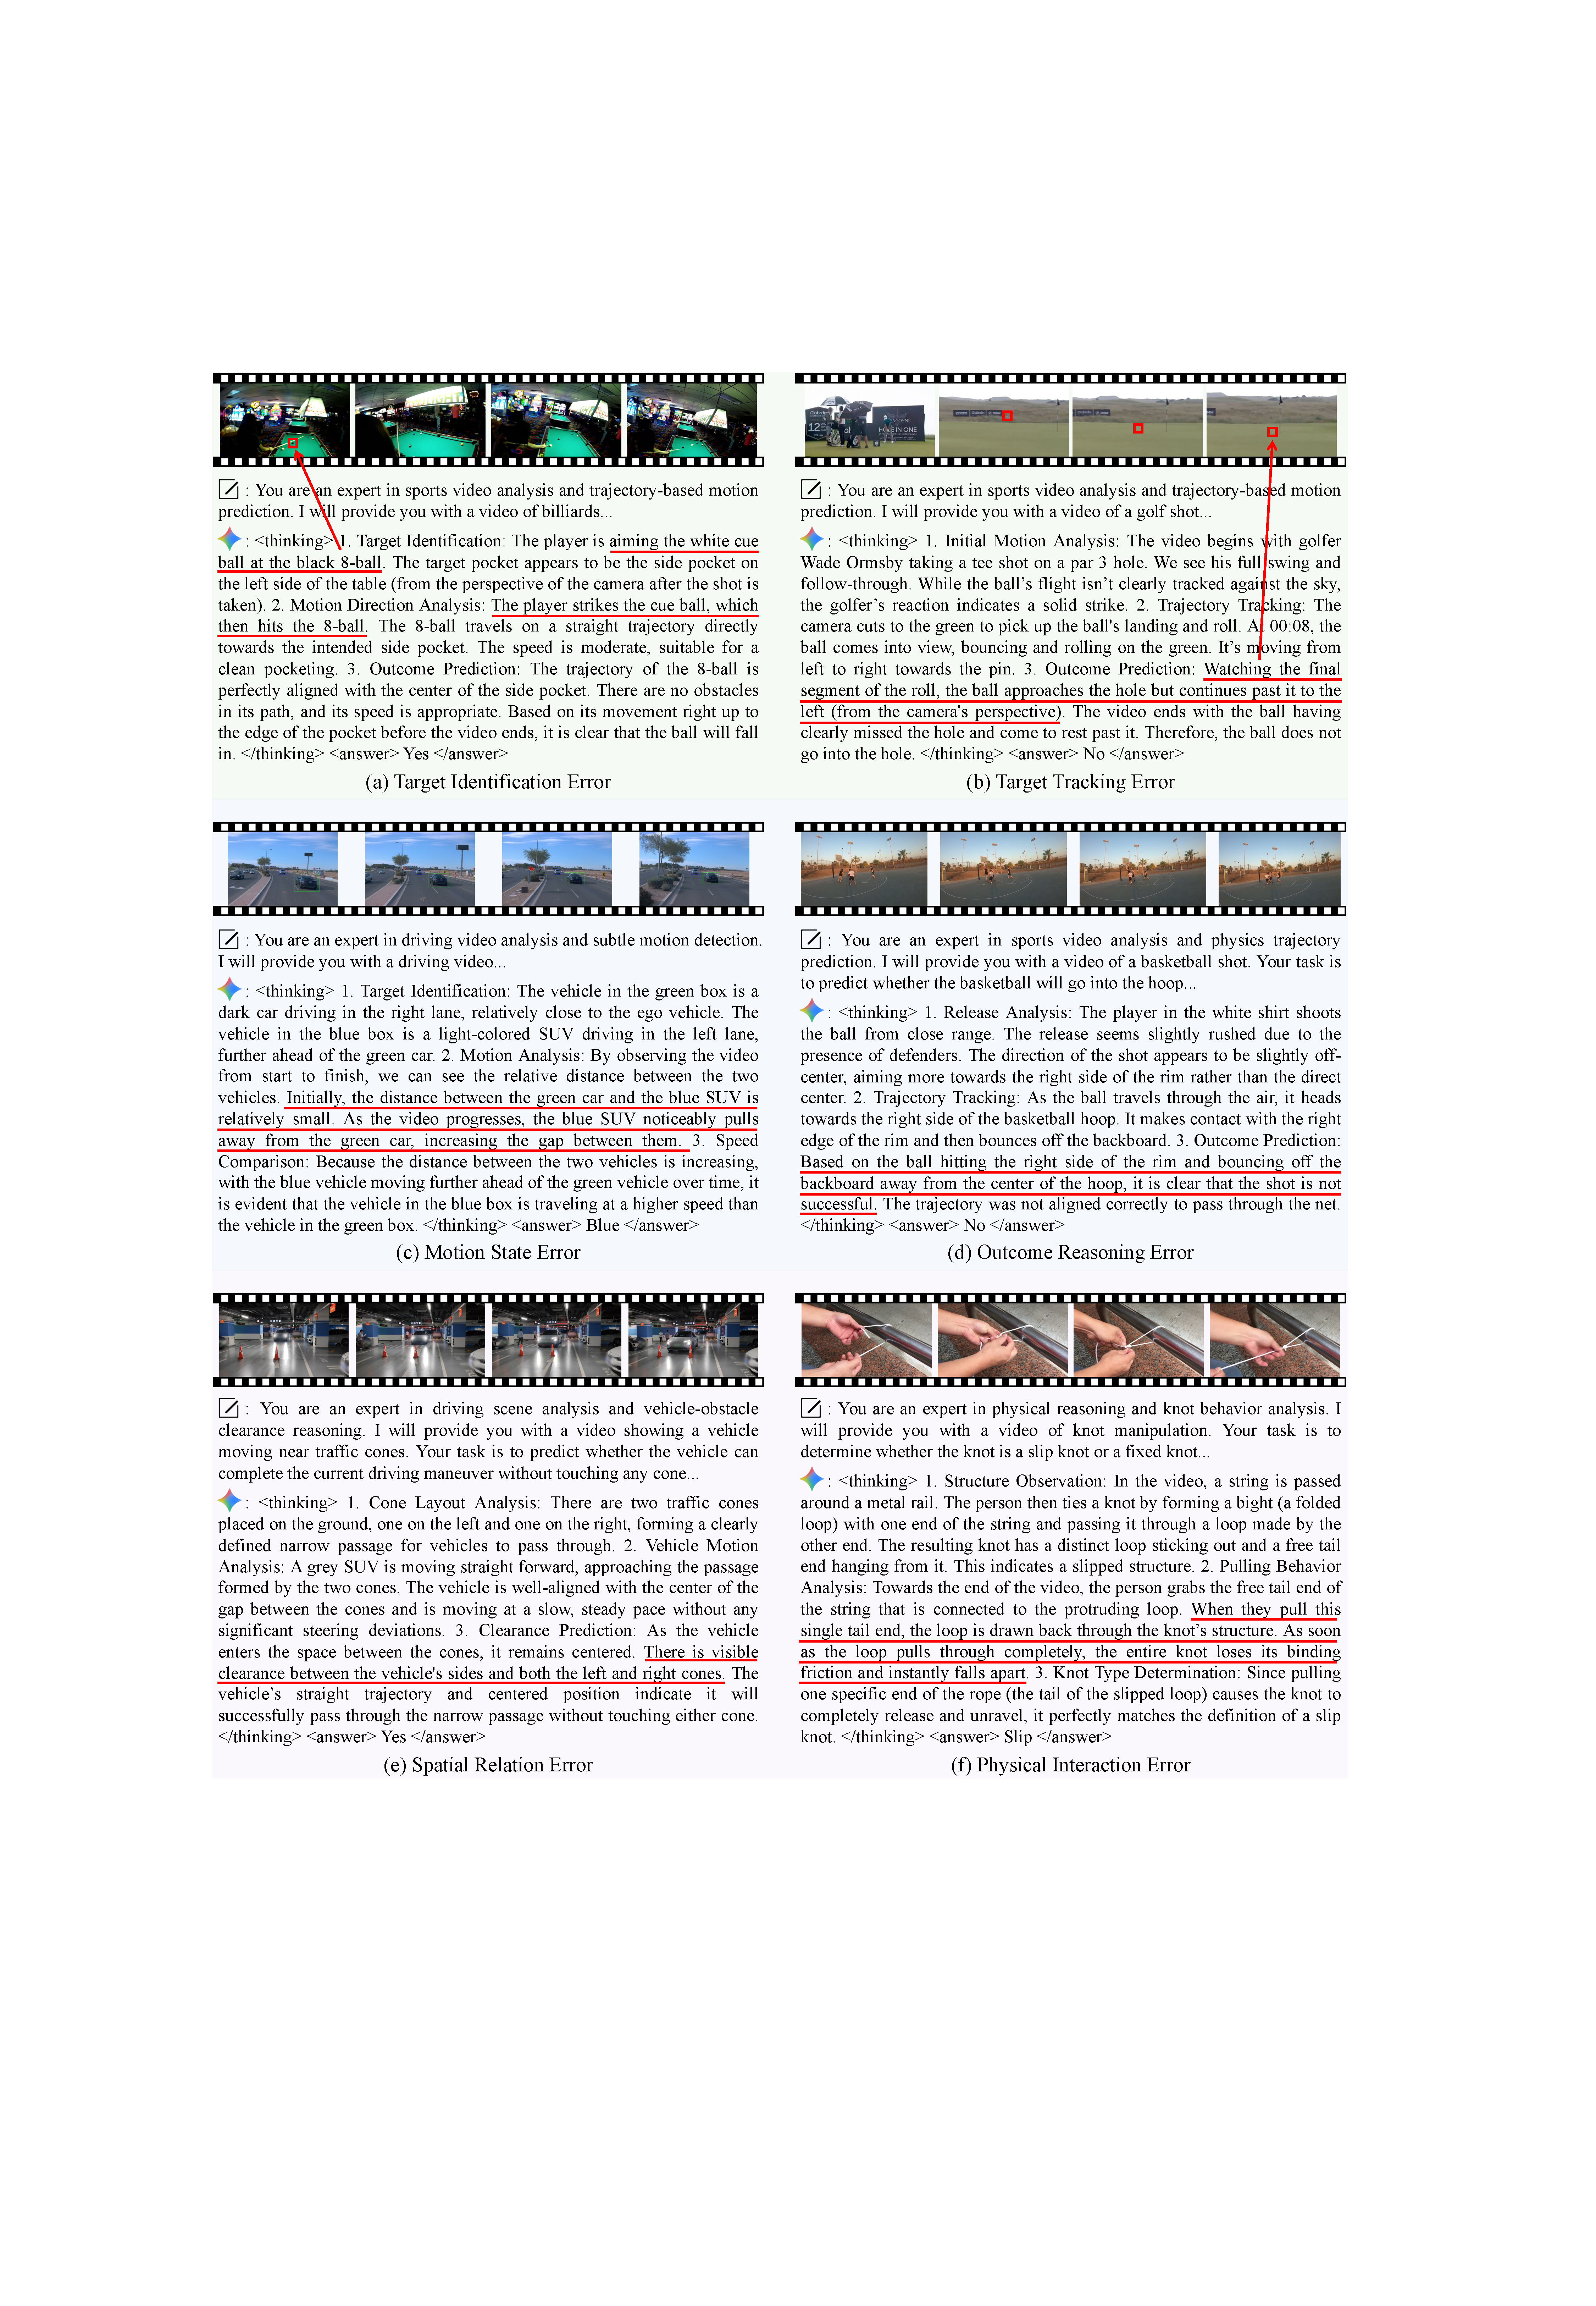
\includegraphics[width=0.95\linewidth]{fig/fig_18.pdf}
  \caption{\textbf{Representative examples for each primary error type.}}
  \label{fig:18}
\end{figure}

\begin{figure}[p]
  \centering
  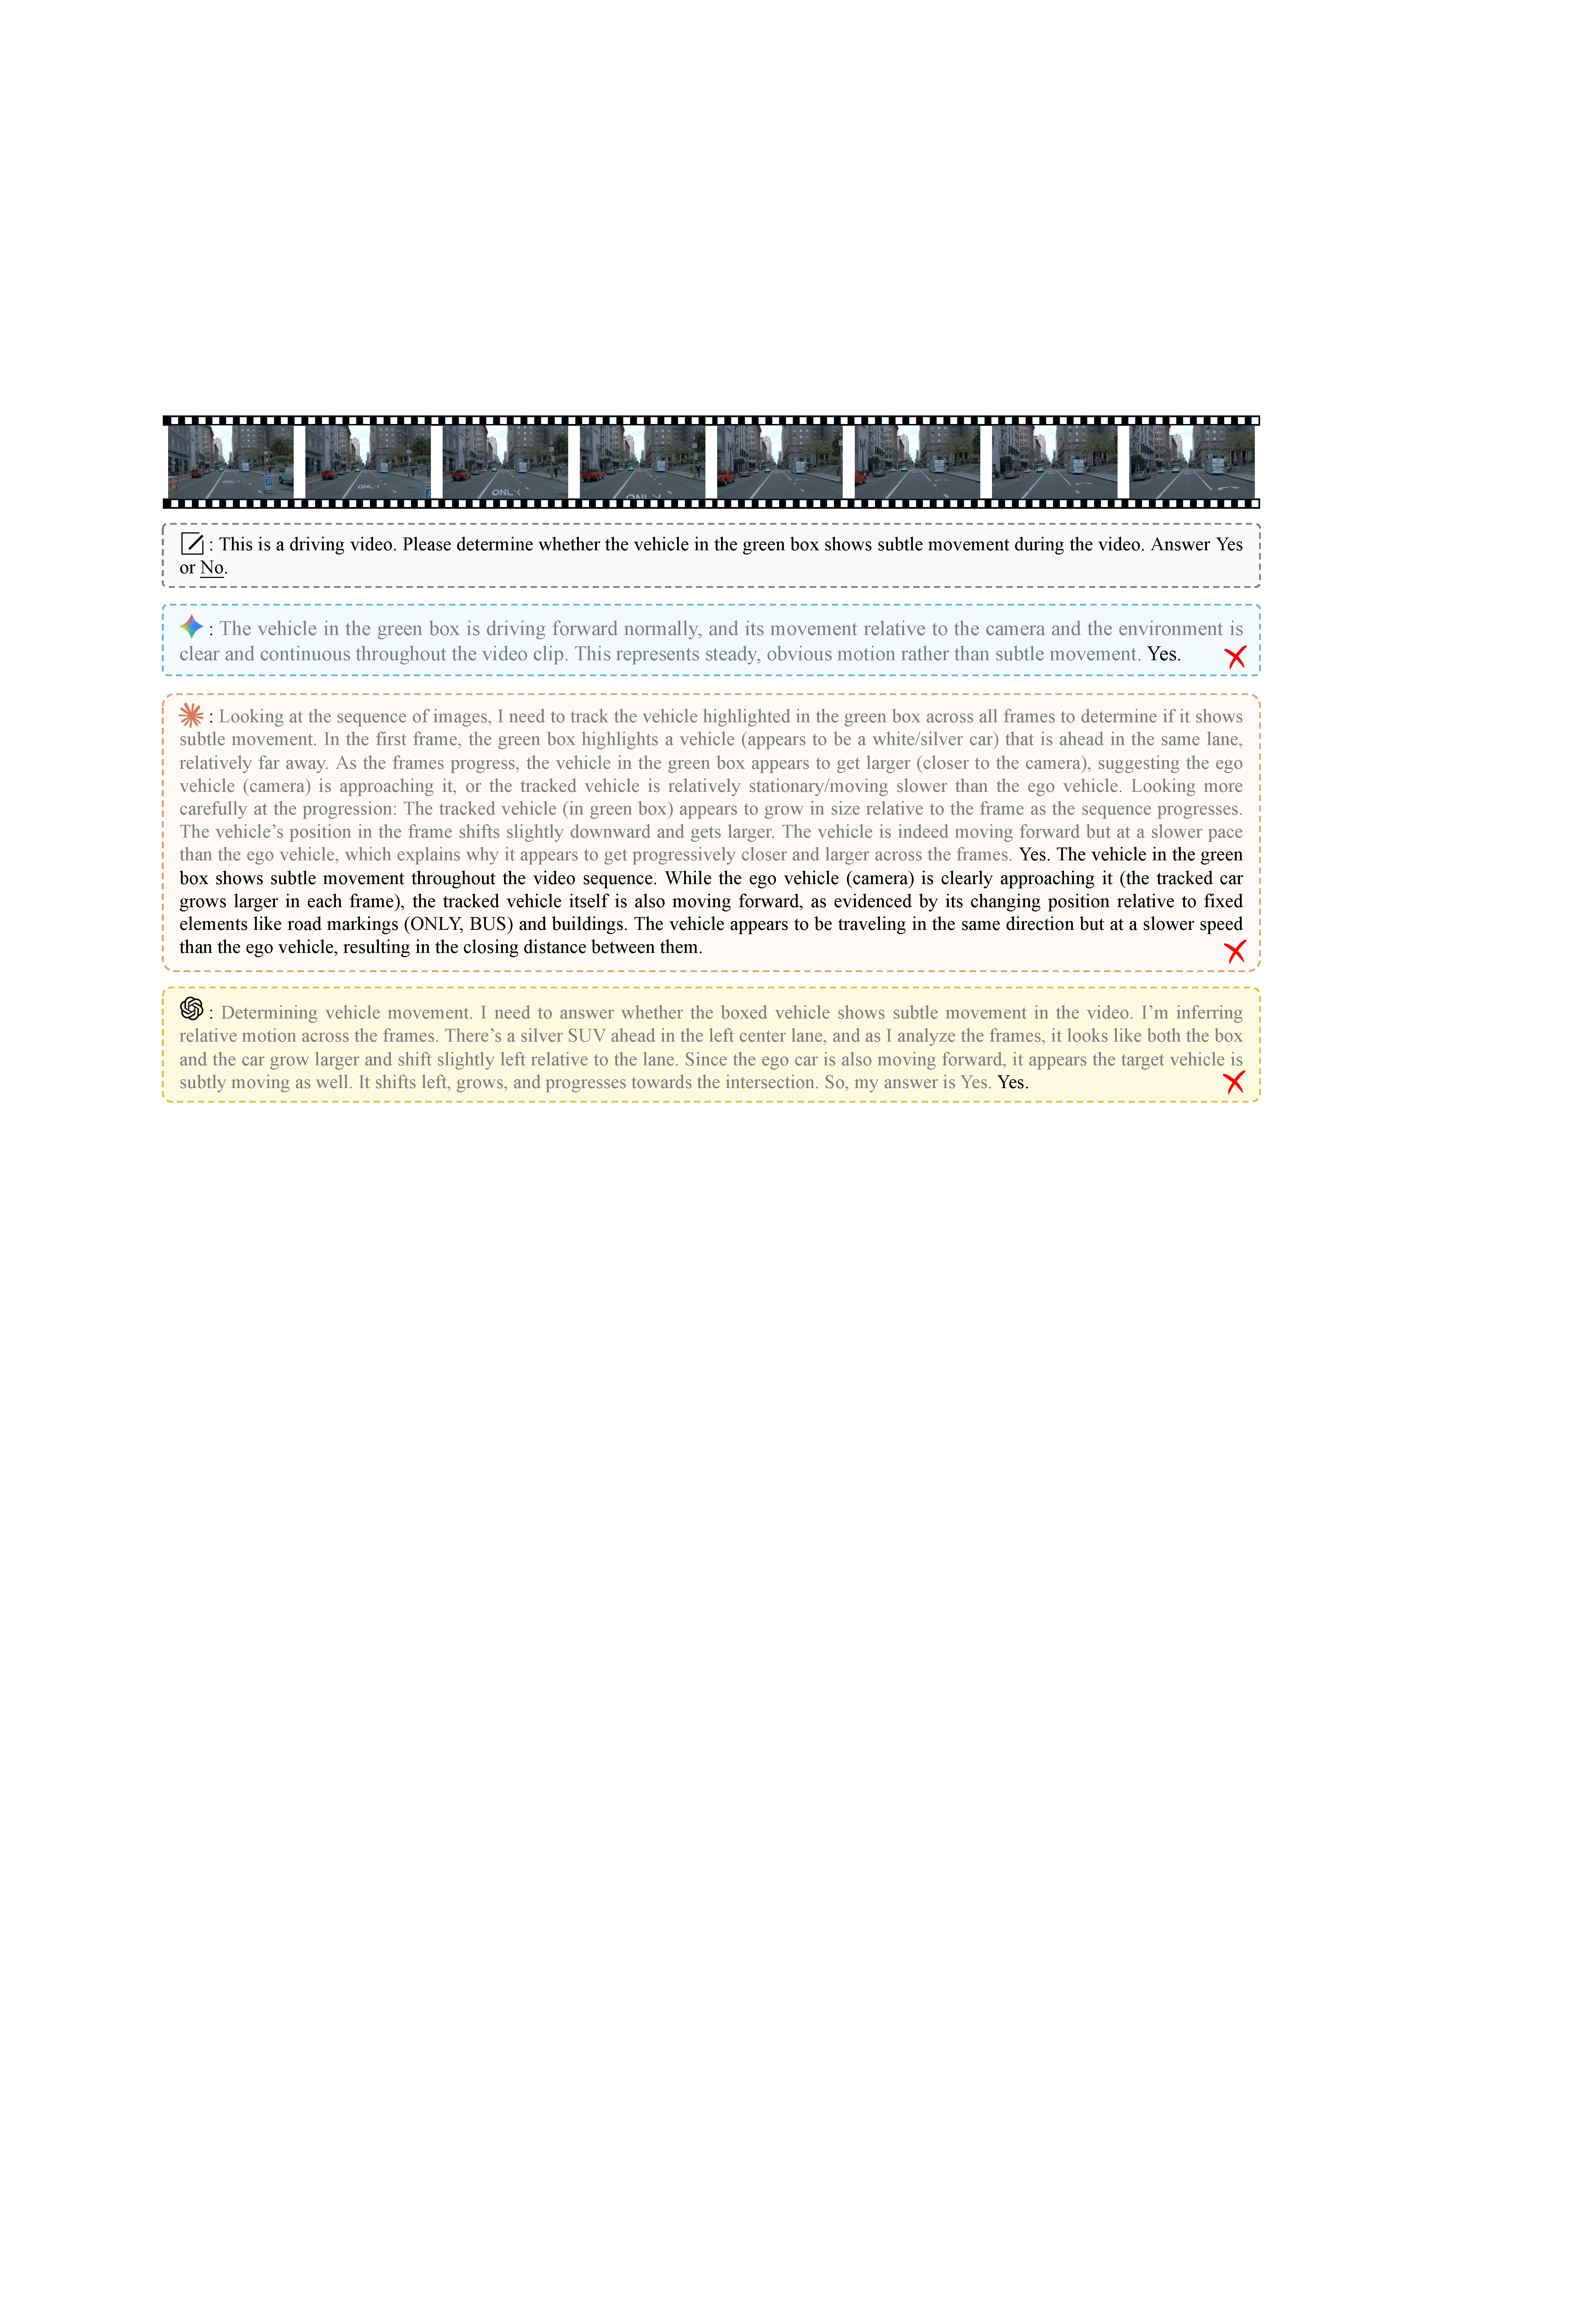
\includegraphics[width=0.95\linewidth]{fig/fig_19.pdf}
  \caption{\textbf{Qualitative visualization for Vehicle Movement.}
  We compare the outputs of GPT-5.4-thinking~\citep{GPT-5}, Gemini-3.1-Pro-Preview~\citep{Gemini}, and Claude-Opus-4.6-thinking~\citep{Claude}.
  Gray text denotes built-in thinking content.}
  \label{fig:19}
\end{figure}

\begin{figure}[p]
  \centering
  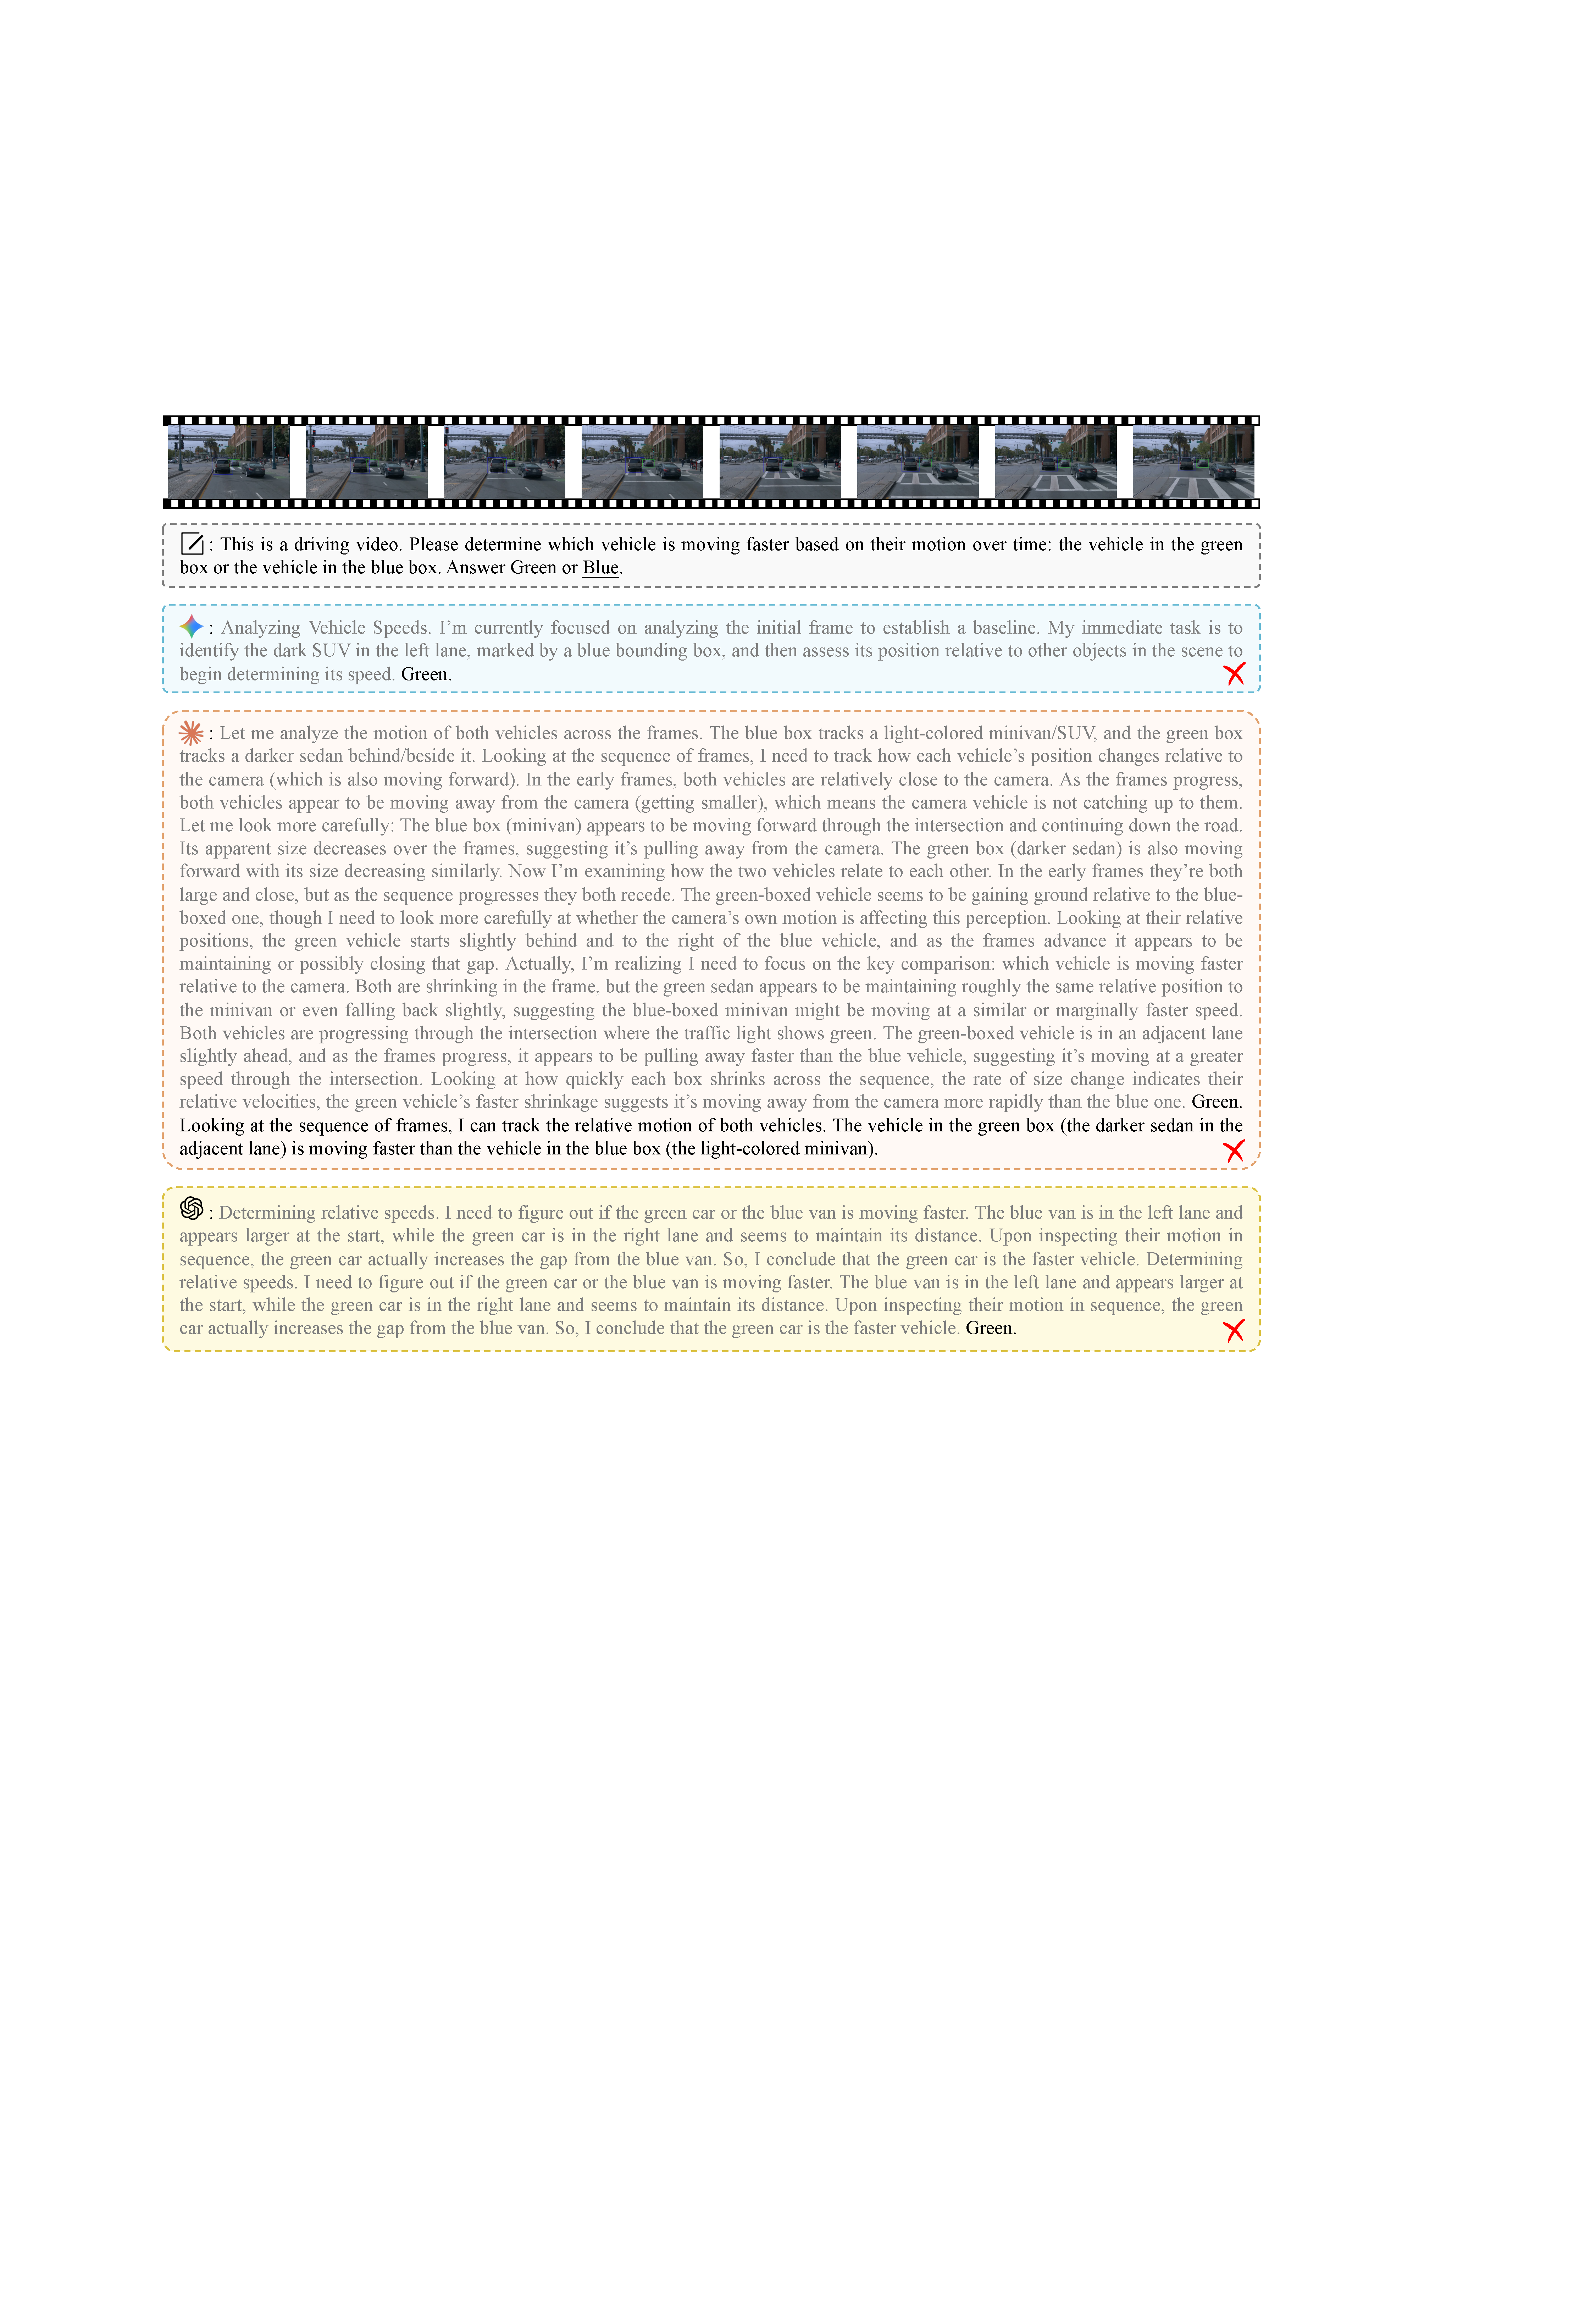
\includegraphics[width=0.95\linewidth]{fig/fig_20.pdf}
  \caption{\textbf{Qualitative visualization for Relative Velocity.}
  We compare the outputs of GPT-5.4-thinking~\citep{GPT-5}, Gemini-3.1-Pro-Preview~\citep{Gemini}, and Claude-Opus-4.6-thinking~\citep{Claude}.
  Gray text denotes built-in thinking content.}
  \label{fig:20}
\end{figure}

\begin{figure}[p]
  \centering
  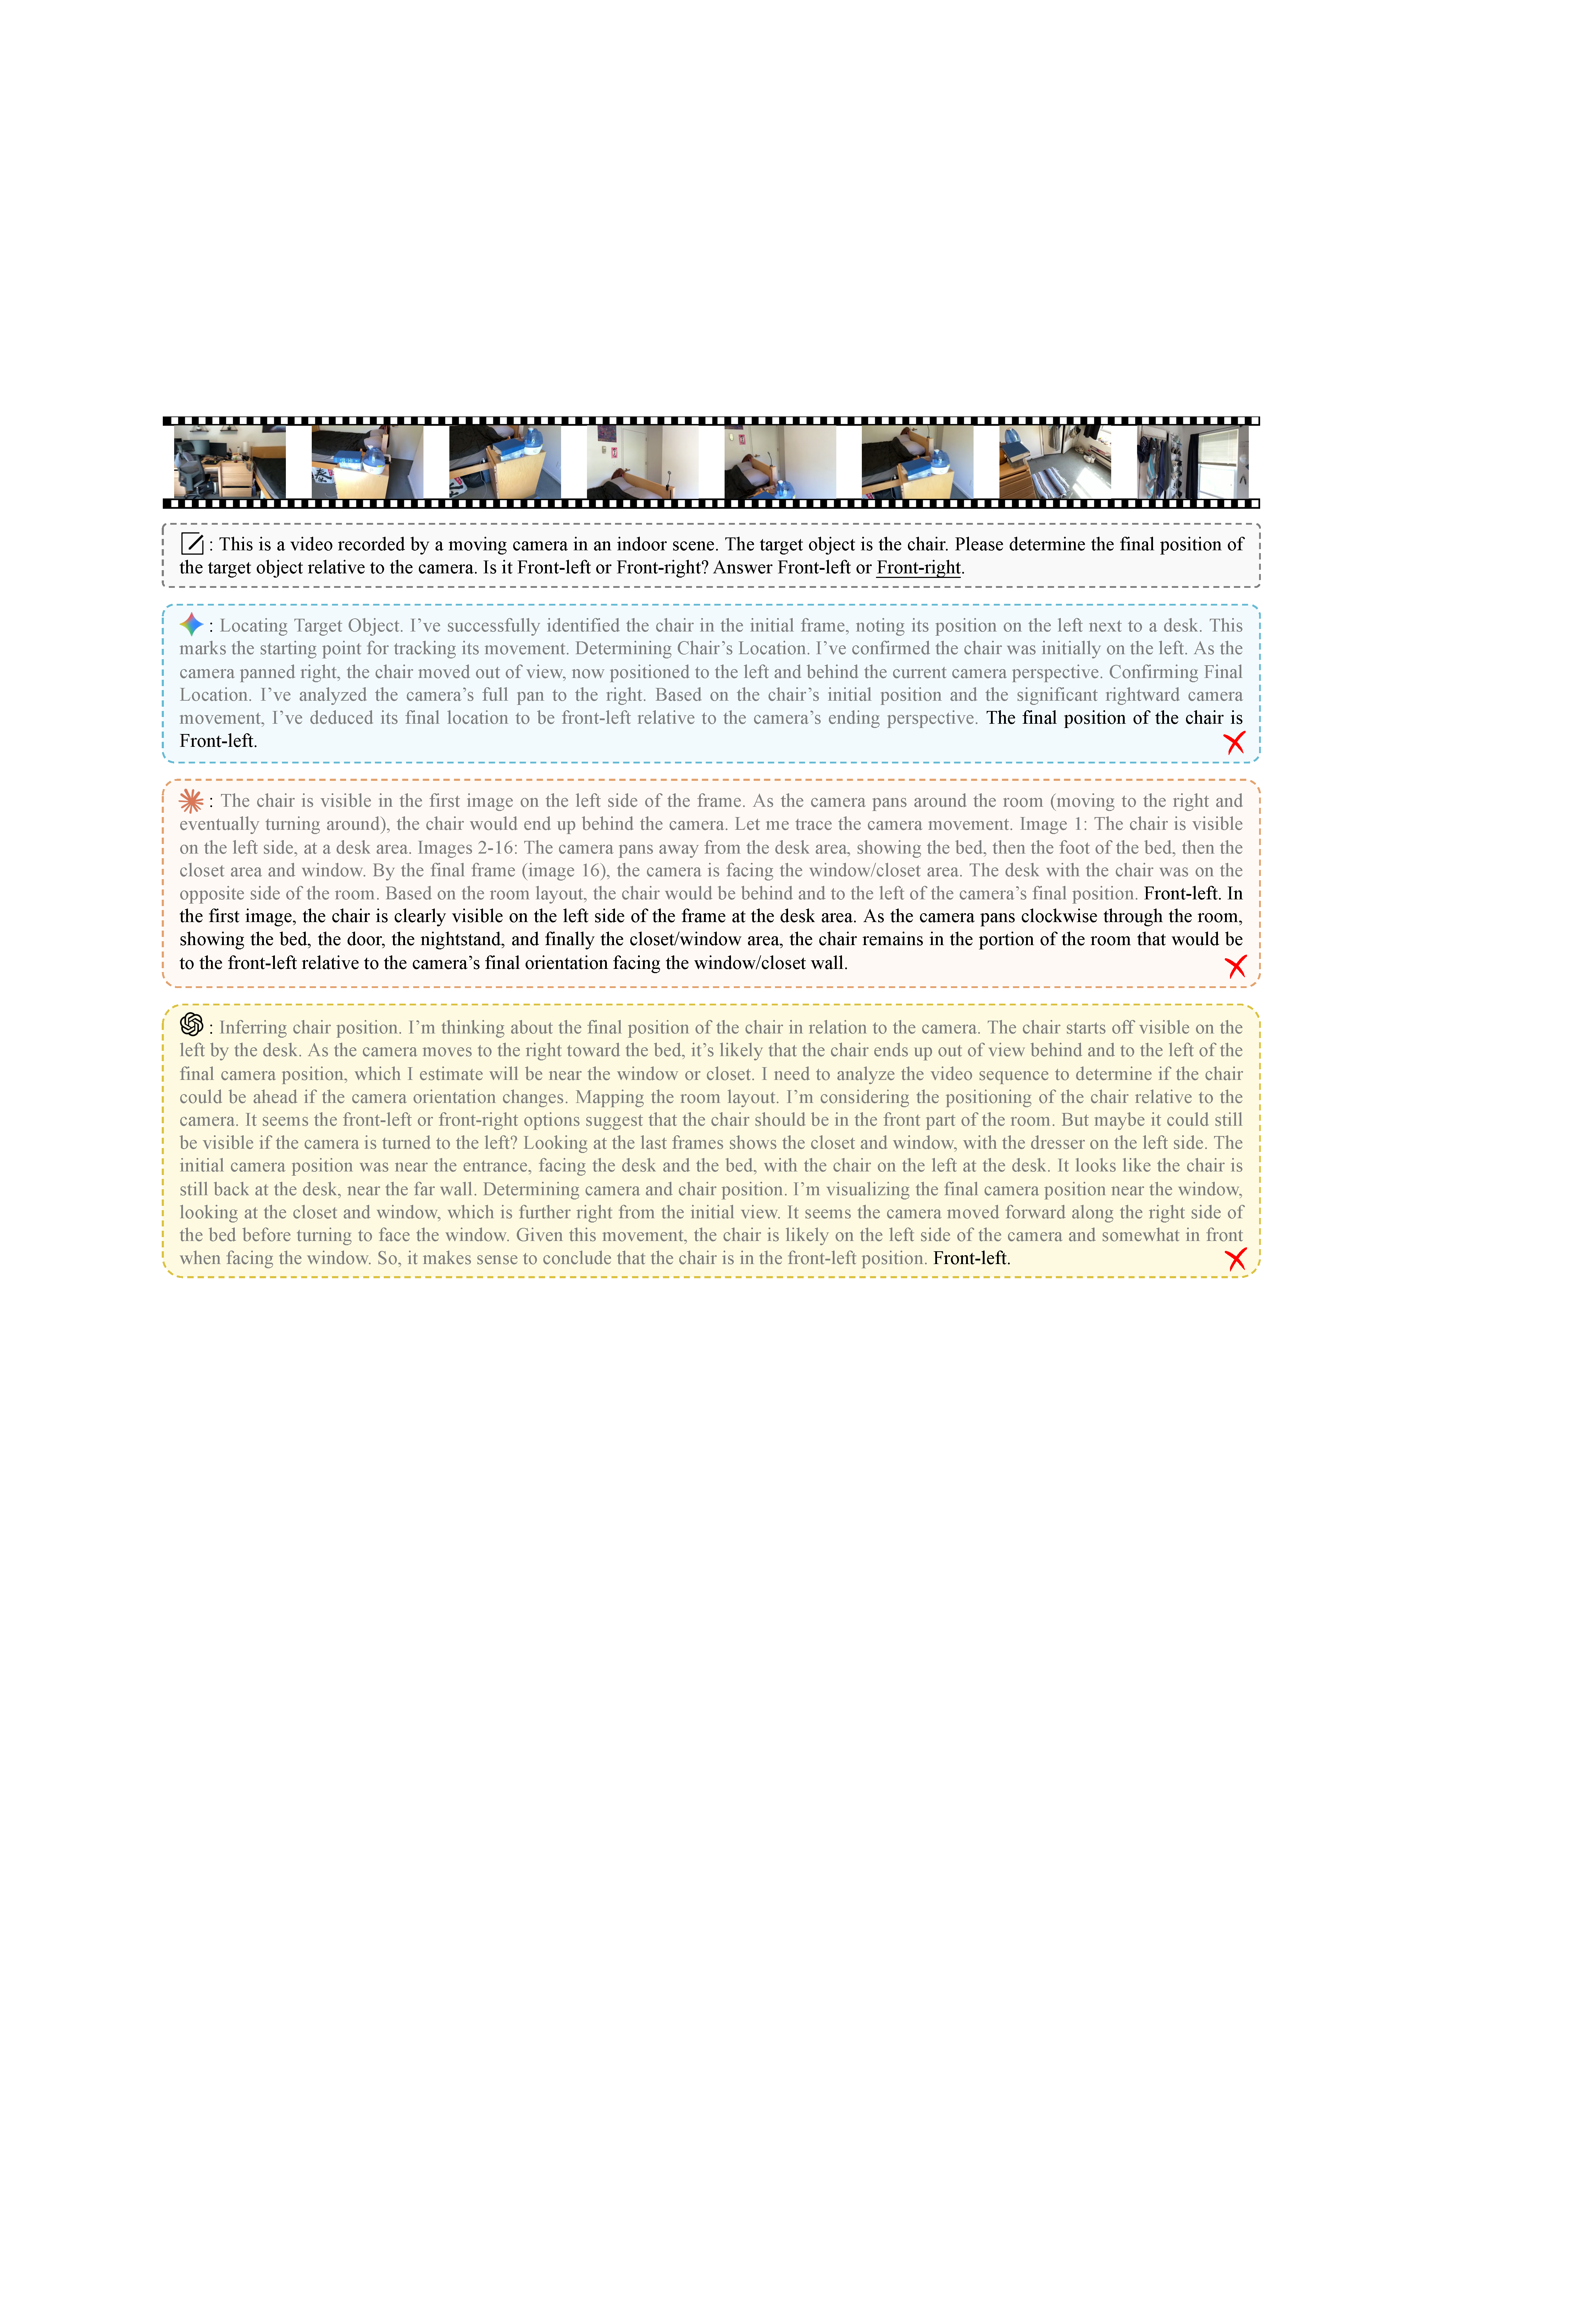
\includegraphics[width=0.95\linewidth]{fig/fig_21.pdf}
  \caption{\textbf{Qualitative visualization for Ego Motion.}
  We compare the outputs of GPT-5.4-thinking~\citep{GPT-5}, Gemini-3.1-Pro-Preview~\citep{Gemini}, and Claude-Opus-4.6-thinking~\citep{Claude}.
  Gray text denotes built-in thinking content.}
  \label{fig:21}
\end{figure}

\begin{figure}[p]
  \centering
  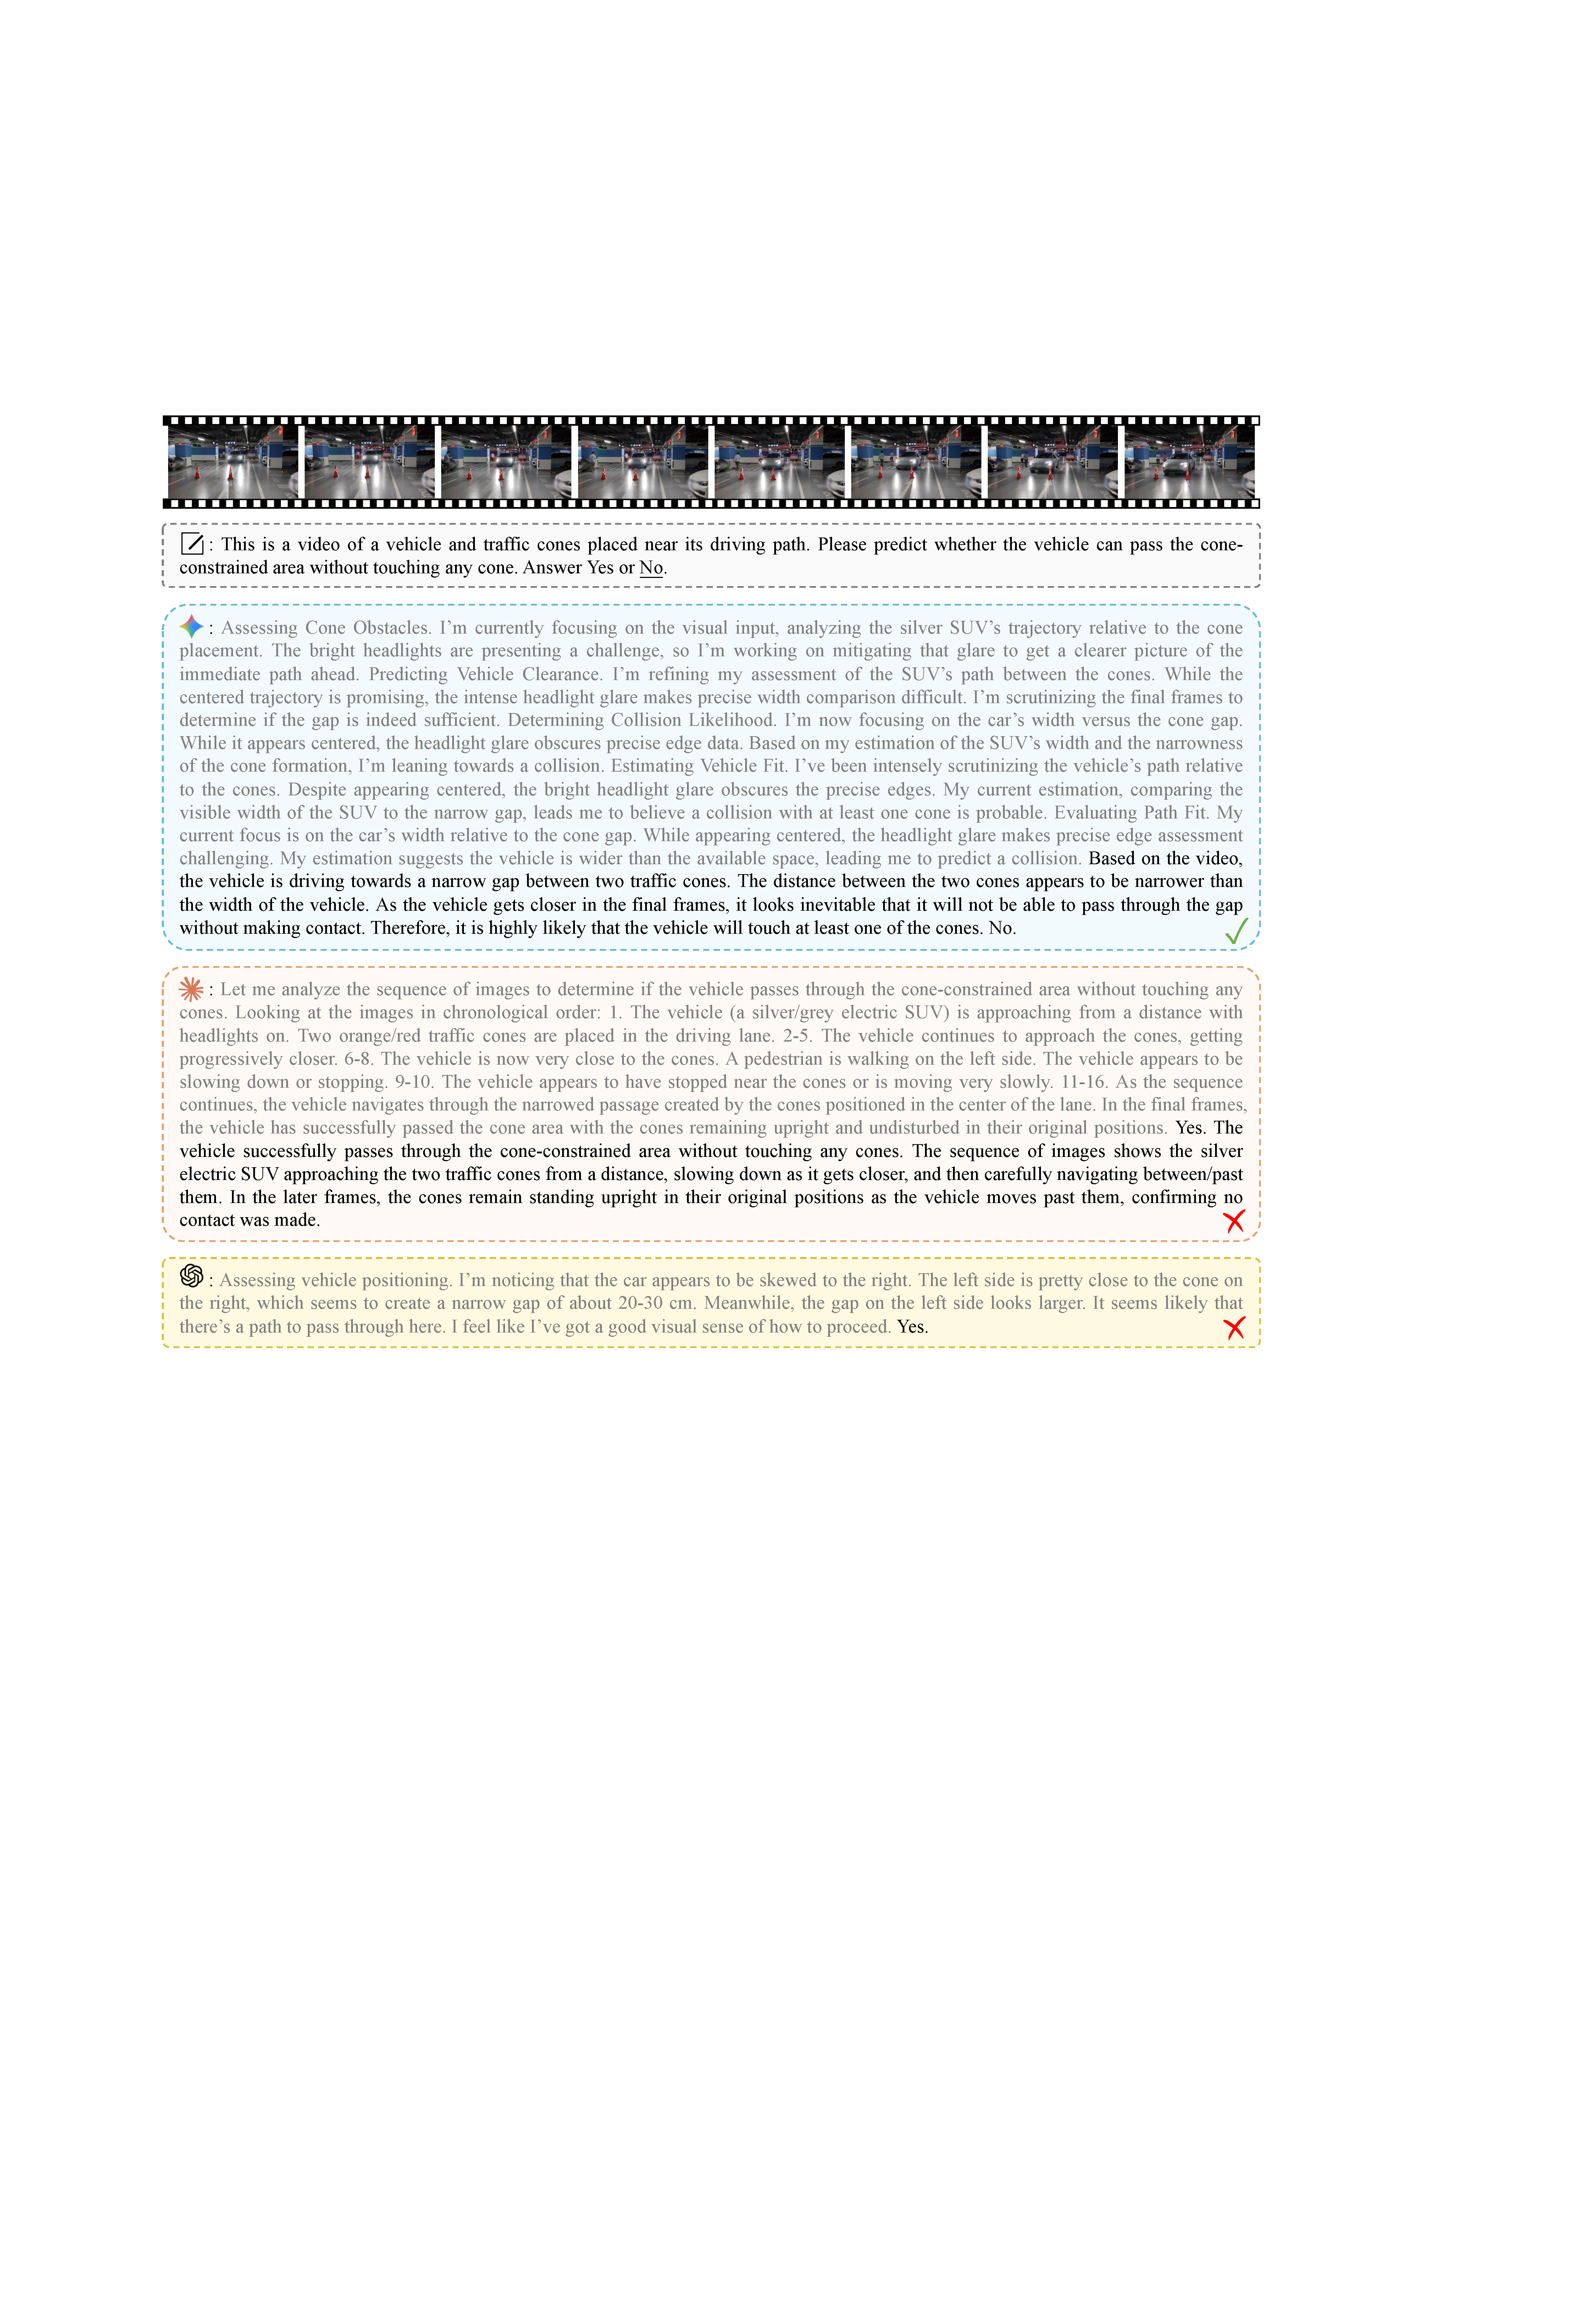
\includegraphics[width=0.95\linewidth]{fig/fig_22.pdf}
  \caption{\textbf{Qualitative visualization for Passage Feasibility.}
  We compare the outputs of GPT-5.4-thinking~\citep{GPT-5}, Gemini-3.1-Pro-Preview~\citep{Gemini}, and Claude-Opus-4.6-thinking~\citep{Claude}.
  Gray text denotes built-in thinking content.}
  \label{fig:22}
\end{figure}

\begin{figure}[p]
  \centering
  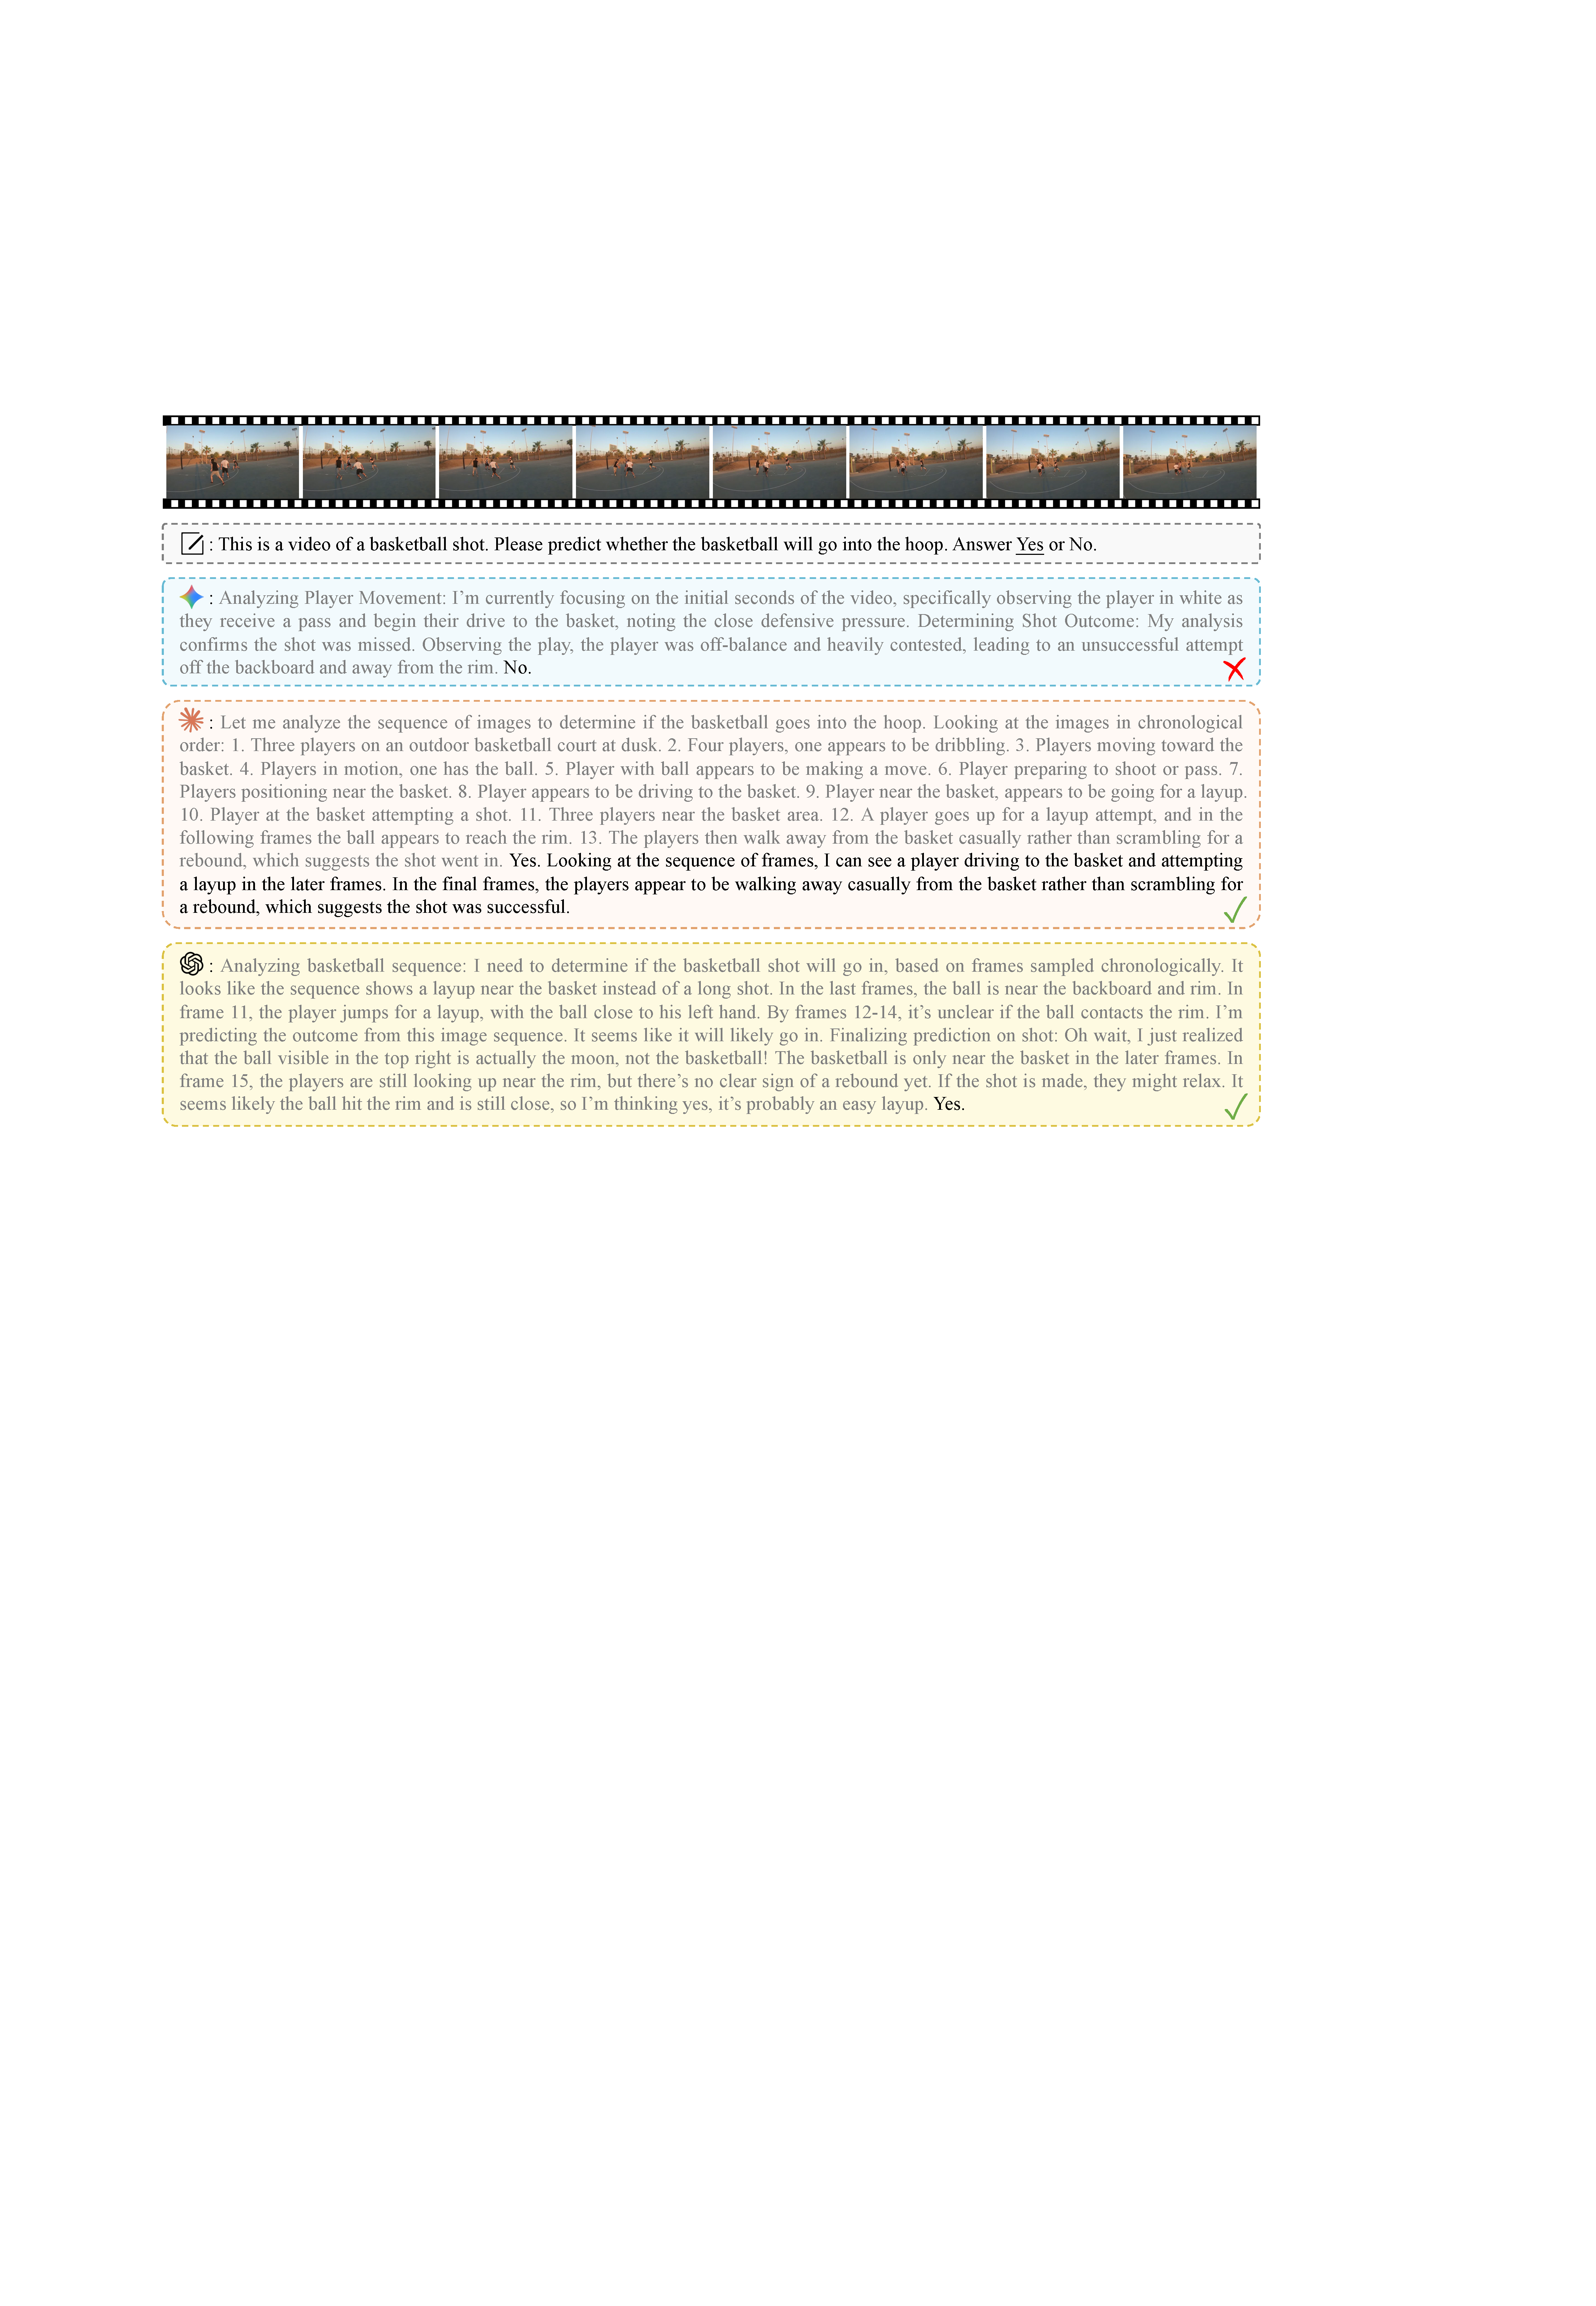
\includegraphics[width=0.95\linewidth]{fig/fig_23.pdf}
  \caption{\textbf{Qualitative visualization for Basketball Shot.}
  We compare the outputs of GPT-5.4-thinking~\citep{GPT-5}, Gemini-3.1-Pro-Preview~\citep{Gemini}, and Claude-Opus-4.6-thinking~\citep{Claude}.
  Gray text denotes built-in thinking content.}
  \label{fig:23}
\end{figure}

\begin{figure}[p]
  \centering
  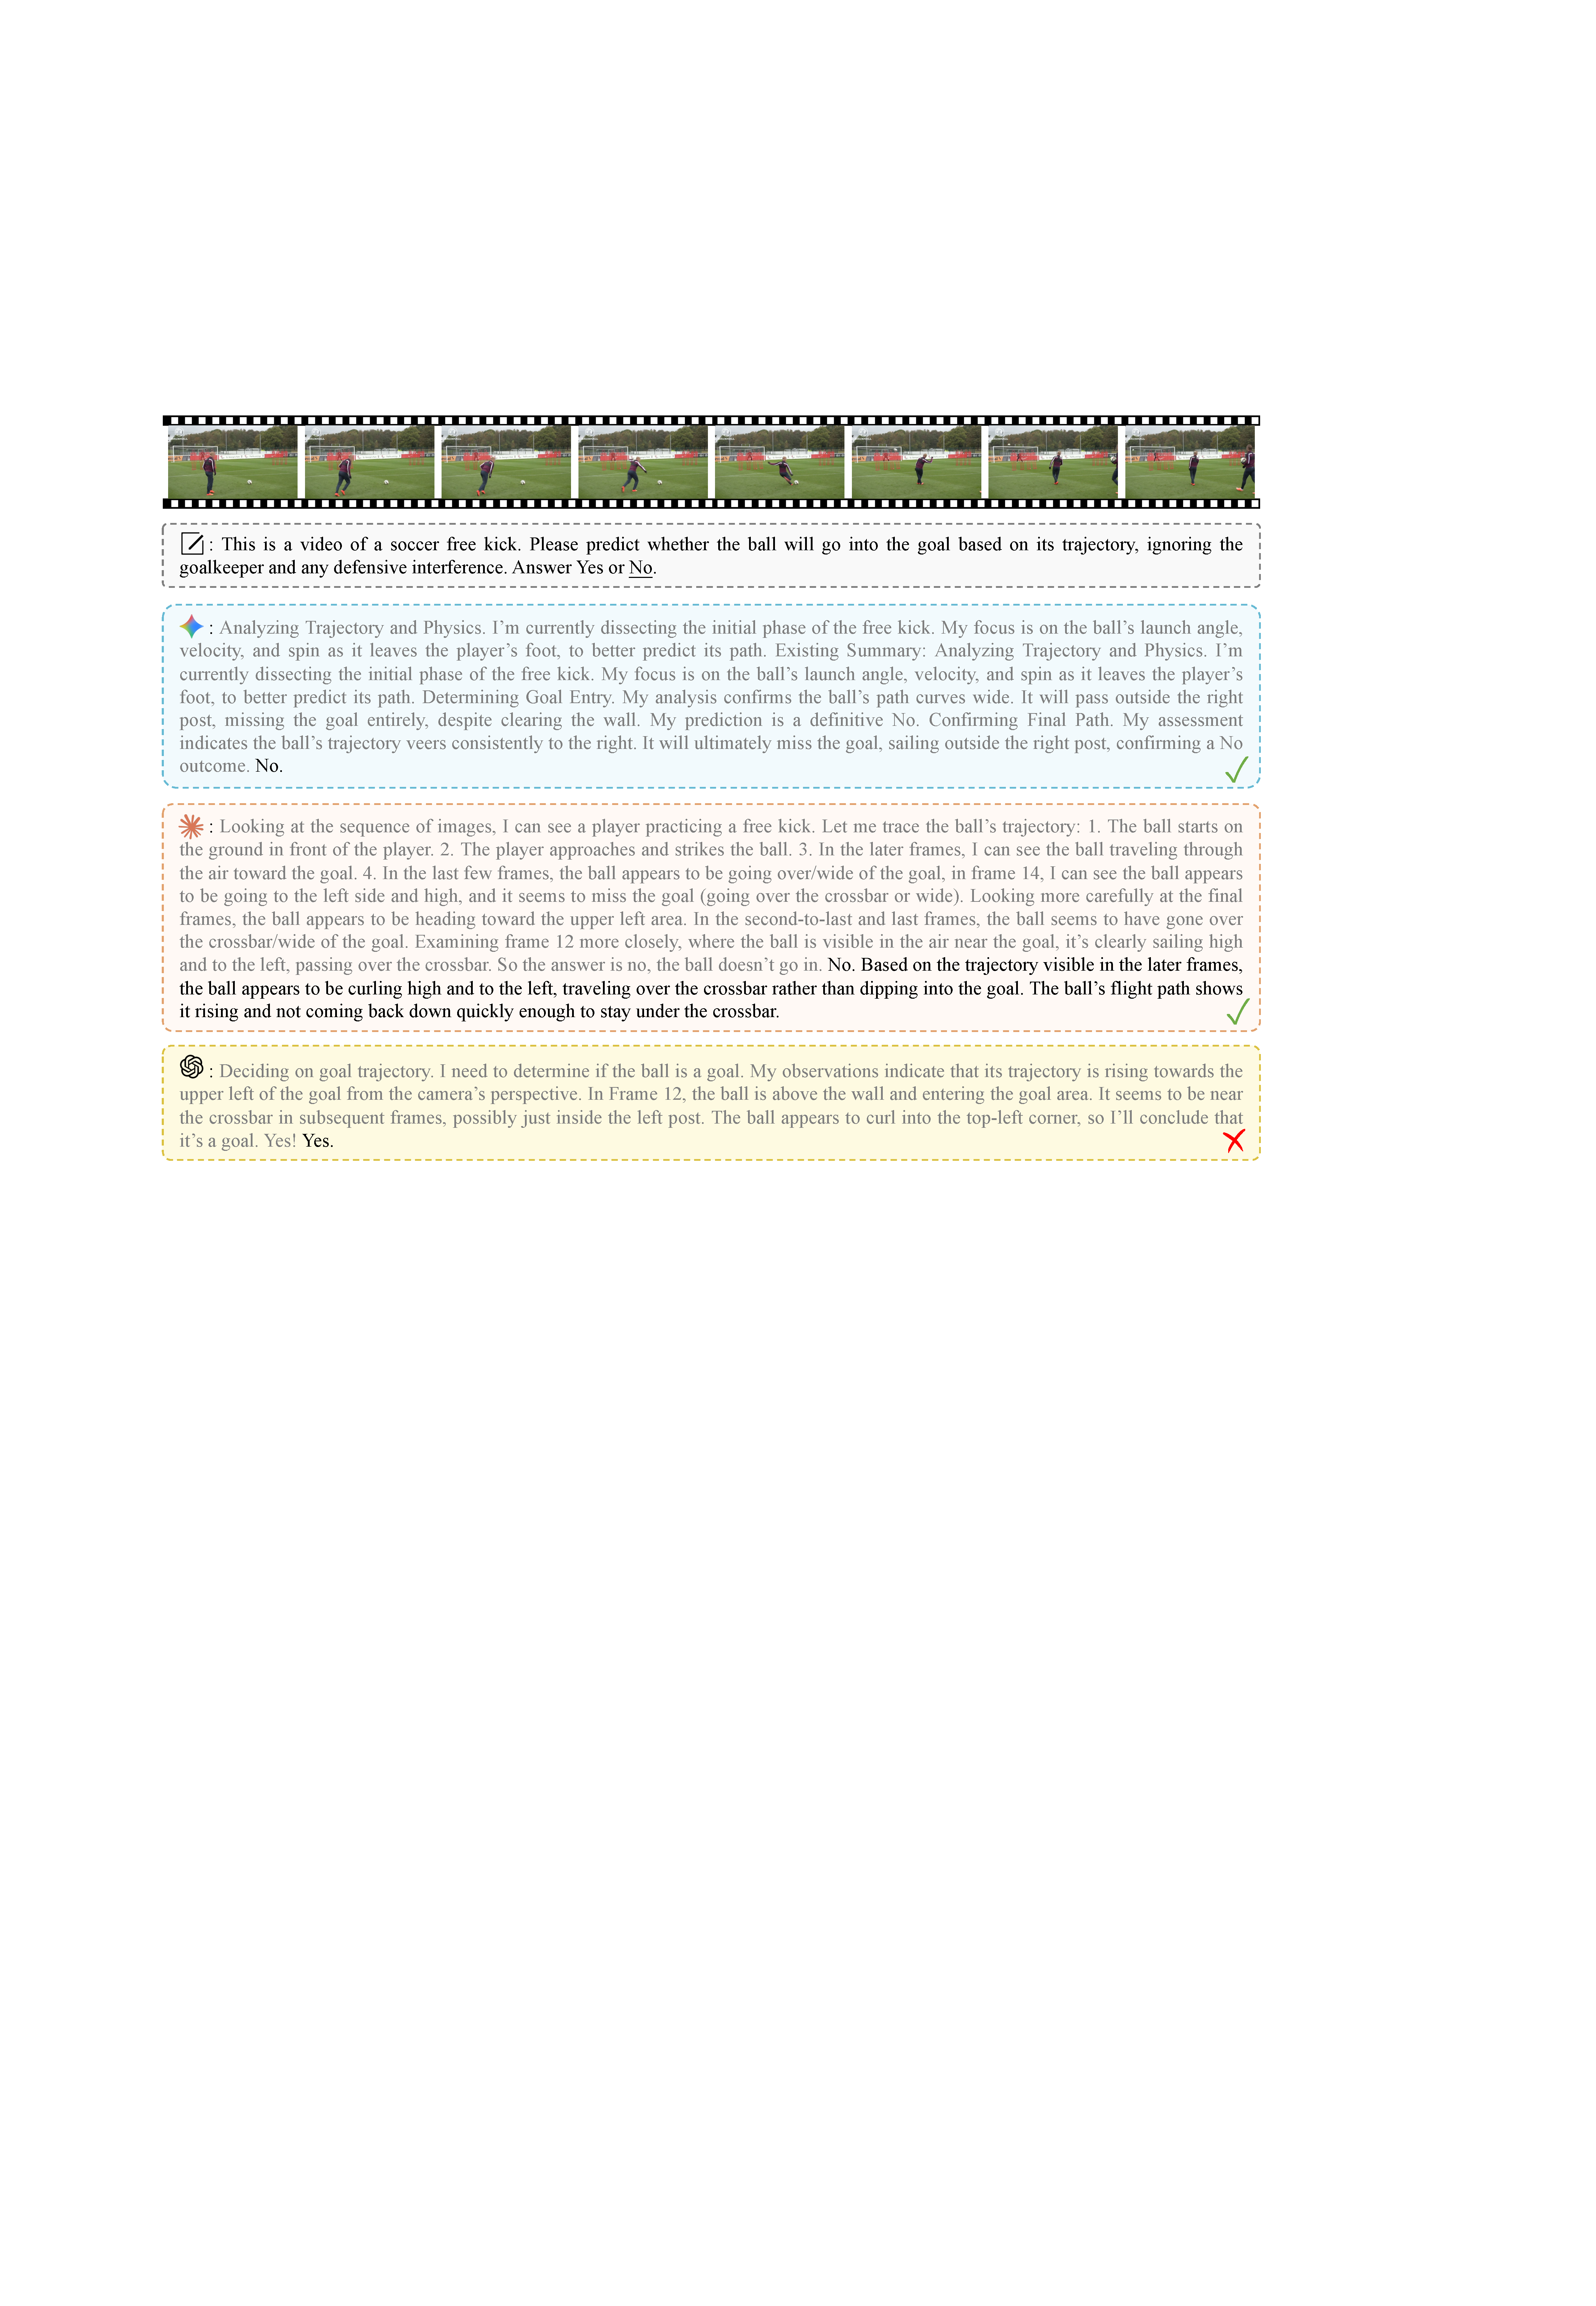
\includegraphics[width=0.95\linewidth]{fig/fig_24.pdf}
  \caption{\textbf{Qualitative visualization for Soccer Shot.}
  We compare the outputs of GPT-5.4-thinking~\citep{GPT-5}, Gemini-3.1-Pro-Preview~\citep{Gemini}, and Claude-Opus-4.6-thinking~\citep{Claude}.
  Gray text denotes built-in thinking content.}
  \label{fig:24}
\end{figure}

\begin{figure}[p]
  \centering
  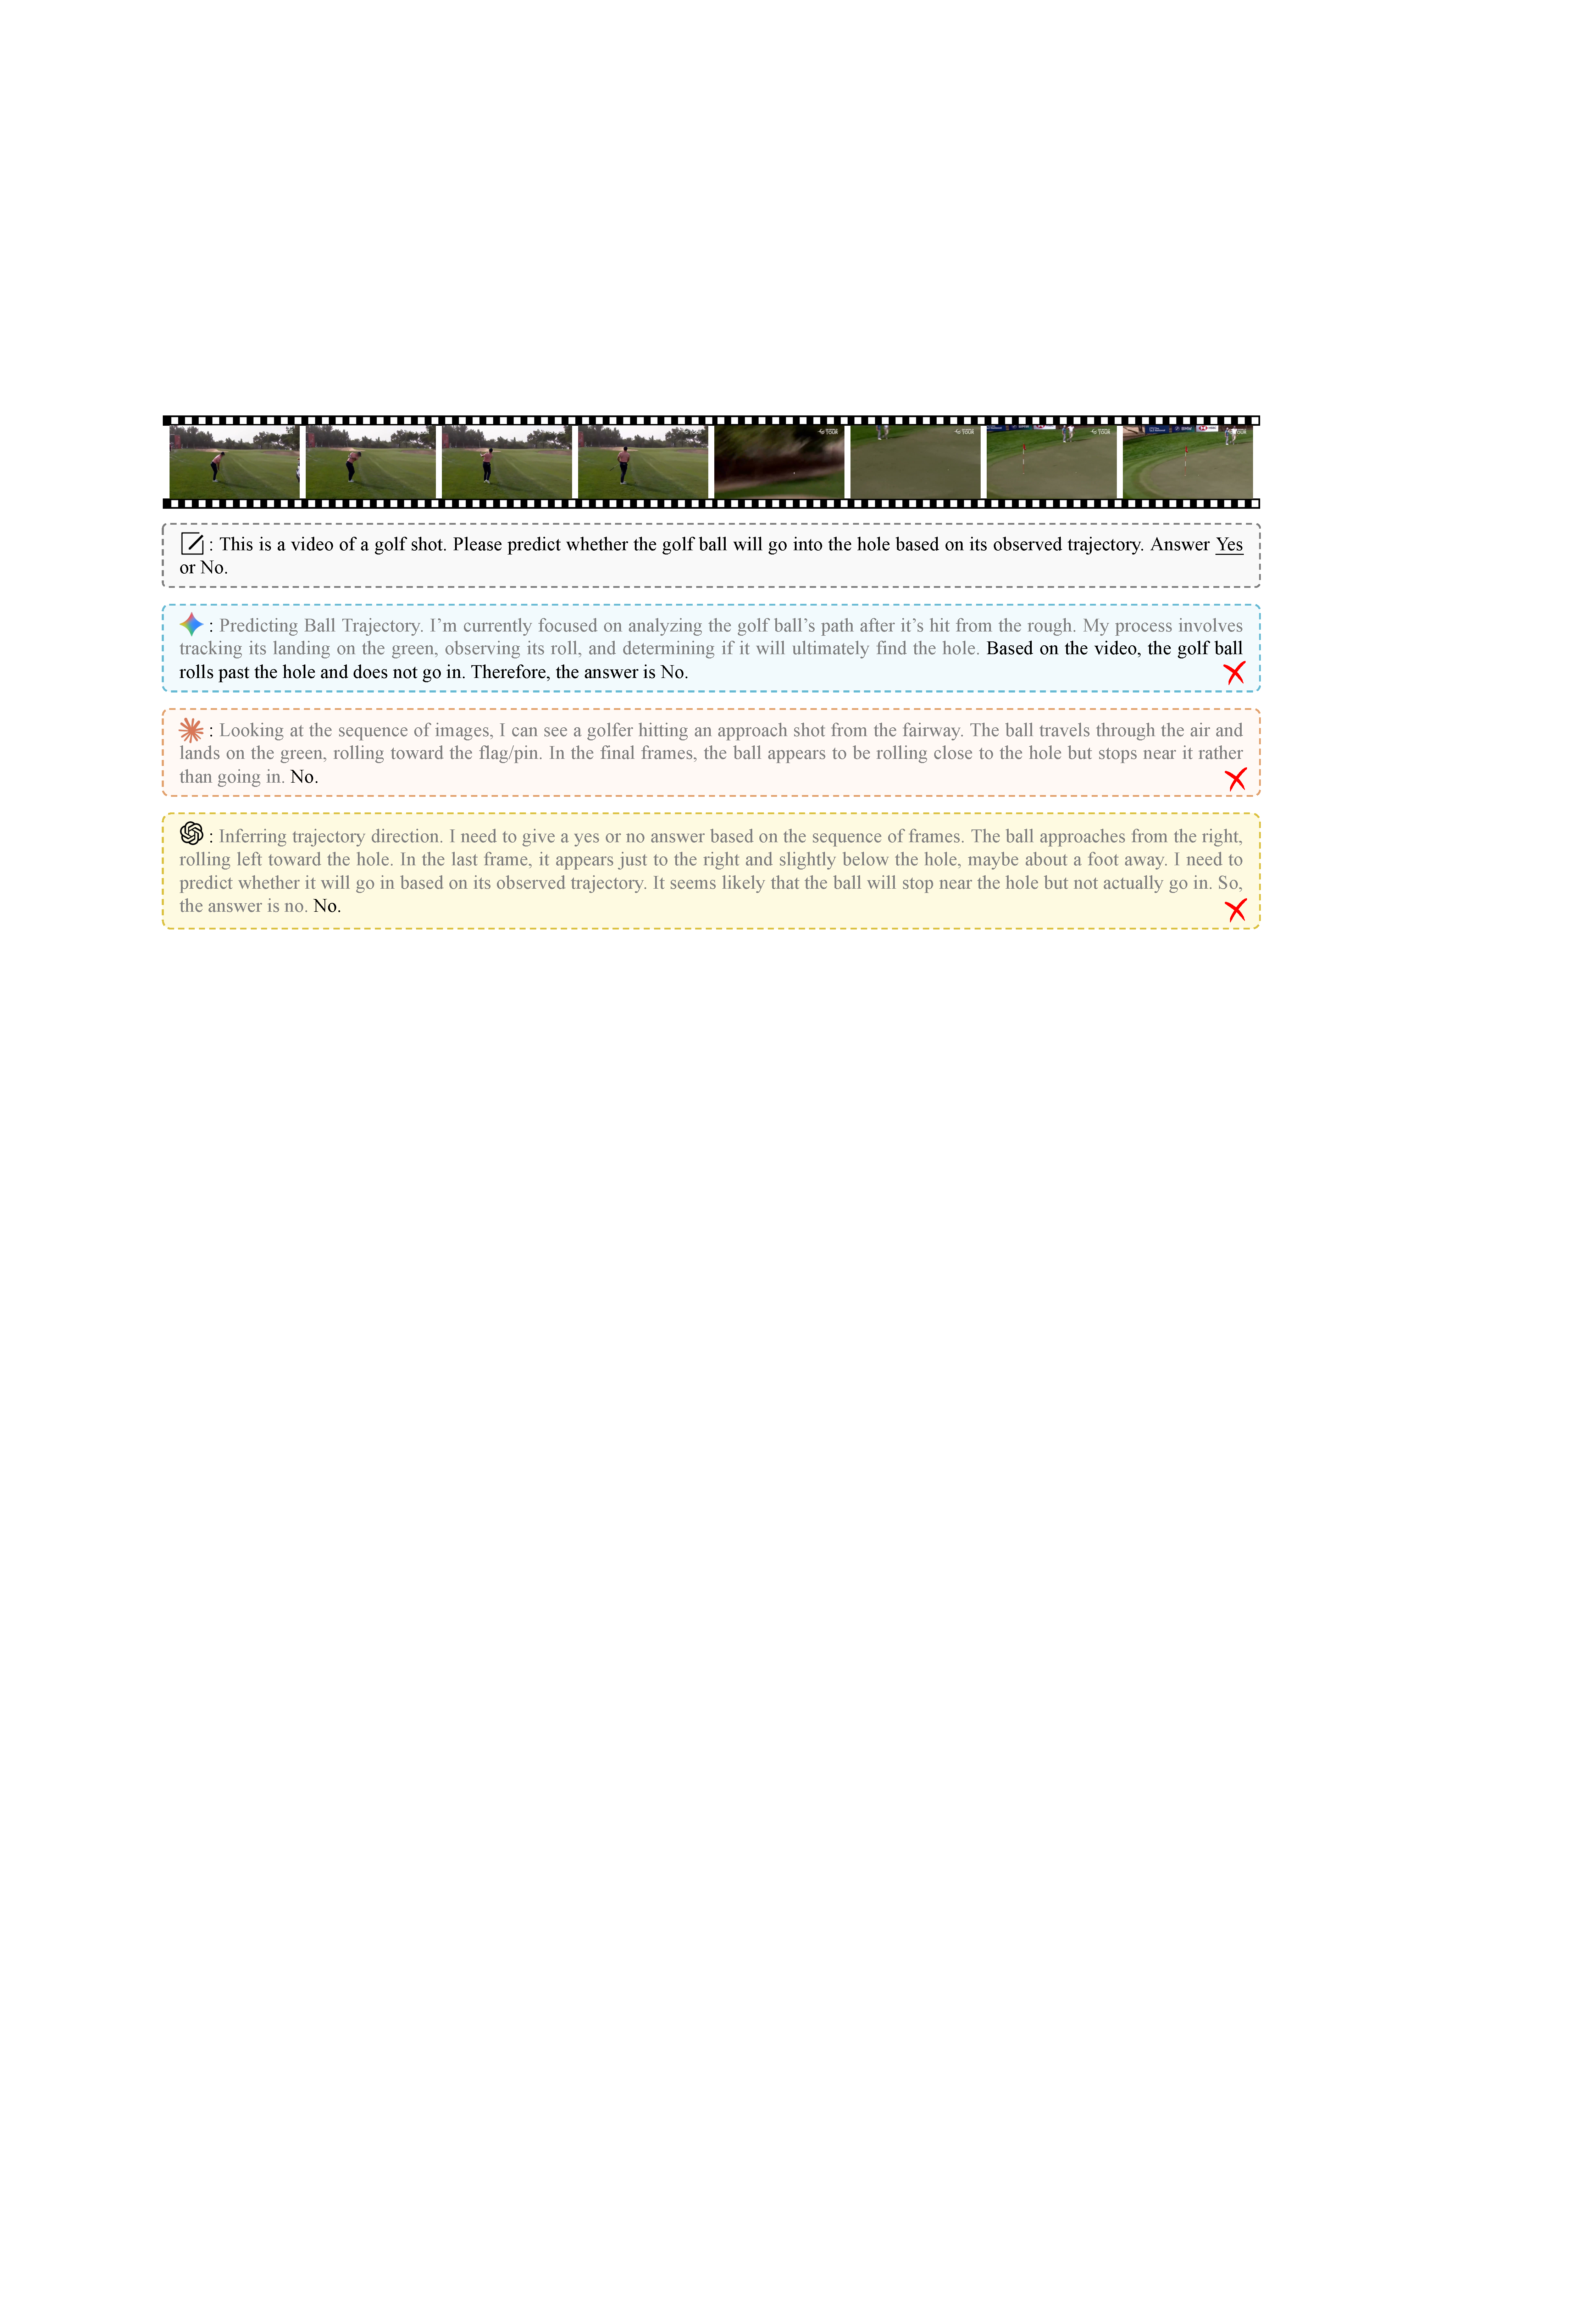
\includegraphics[width=0.95\linewidth]{fig/fig_25.pdf}
  \caption{\textbf{Qualitative visualization for Golf Shot.}
  We compare the outputs of GPT-5.4-thinking~\citep{GPT-5}, Gemini-3.1-Pro-Preview~\citep{Gemini}, and Claude-Opus-4.6-thinking~\citep{Claude}.
  Gray text denotes built-in thinking content.}
  \label{fig:25}
\end{figure}

\begin{figure}[p]
  \centering
  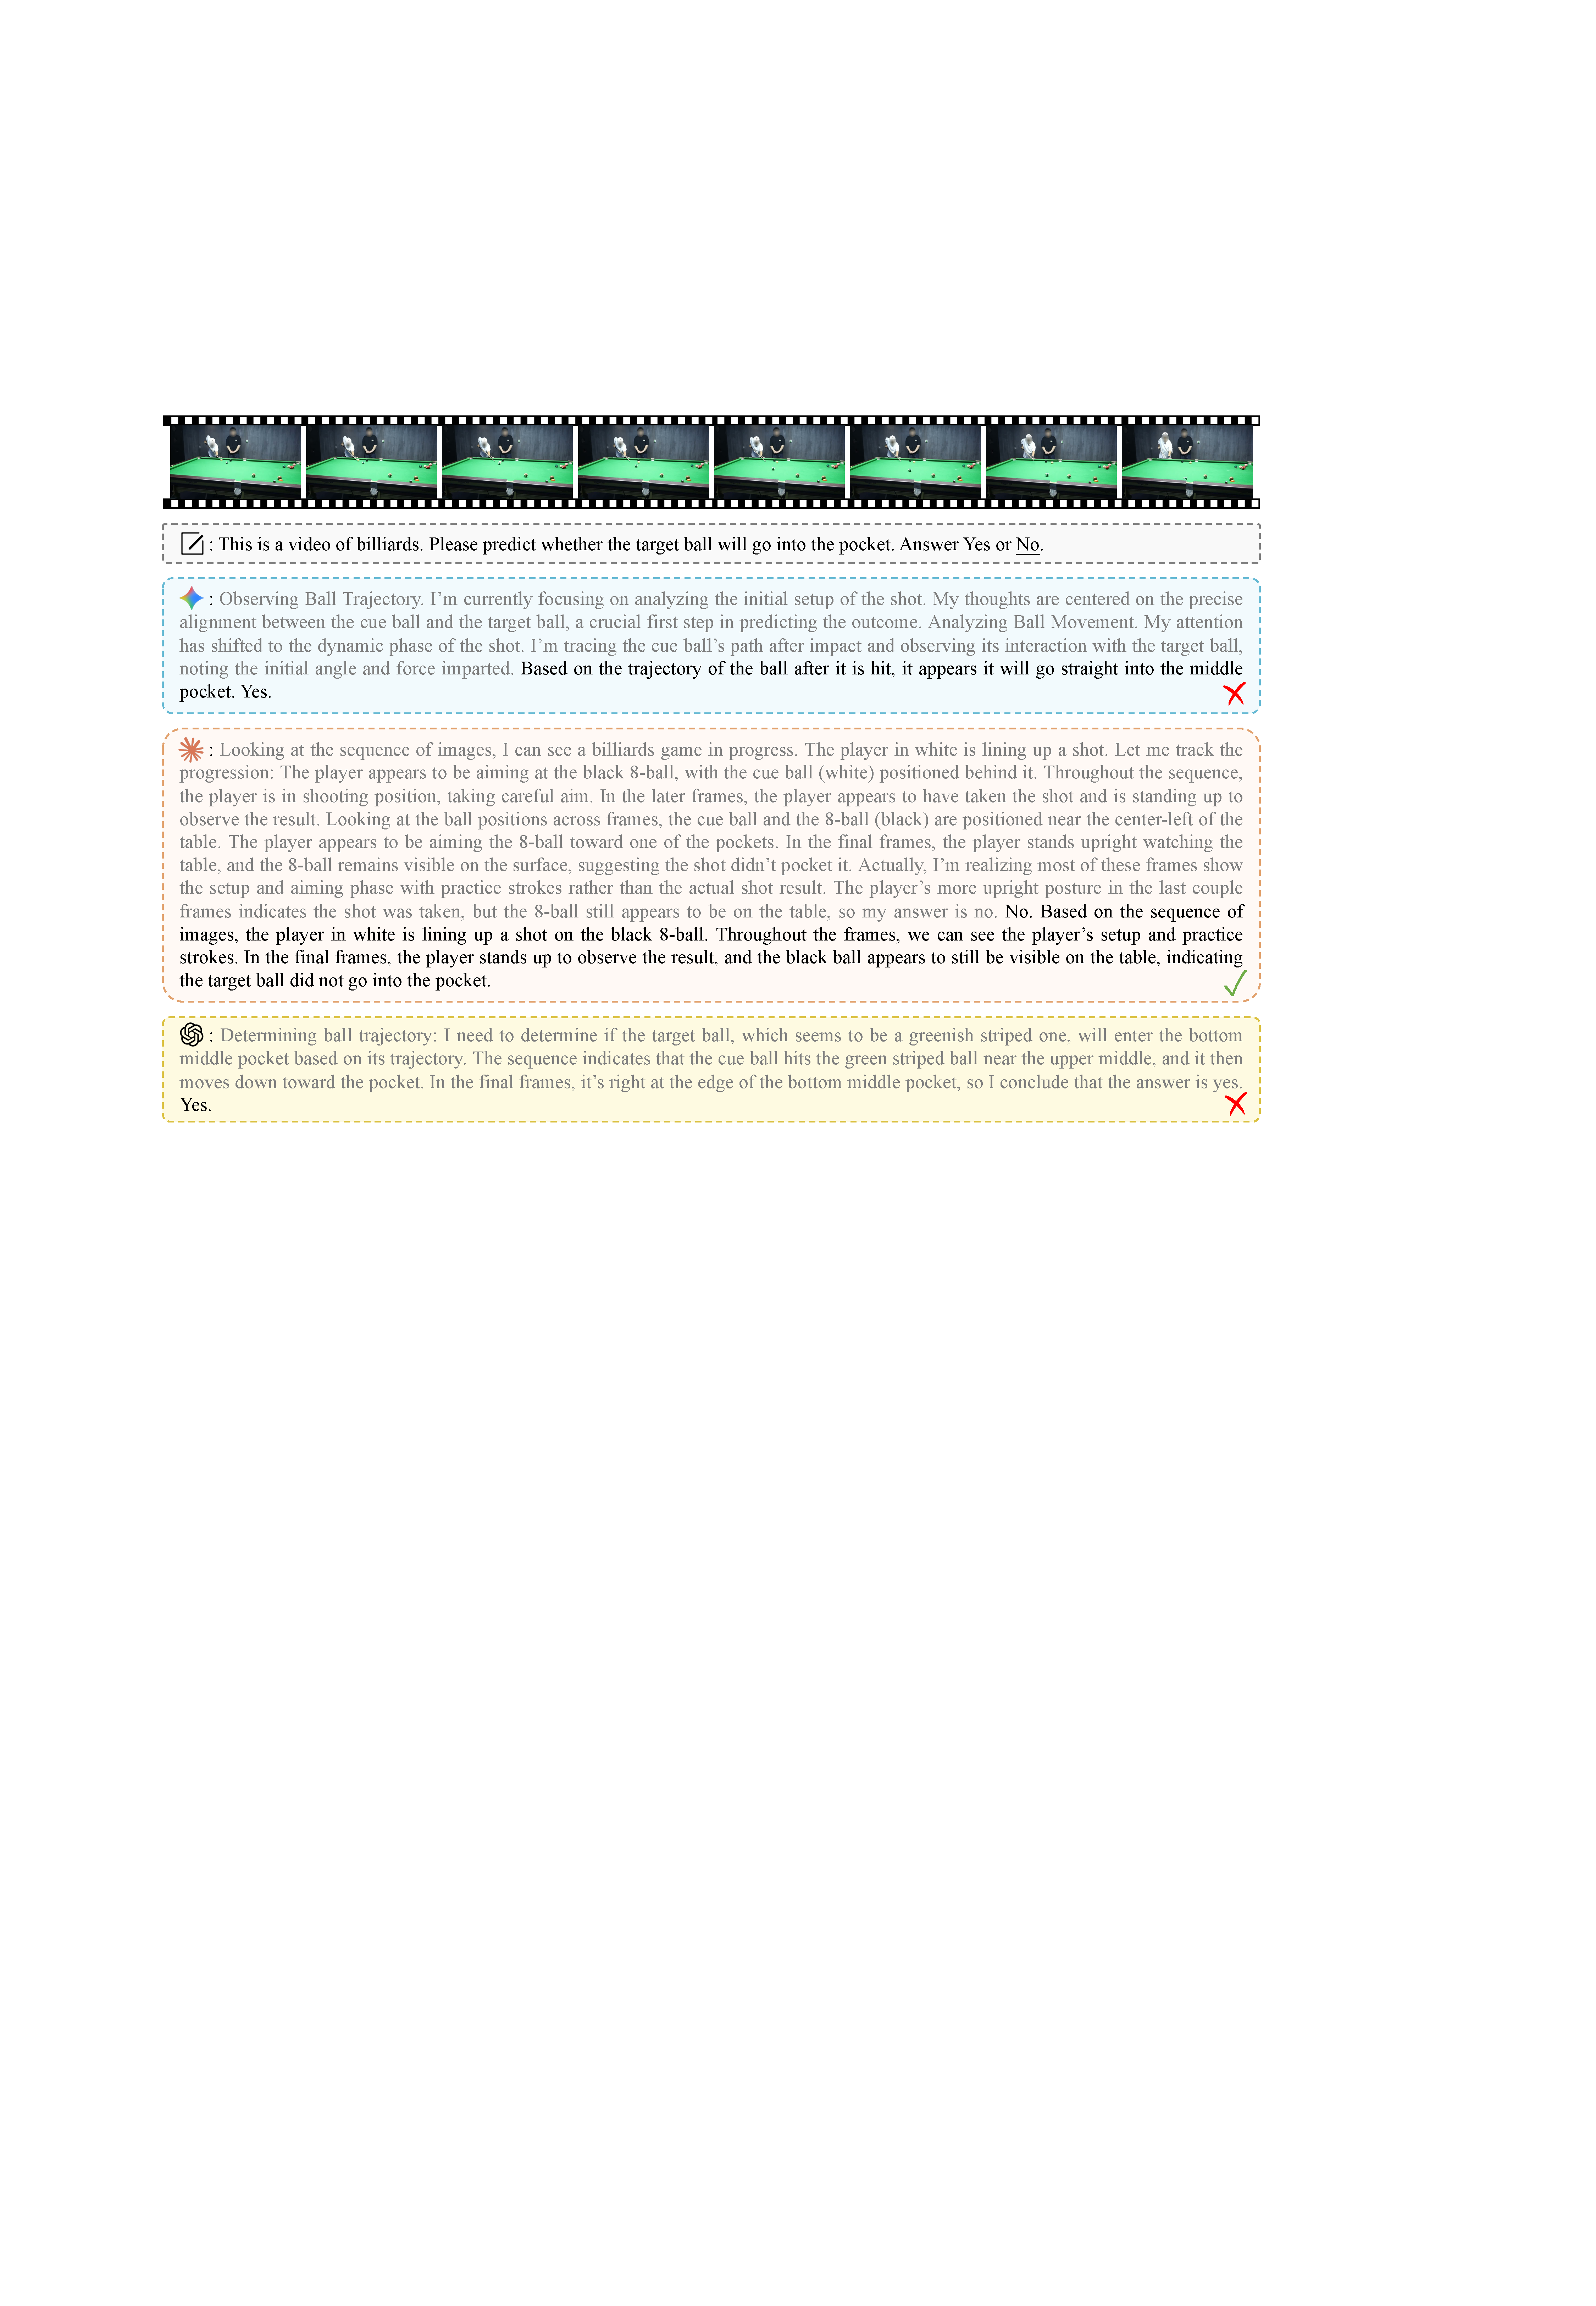
\includegraphics[width=0.95\linewidth]{fig/fig_26.pdf}
  \caption{\textbf{Qualitative visualization for Billiards Shot.}
  We compare the outputs of GPT-5.4-thinking~\citep{GPT-5}, Gemini-3.1-Pro-Preview~\citep{Gemini}, and Claude-Opus-4.6-thinking~\citep{Claude}.
  Gray text denotes built-in thinking content.}
  \label{fig:26}
\end{figure}

\begin{figure}[p]
  \centering
  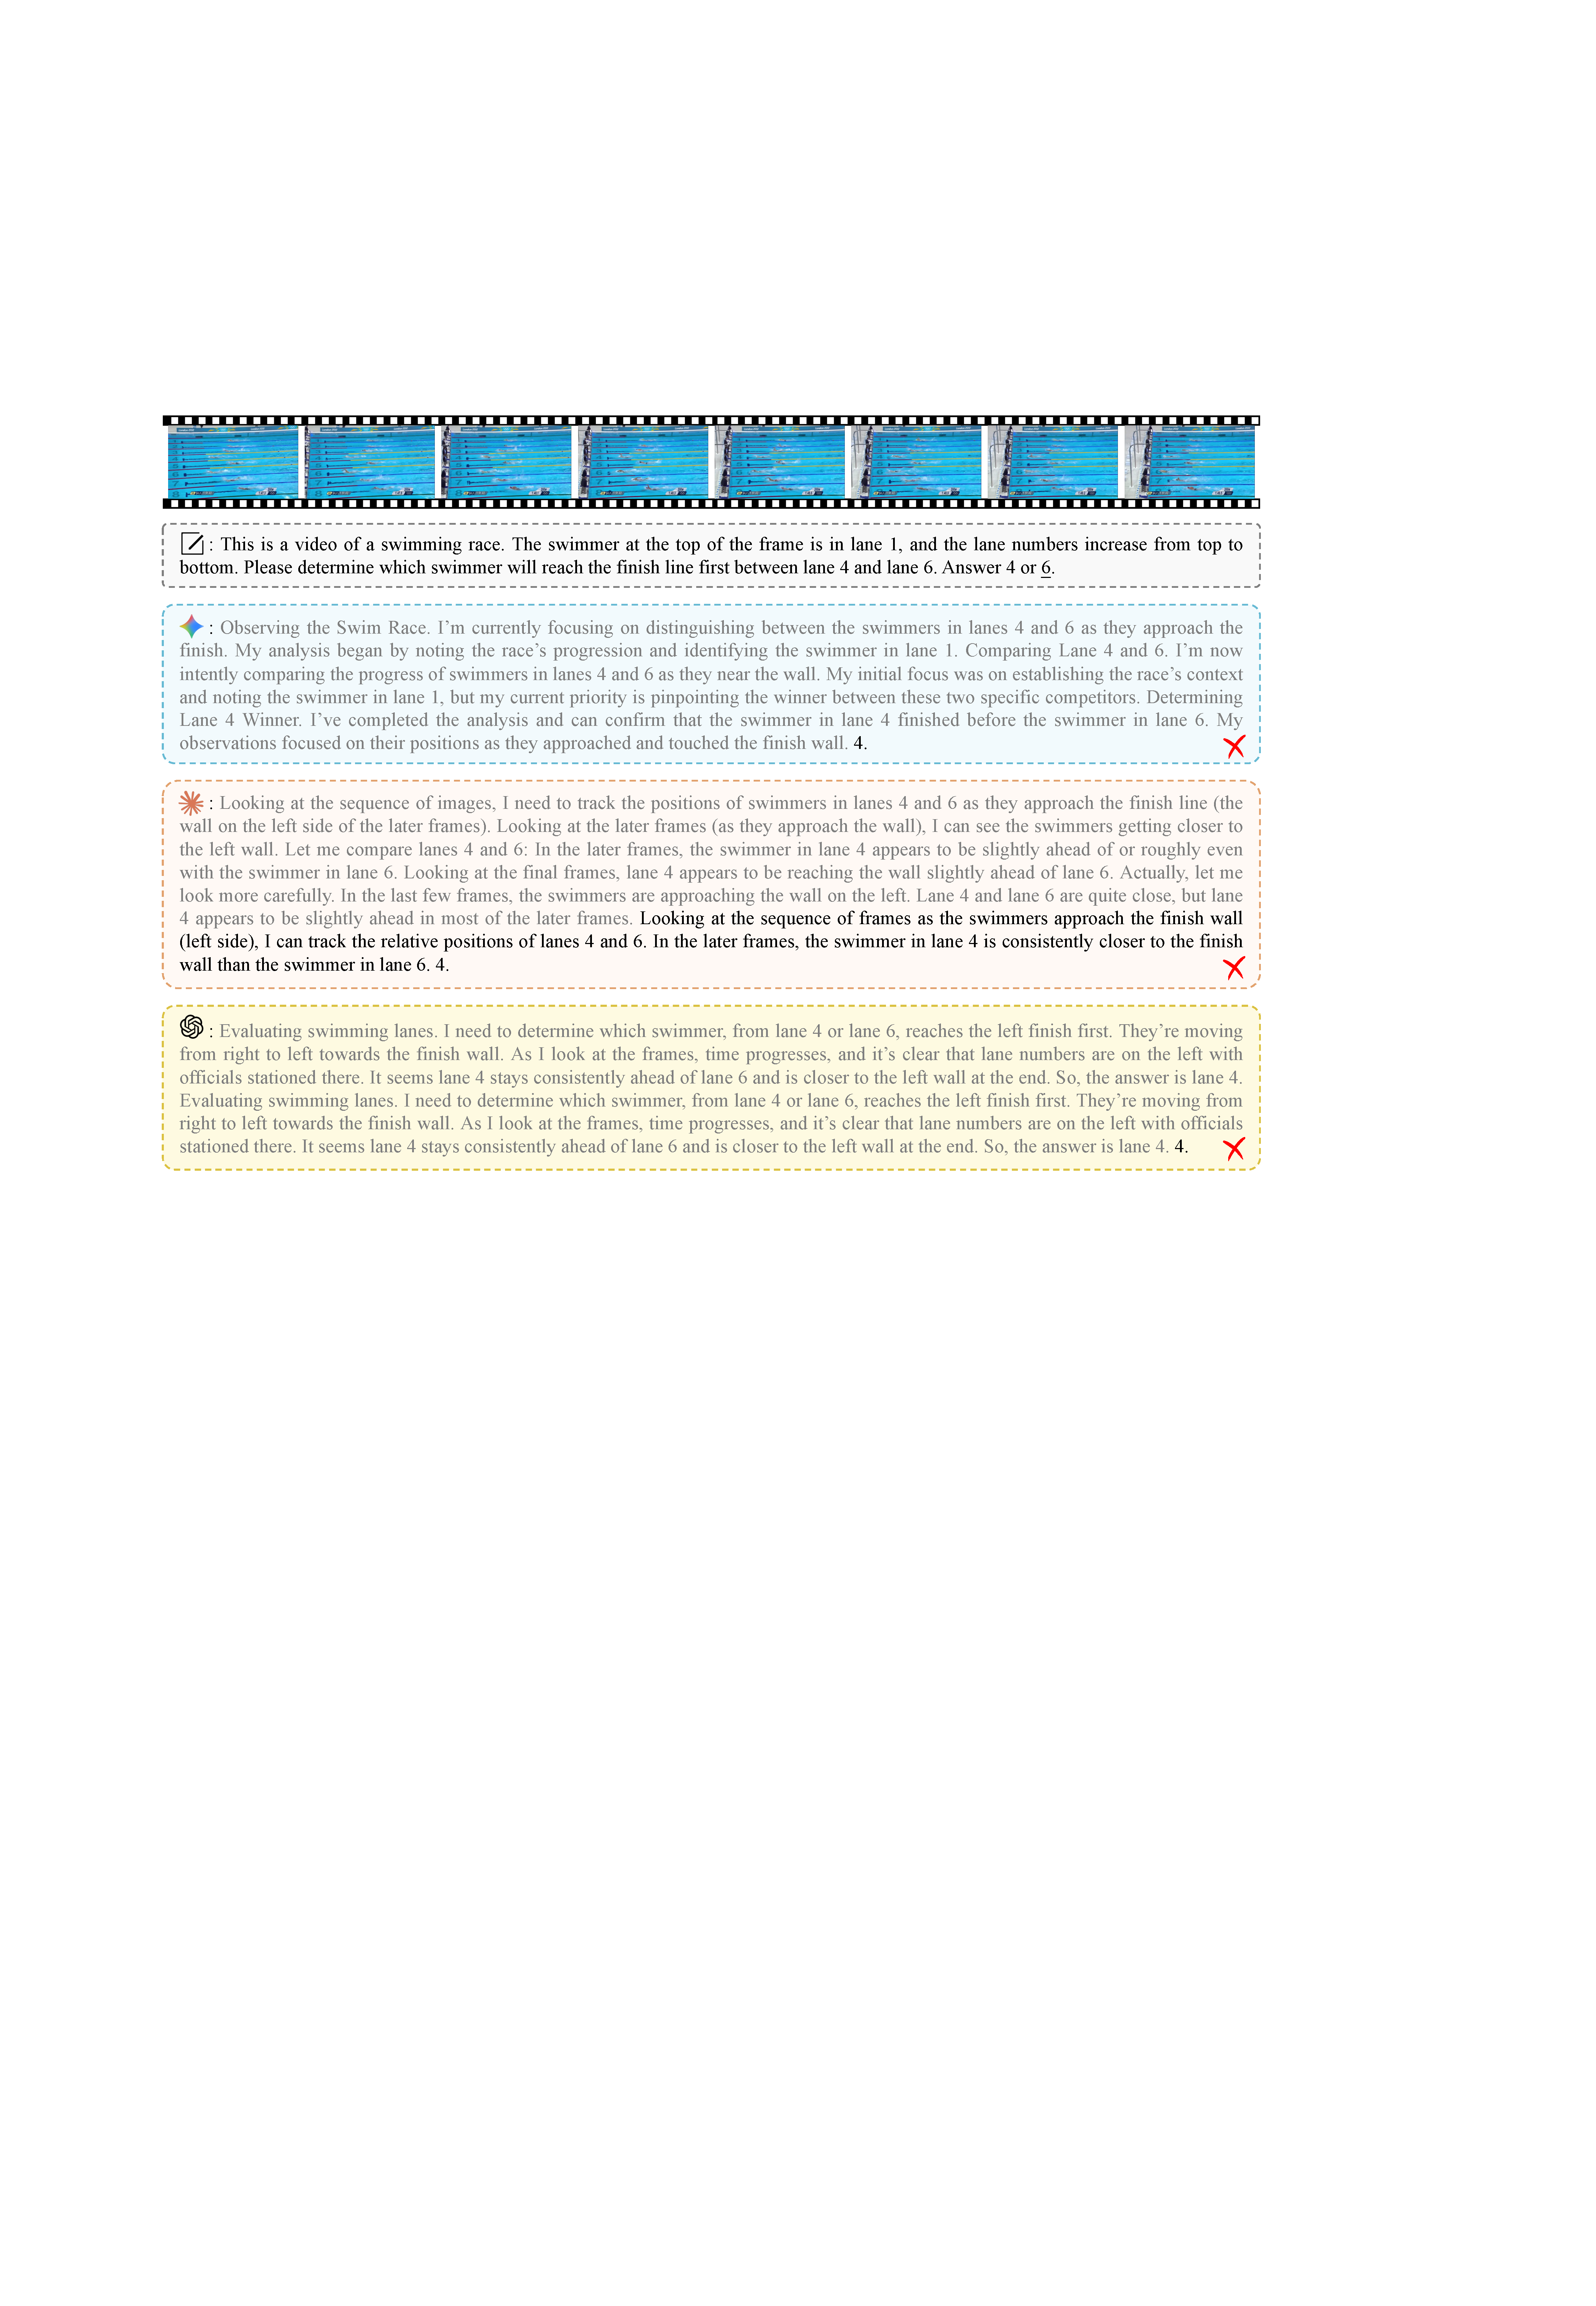
\includegraphics[width=0.95\linewidth]{fig/fig_27.pdf}
  \caption{\textbf{Qualitative visualization for Swimming Race.}
  We compare the outputs of GPT-5.4-thinking~\citep{GPT-5}, Gemini-3.1-Pro-Preview~\citep{Gemini}, and Claude-Opus-4.6-thinking~\citep{Claude}.
  Gray text denotes built-in thinking content.}
  \label{fig:27}
\end{figure}

\begin{figure}[p]
  \centering
  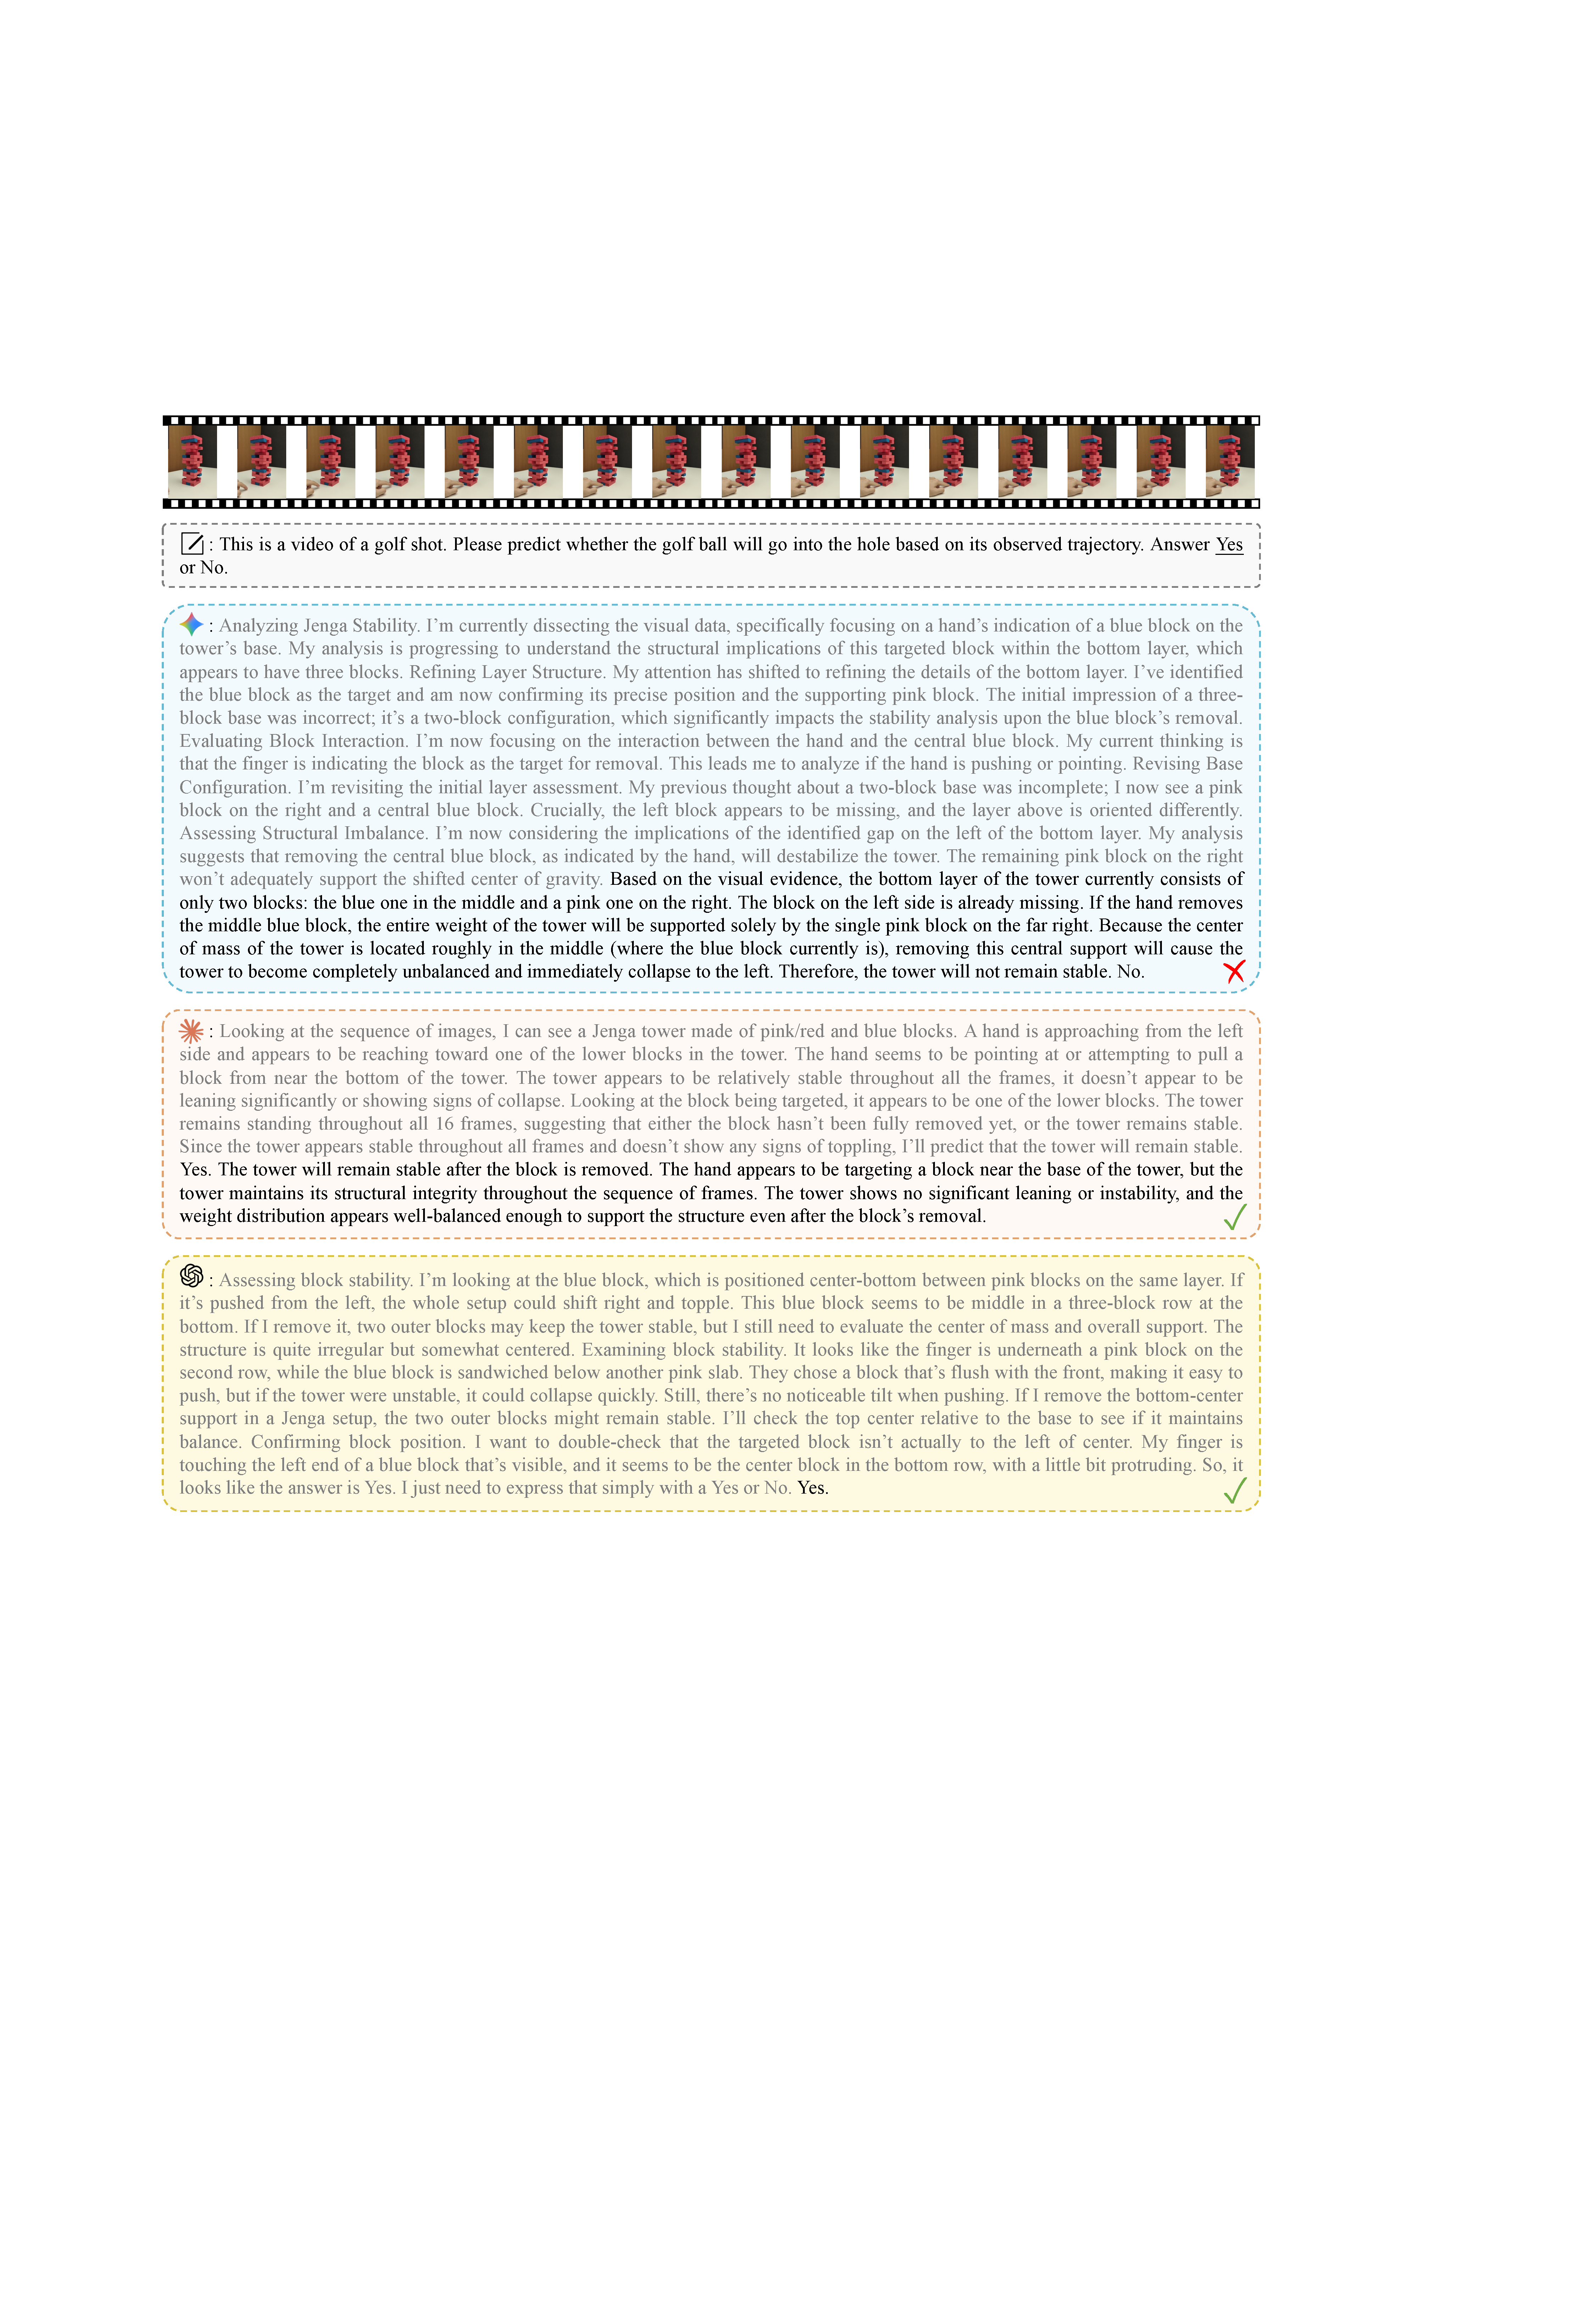
\includegraphics[width=0.95\linewidth]{fig/fig_28.pdf}
  \caption{\textbf{Qualitative visualization for Jenga Stability.}
  We compare the outputs of GPT-5.4-thinking~\citep{GPT-5}, Gemini-3.1-Pro-Preview~\citep{Gemini}, and Claude-Opus-4.6-thinking~\citep{Claude}.
  Gray text denotes built-in thinking content.}
  \label{fig:28}
\end{figure}

\begin{figure}[p]
  \centering
  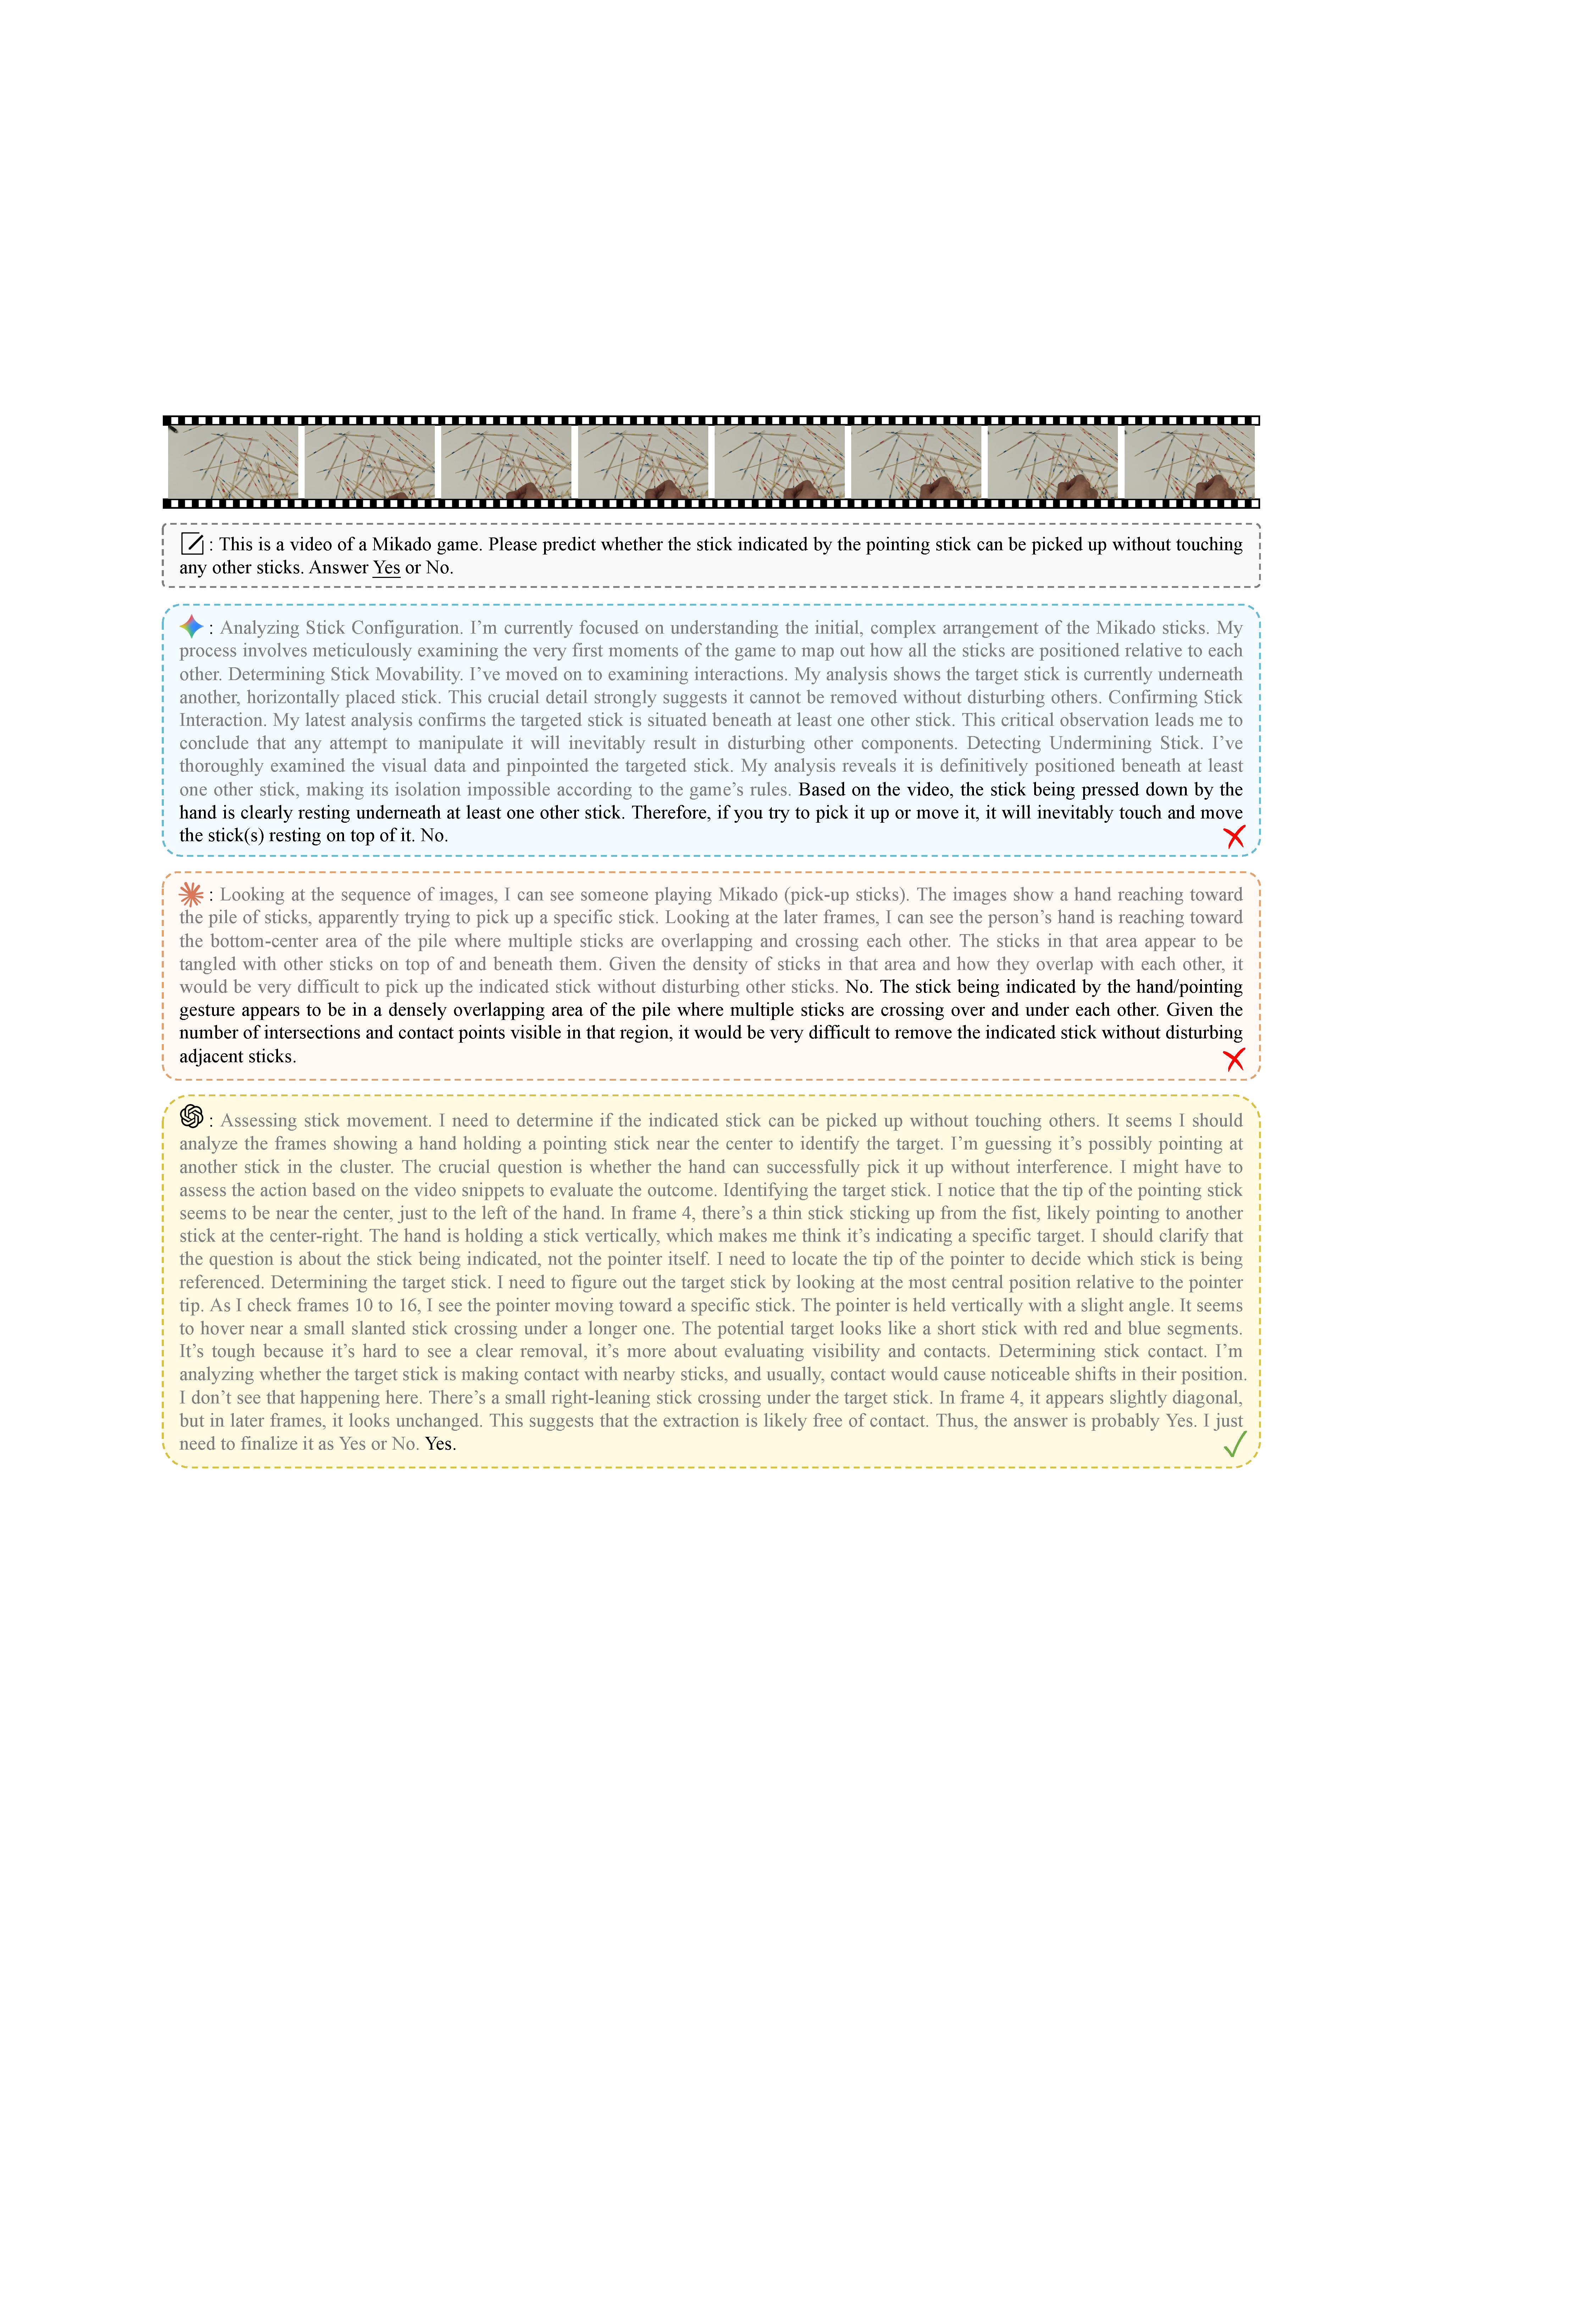
\includegraphics[width=0.95\linewidth]{fig/fig_29.pdf}
  \caption{\textbf{Qualitative visualization for Mikado Dependency.}
  We compare the outputs of GPT-5.4-thinking~\citep{GPT-5}, Gemini-3.1-Pro-Preview~\citep{Gemini}, and Claude-Opus-4.6-thinking~\citep{Claude}.
  Gray text denotes built-in thinking content.}
  \label{fig:29}
\end{figure}

\begin{figure}[p]
  \centering
  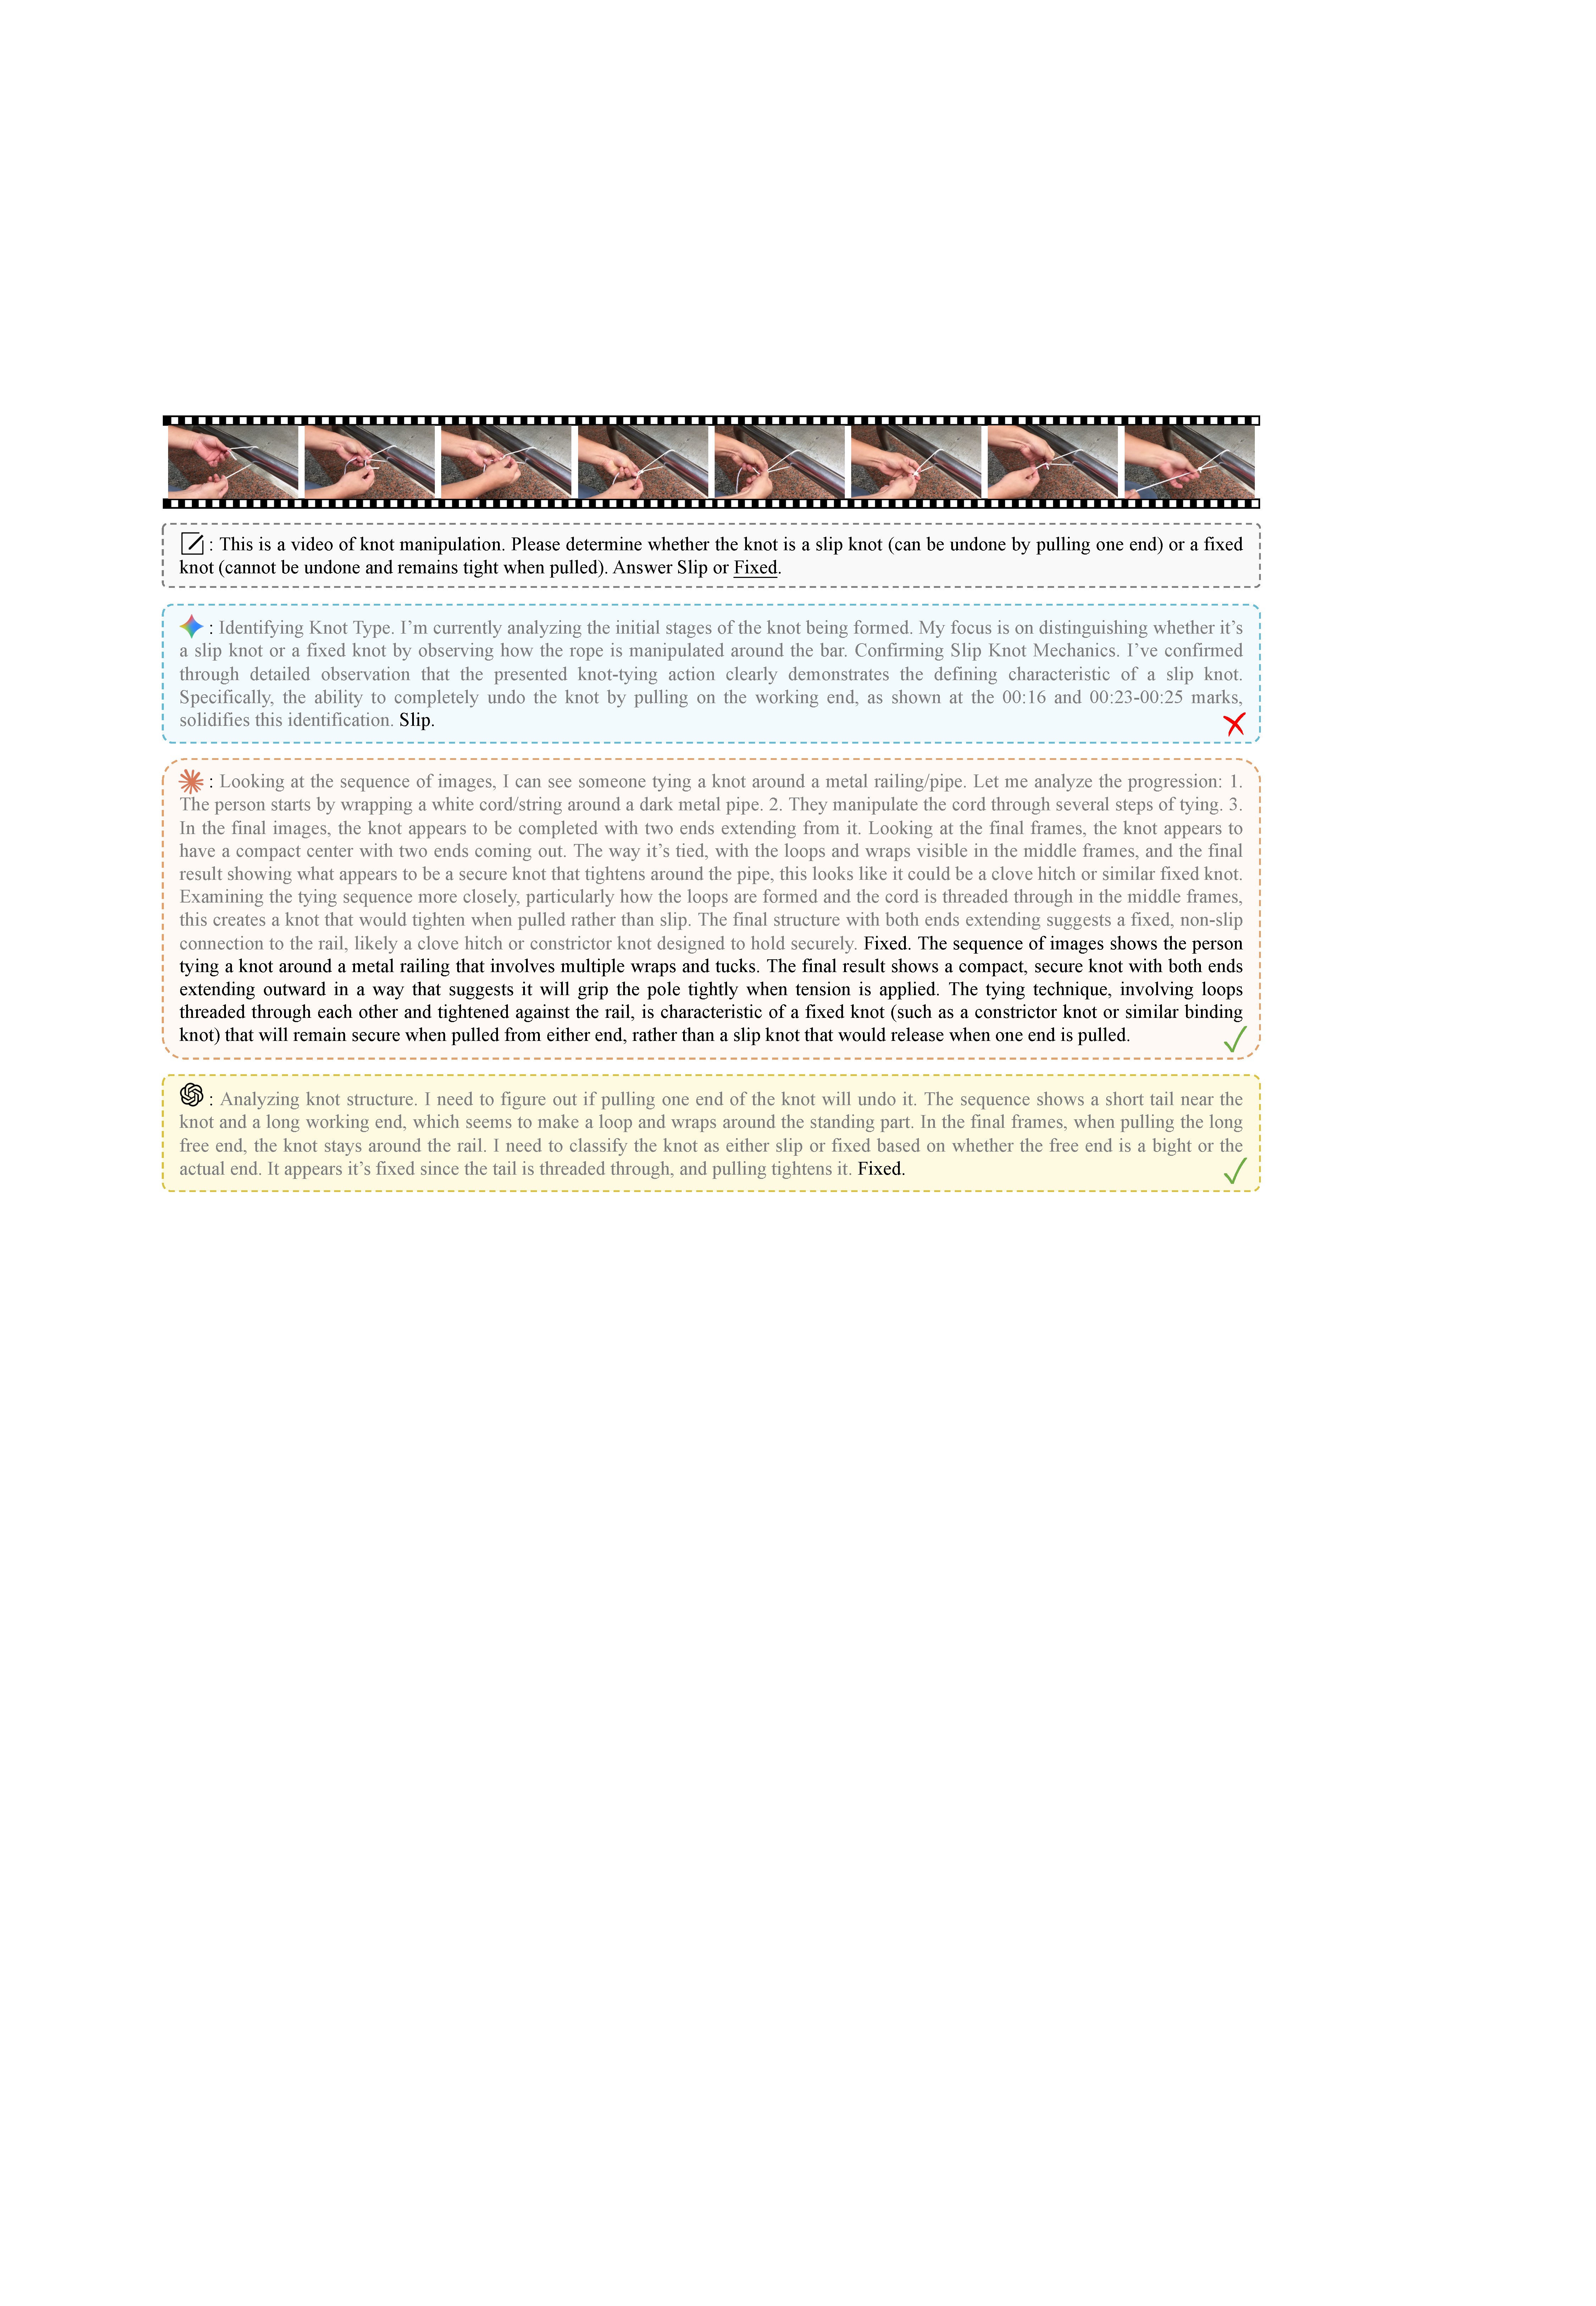
\includegraphics[width=0.95\linewidth]{fig/fig_30.pdf}
  \caption{\textbf{Qualitative visualization for Knot Type.}
  We compare the outputs of GPT-5.4-thinking~\citep{GPT-5}, Gemini-3.1-Pro-Preview~\citep{Gemini}, and Claude-Opus-4.6-thinking~\citep{Claude}.
  Gray text denotes built-in thinking content.}
  \label{fig:30}
\end{figure}
